% !TeX encoding = UTF-8

% 载入 SJTUThesis 模版
\documentclass[type=master]{sjtuthesis}
% 选项
%   type=[doctor|master|bachelor],     % 可选(默认:master),论文类型
%   zihao=[-4|5],                      % 可选(默认:-4),正文字号大小
%   lang=[zh|en|de|ja],                % 可选(默认:zh),论文的主要语言
%   review,                            % 可选(默认:关闭),盲审模式
%   [twoside|oneside],                 % 可选(默认:twoside),双页或单页边距模式
%   [openright|openany],               % 可选(默认:openright),奇数页或任意页开始新章
%   math-style=[ISO|TeX],              % 可选 (默认:ISO),数学符号样式

% 论文基本配置,加载宏包等全局配置
% !TEX root = ./main.tex

\sjtusetup{
  %
  %******************************
  % 注意:
  %   1. 配置里面不要出现空行
  %   2. 不需要的配置信息可以删除
  %******************************
  %
  % 信息录入
  %
  info = {%
    %
    % 标题
    %
    zh / title           = {基于高阶全驱系统理论的四旋翼飞行器最优控制},
    en / title           = {A Sample Document for \LaTeX-based SJTU Thesis Template},
    %
    % 标题页标题
    %   可使用“\\”命令手动控制换行
    %
    % zh / display-title   = {上海交通大学学位论文\\ \LaTeX{} 模板示例文档},
    % en / display-title   = {A Sample Document \\ for \LaTeX-based SJTU Thesis Template},
    %
    % 关键词
    %
    zh / keywords        = {上海交大, 饮水思源, 爱国荣校},
    en / keywords        = {SJTU, master thesis, XeTeX/LaTeX template},
    %
    % 姓名
    %
    zh / author          = {赵泽源},
    en / author          = {Zeyuan Zhao},
    %
    % 指导教师
    %
    zh / supervisor      = {李贤伟教授},
    en / supervisor      = {Prof. Xianwei Li},
    %
    % 副指导教师
    %
    % assoc-supervisor  = {某某教授},
    % assoc-supervisor* = {Prof. Uom Uom},
    %
    % 学号
    %
    id              = {520021910884},
    %
    % 学位
    %   本科生不需要填写
    %
    zh / degree          = {工学硕士},
    en / degree          = {Master of Engineering},
    %
    % 专业
    %
    zh / major           = {自动化},
    en / major           = {Automatic},
    %
    % 所属院系
    %
    zh / department      = {电子信息与电气工程学院},
    en / department      = {School of Electronic Information and Electrical Engineering},
    %
    % 答辩日期
    %   使用 ISO 格式 (yyyy-mm-dd);默认为当前时间
    %
    % date                 = {2023-05-18},
    %
    % 标题页显示日期
    %   覆盖对应标题页的日期显示,原样输出
    %
    % zh / display-date    = {2023 年 5 月},
    %
    % 资助基金
    %
    % zh / fund  = {
    %                {国家 973 项目 (No. 2025CB000000)},
    %                {国家自然科学基金 (No. 81120250000)},
    %              },
    % en / fund  = {
    %                {National Basic Research Program of China (Grant No. 2025CB000000)},
    %                {National Natural Science Foundation of China (Grant No. 81120250000)},
    %              },
  },
  %
  % 风格设置
  %
  style = {%
    %
    % 论文标题页 logo 颜色 (red/blue/black)
    %
    % title-logo-color = black,
  },
  %
  % 名称设置
  %
  name = {
    % bib             = {References},
    % ack             = {谢\hspace{\ccwd}辞},
    % achv            = {攻读学位期间完成的论文},
  },
}

% 使用 BibLaTeX 处理参考文献
%   biblatex-gb7714-2015 常用选项
%     gbnamefmt=lowercase     姓名大小写由输入信息确定
%     gbpub=false             禁用出版信息缺失处理
\usepackage[backend=biber,style=gb7714-2015]{biblatex}
% 文献表字体
% \renewcommand{\bibfont}{\zihao{5}\fixedlineskip{15.6bp}}
% 文献表条目间的间距
\setlength{\bibitemsep}{0pt}
% 导入参考文献数据库
\addbibresource{refs.bib}

% 脚注格式
\usepackage[perpage,bottom,hang]{footmisc}

% 定义图片文件目录与扩展名
\graphicspath{{figures/}{matlab_figures/}}

\DeclareGraphicsExtensions{.pdf,.eps,.png,.jpg,.jpeg}

% 确定浮动对象的位置,可以使用 [H],强制将浮动对象放到这里(可能效果很差)
% \usepackage{float}

% 固定宽度的表格
 \usepackage{tabularx}

% 使用三线表:toprule,midrule,bottomrule。
\usepackage{booktabs}

% 表格中支持跨行
\usepackage{multirow}

% 表格中数字按小数点对齐
\usepackage{dcolumn}
\newcolumntype{d}[1]{D{.}{.}{#1}}

% 使用长表格
\usepackage{longtable}

% 附带脚注的表格
\usepackage{threeparttable}

% 附带脚注的长表格
\usepackage{threeparttablex}

% 算法环境宏包
\usepackage[ruled,vlined,linesnumbered]{algorithm2e}
% \usepackage{algorithm, algorithmicx, algpseudocode}

% 代码环境宏包
\usepackage{listings}
\lstdefinestyle{lstStyleCode}{%
  aboveskip         = \medskipamount,
  belowskip         = \medskipamount,
  basicstyle        = \ttfamily\zihao{6},
  commentstyle      = \slshape\color{black!60},
  stringstyle       = \color{green!40!black!100},
  keywordstyle      = \bfseries\color{blue!50!black},
  extendedchars     = false,
  upquote           = true,
  tabsize           = 2,
  showstringspaces  = false,
  xleftmargin       = 1em,
  xrightmargin      = 1em,
  breaklines        = false,
  framexleftmargin  = 1em,
  framexrightmargin = 1em,
  backgroundcolor   = \color{gray!10},
  columns           = flexible,
  keepspaces        = true,
  texcl             = true,
  mathescape        = true
}
\lstnewenvironment{codeblock}[1][]{%
  \lstset{style=lstStyleCode,#1}}{}

% 直立体数学符号
\providecommand{\dd}{\mathop{}\!\mathrm{d}}
\providecommand{\ee}{\mathrm{e}}
\providecommand{\ii}{\mathrm{i}}
\providecommand{\jj}{\mathrm{j}}

% 国际单位制宏包
\usepackage{siunitx}

% 定理环境宏包
\usepackage{ntheorem}
% \usepackage{amsthm}

% 绘图宏包
\usepackage{tikz}
\usetikzlibrary{arrows.meta, shapes.geometric}

% 数据图表宏包
\usepackage{pgfplots}
\pgfplotsset{compat=newest}

% 一些文档中用到的 logo
\usepackage{hologo}
\providecommand{\XeTeX}{\hologo{XeTeX}}
\providecommand{\BibLaTeX}{\textsc{Bib}\LaTeX}

% 借用 ltxdoc 里面的几个命令方便写文档
\DeclareRobustCommand\cs[1]{\texttt{\char`\\#1}}
\providecommand\pkg[1]{{\sffamily#1}}

% hyperref 宏包在最后调用
\usepackage{hyperref}




% E-mail
\providecommand{\email}[1]{\href{mailto:#1}{\urlstyle{tt}\nolinkurl{#1}}}


\begin{document}

%TC:ignore

% 标题页
\maketitle

% 原创性声明及使用授权书
\copyrightpage
% 插入外置原创性声明及使用授权书
% 此时必须在导言区使用 \usepackage{pdfpages}
% \copyrightpage[scans/sample-copyright.pdf]

% 前置部分
\frontmatter

% 摘要
% !TEX root = ../main.tex

\begin{abstract}[zh]
  四旋翼因其高机动性、易于部署和低成本等优势,在农业、救援及娱乐等多个领域得到了广泛应用。尽管如此,其系统的高度非线性以及对环境噪声的敏感性使得四旋翼的精确飞行控制仍然是一大挑战。传统控制策略往往涉及复杂的非线性控制方法或需简化系统模型,这可能导致系统丢失关键动态特性,使得控制效果不佳。
  
  本研究基于旋转矩阵对四旋翼进行无损的动力学建模,在此基础上将欠驱动的四旋翼分解成姿态环路和位置环路,对具有全驱特性的姿态环路应用高阶全驱系统理论,通过对控制量加入非线性补偿项,使姿态环路从非线性系统转化为线性系统,随即对转化出的线性系统应用LQR控制。在理论设计后展开数值仿真,与经典的飞行控制器对比,分析其在多种输入下的收敛速度和跟踪精度,数值实验结果验证了高阶全驱方法在较理想的仿真环境下的优越性。
  
  在数值仿真的基础上,进一步进行了基于ROS的软件在环仿真。在加入了一些工程上的调整后,高阶全驱方法能在更真实的仿真环境中与主流的开源飞控取得相近的控制效果。随后编译生成高阶全驱飞控固件,并烧写进飞控板,进行半实物的硬件在环仿真,验证了飞控固件的有效性。 在仿真后,搭建了室内基于动捕的实机飞行平台,开展了开源飞控下的轨迹跟踪实验并分析了飞行日志。高阶全驱飞控在面对真实世界的非理想因素时还有工程上的欠缺,尚无法取得理想的控制效果。但实机飞行实验积累的真实数据为本方法的进一步实机应用提供了重要支持,本文基于以上所有的实验结果,提出了切实的改进思路。相信在适当的工程改进后,高阶全驱方法有望在现实中取得更好的控制效果。
  
\end{abstract}

\begin{abstract}[en]
  Quadrotors have been widely used in various fields such as agriculture, rescue and recreation due to their advantages of high maneuverability, easy deployment and low cost. Nevertheless, the high nonlinearity of the system and its sensitivity to environmental noise make precise flight control of quadrotors still a major challenge. Traditional control strategies often involve complex nonlinear control methods or require simplified system models, which may lead to the loss of key dynamic characteristics of the system and make the control ineffective.
  
  In this study, we perform a lossless dynamics modeling of the quadrotor based on the rotation matrix, based on which the underdriven quadrotor is decomposed into an attitude loop and a position loop, and apply the theory of higher-order fully-driven system to the attitude loop with fully-driven characteristics, so that the attitude loop is transformed from a nonlinear system to a linear system by adding a nonlinear compensation term to the control quantities, and then the LQR control is applied to the linear system transformed from the attitude loop. Numerical simulations are carried out after the theoretical design to compare with the classical flight controller and analyze its convergence speed and tracking accuracy under multiple inputs, and the numerical experimental results verify the superiority of the higher-order full-drive method in a more ideal simulation environment.
  
  On the basis of numerical simulation, further ROS-based software-in-the-loop simulation is carried out. After adding some engineering adjustments, the higher-order FWD method can achieve similar control results with mainstream open-source flight controls in a more realistic simulation environment. Subsequently, the high-order full-drive flight control firmware was compiled and generated, and burned into the flight control board for semi-physical hardware-in-the-loop simulation to verify the effectiveness of the flight control firmware. After the simulation, an indoor live flight platform based on motion capture was built, and the trajectory tracking experiments under the open-source flight control were carried out and the flight logs were analyzed. The high-order full-drive flight control still has engineering deficiencies when facing real-world non-ideal factors, and is not yet able to achieve ideal control results. However, the real data accumulated from the real flight experiments provide important support for further real-world applications of this method, and this paper proposes practical improvement ideas based on all the above experimental results. It is believed that the higher-order full-drive method is expected to achieve better control effects in reality after appropriate engineering improvements.
\end{abstract}


% 目录
\tableofcontents
% 插图索引
%\listoffigures*
% 表格索引
%\listoftables*
% 算法索引
%\listofalgorithms*

% 符号对照表
% !TEX root = ../main.tex

\begin{nomenclature*}
\label{chap:symb}

\begin{longtable}{ll}
  $R \in SO(3)$                            & 机身姿态到地面系的旋转矩阵     \\
  $R_d \in SO(3)$                          & 期望姿态(desire)到地面系的旋转矩阵   \\
  $J\in \mathbb{R}^{3 \times 3}$           & 机身的转动惯量矩阵           \\
  $\omega \in \mathbb{R}^{3}$              & 机身在自身坐标系的角速度         \\
  $\omega_d \in \mathbb{R}^{3}$            & 自身坐标系下的期望姿态角速度 \\
  $\Omega  \in  \mathbb{R}^{3 \times 3}$   & $\Omega=\widehat \omega $   \\
  $\widehat{}$ &
  $\widehat \omega =\begin{bmatrix}
    0 &-\omega_3  &\omega_2  \\
    \omega_3 & 0 & -\omega_1 \\
    -\omega_2 & \omega_1 & 0 \\
    \end{bmatrix}$   \\

    ${}^\vee$ & $\widehat{} \quad$的逆运算 \\
  $\Omega_d  \in  \mathbb{R}^{3 \times 3}$ & $\Omega_d=\widehat \omega_d$     \\
  $M$                                      & body系下力矩                 \\  
  $x$ & 机身质心在地面系下的坐标\\
  $v$ & 机身质心在地面系下的速度\\
  $f_i$ & 第i个旋翼产生的拉力 \\
  $f$  & 四个旋翼产生的总拉力,$f=\sum_{1}^{4} f_i$\\
  $d$ & 旋翼到质心的距离 \\
\end{longtable}

\end{nomenclature*}


%TC:endignore

% 主体部分
\mainmatter

% 正文内容
% !TeX root = ../main.tex

\chapter{预备知识}
  本课题是基于高阶全驱系统的理论的四旋翼运动控制,其中涉及到无人机建模、刚体旋转姿态表示、李群李代数和高阶全驱
  系统理论的基础知识。由于学界存在多种不同的研究方法,其符号表示不尽相同,为了避免混淆和便于后续研究展开 ,本章将介绍以上相关基础知识。
  \section{刚体姿态表示}
  刚体的姿态可以由固连在其上的坐标系与地面惯性系之间的线性变换来表示。表示的方式并不唯一,主要包括四元数、轴角、欧拉角和旋转矩阵\cite{attitude}。
  
  欧拉角存在万向锁问题(Gimbal Lock),在第二个旋转角为$\pm 90^{\circ}$时,第一次旋转和第三次旋转的轴将是相同的,使得三维旋转丢失一个自由度,这被称为奇异性。同时,欧拉角的旋转顺序不可调换,因此旋转顺序在缺乏明确定义的情况下容易引起混淆,欧拉角的导数和机身角速度也只有在小角度条件下才有近似相等的关系,这就给问题的描述带来了不利影响。
  
  由于无法只用三个参数来描述三维旋转而不带奇异性,因此只用四个参数的四元数方法是最紧凑的无奇异性的方式。但四元数在物理意义较明显的问题中,存在运算逻辑不够直观、运算规则较为复杂的缺点。而轴角表示方法虽然有明确的物理意义,便于理解,但是无法直接用于计算。

  因此在四旋翼的运动控制中,学术界最为常用的姿态表示方式是由九个参数构成的旋转矩阵。旋转矩阵$R$是一个行列式为$1$的三维正交矩阵,即$R\in SO(3)$。旋转矩阵的每个列向量  都可以视作是旋转后的每根坐标轴在在原坐标系下的坐标表示,矩阵的各元素也就是两个坐标系基的内积,由于基向量的模为$1$,因此也是各基向量旋转前后夹角的余弦值。故而,旋转矩阵虽然用九个参数来描述旋转有多余的六个约束,但是每个参数都有直观的物理意义,这一点在后续的推导中有很大的优势。此外,虽然$SO(3)$群不是阿贝尔群,但是其对乘法是封闭的,用$R_1R_2^{-1}$就可以很容易地描述$R_1$到$R_2$的旋转。这里我们可以发现,旋转矩阵不仅可以是一个状态量(用以描述姿态),还可以是一个过程量(用以描述旋转),这种形式上的统一是其他描述方式所不具备的。

  \subsection{转换关系}
  这几种表示方式之间都存在转换关系,在这里我们着重探讨旋转矩阵和轴角表示之间的转换关系。这是因为
  轴角表示代表了三维旋转最根本的物理含义:任意的三维姿态变换都可以表示为绕某一旋转轴旋转特定角度。在这一思路的指导下,将某个三维向量绕轴旋转到目标向量的旋转矩阵就可以从几何角度这样推导:将该向量分解为平行和垂直旋转轴的两个分量,平行分量对旋转不变,垂直部分的旋转在垂直于转轴的平面内转过目标角度。得到的结果也就是罗德里格斯公式\cite{Rodrigues1840}:

  \begin{equation}
    R=\cos \theta I+(1- \cos \theta)nn^T+\sin\theta \widehat n
    \label{Rodrigue}
  \end{equation}

  旋转轴$n \in \mathbb{R}^{3}$,转角$\theta \in \mathbb{R}$

  物理意义上的绕轴$n$旋转$\theta$角,有另一种表述方式:以角速度$n$旋转$\theta$时间。这两者是等价的。
  \begin{proof}

    任意$p \in \mathbb{R}^{3}$,在0时刻,初始值为$p_0$。以角速度$n$旋转:
    $$\dot p=n \times p=\widehat n p$$
    解微分方程得:
    $$p|_{t=\theta}=e^{\theta \widehat n} p_0$$
    即

    $$\begin{aligned}R=e^{\theta \widehat n}&=\sum_{k=0}^\infty \frac{1}{k!}(\theta \widehat n)^k\\
      & =I+\theta \widehat n+\frac{\theta^2}{2 !} \widehat{n}^2+\frac{n^3}{3 !} \widehat{n}^3+\frac{\theta^4}{4 !} \widehat{n}^4\cdots \end{aligned}      $$

    由性质 $(\widehat n)^2=nn^T-I,(\widehat n)^3=-\widehat n$

      $$\begin{aligned}R=e^{\theta \widehat n}&=
      I+\theta \widehat{n}+\frac{\theta^2}{2 !} \widehat{n}^2-\frac{\theta^3}{3 !} \widehat{n}-\frac{\theta^4}{4 !} \widehat{n}^2+\cdots \\
      & =I+\left(\theta-\frac{\theta^3}{3 !}+\frac{\theta^5}{5 !}-\cdots\right) \widehat{n}+\left(\frac{\theta^2}{2 !}-\frac{\theta^4}{4 !}+\frac{\theta^6}{6 !} \cdots\right) \widehat{n}^2 \\
      &=\cos \theta I+(1- \cos \theta)nn^T+\sin\theta \widehat n
      \end{aligned}      $$

  \end{proof}

  $\phi=\theta n \in \mathfrak{so}(3)$是由$SO(3)$李群的切空间得到的李代数\cite{Liegroup}。

  从式\ref{Rodrigue}易得:

\begin{equation}
  (R-R^T)^\vee=\begin{bmatrix}
    R_{32}-R_{23} \\
    R_{13}-R_{31} \\
    R_{21}-R_{12}
    \end{bmatrix}=2 n \sin\theta
    \label{error}
\end{equation}

这个性质在后面全驱系统的误差构建中会起到关键作用。
  \section{无人机建模}
  无人机的建模可以拆分成两步来做,首先是不考虑工程上的动力来源,将无人机当作刚体,建立一般的刚体动力学模型;然后是将上一步中的力与力矩分配到四个旋翼,再加入电机的动态过程。
  将电机转速近似为一阶惯性环节。推力与电机转速的平方近似成正比,\ref{fig:1}
    \subsection{刚体动力学}
    \begin{figure}[!h]
      \centering
      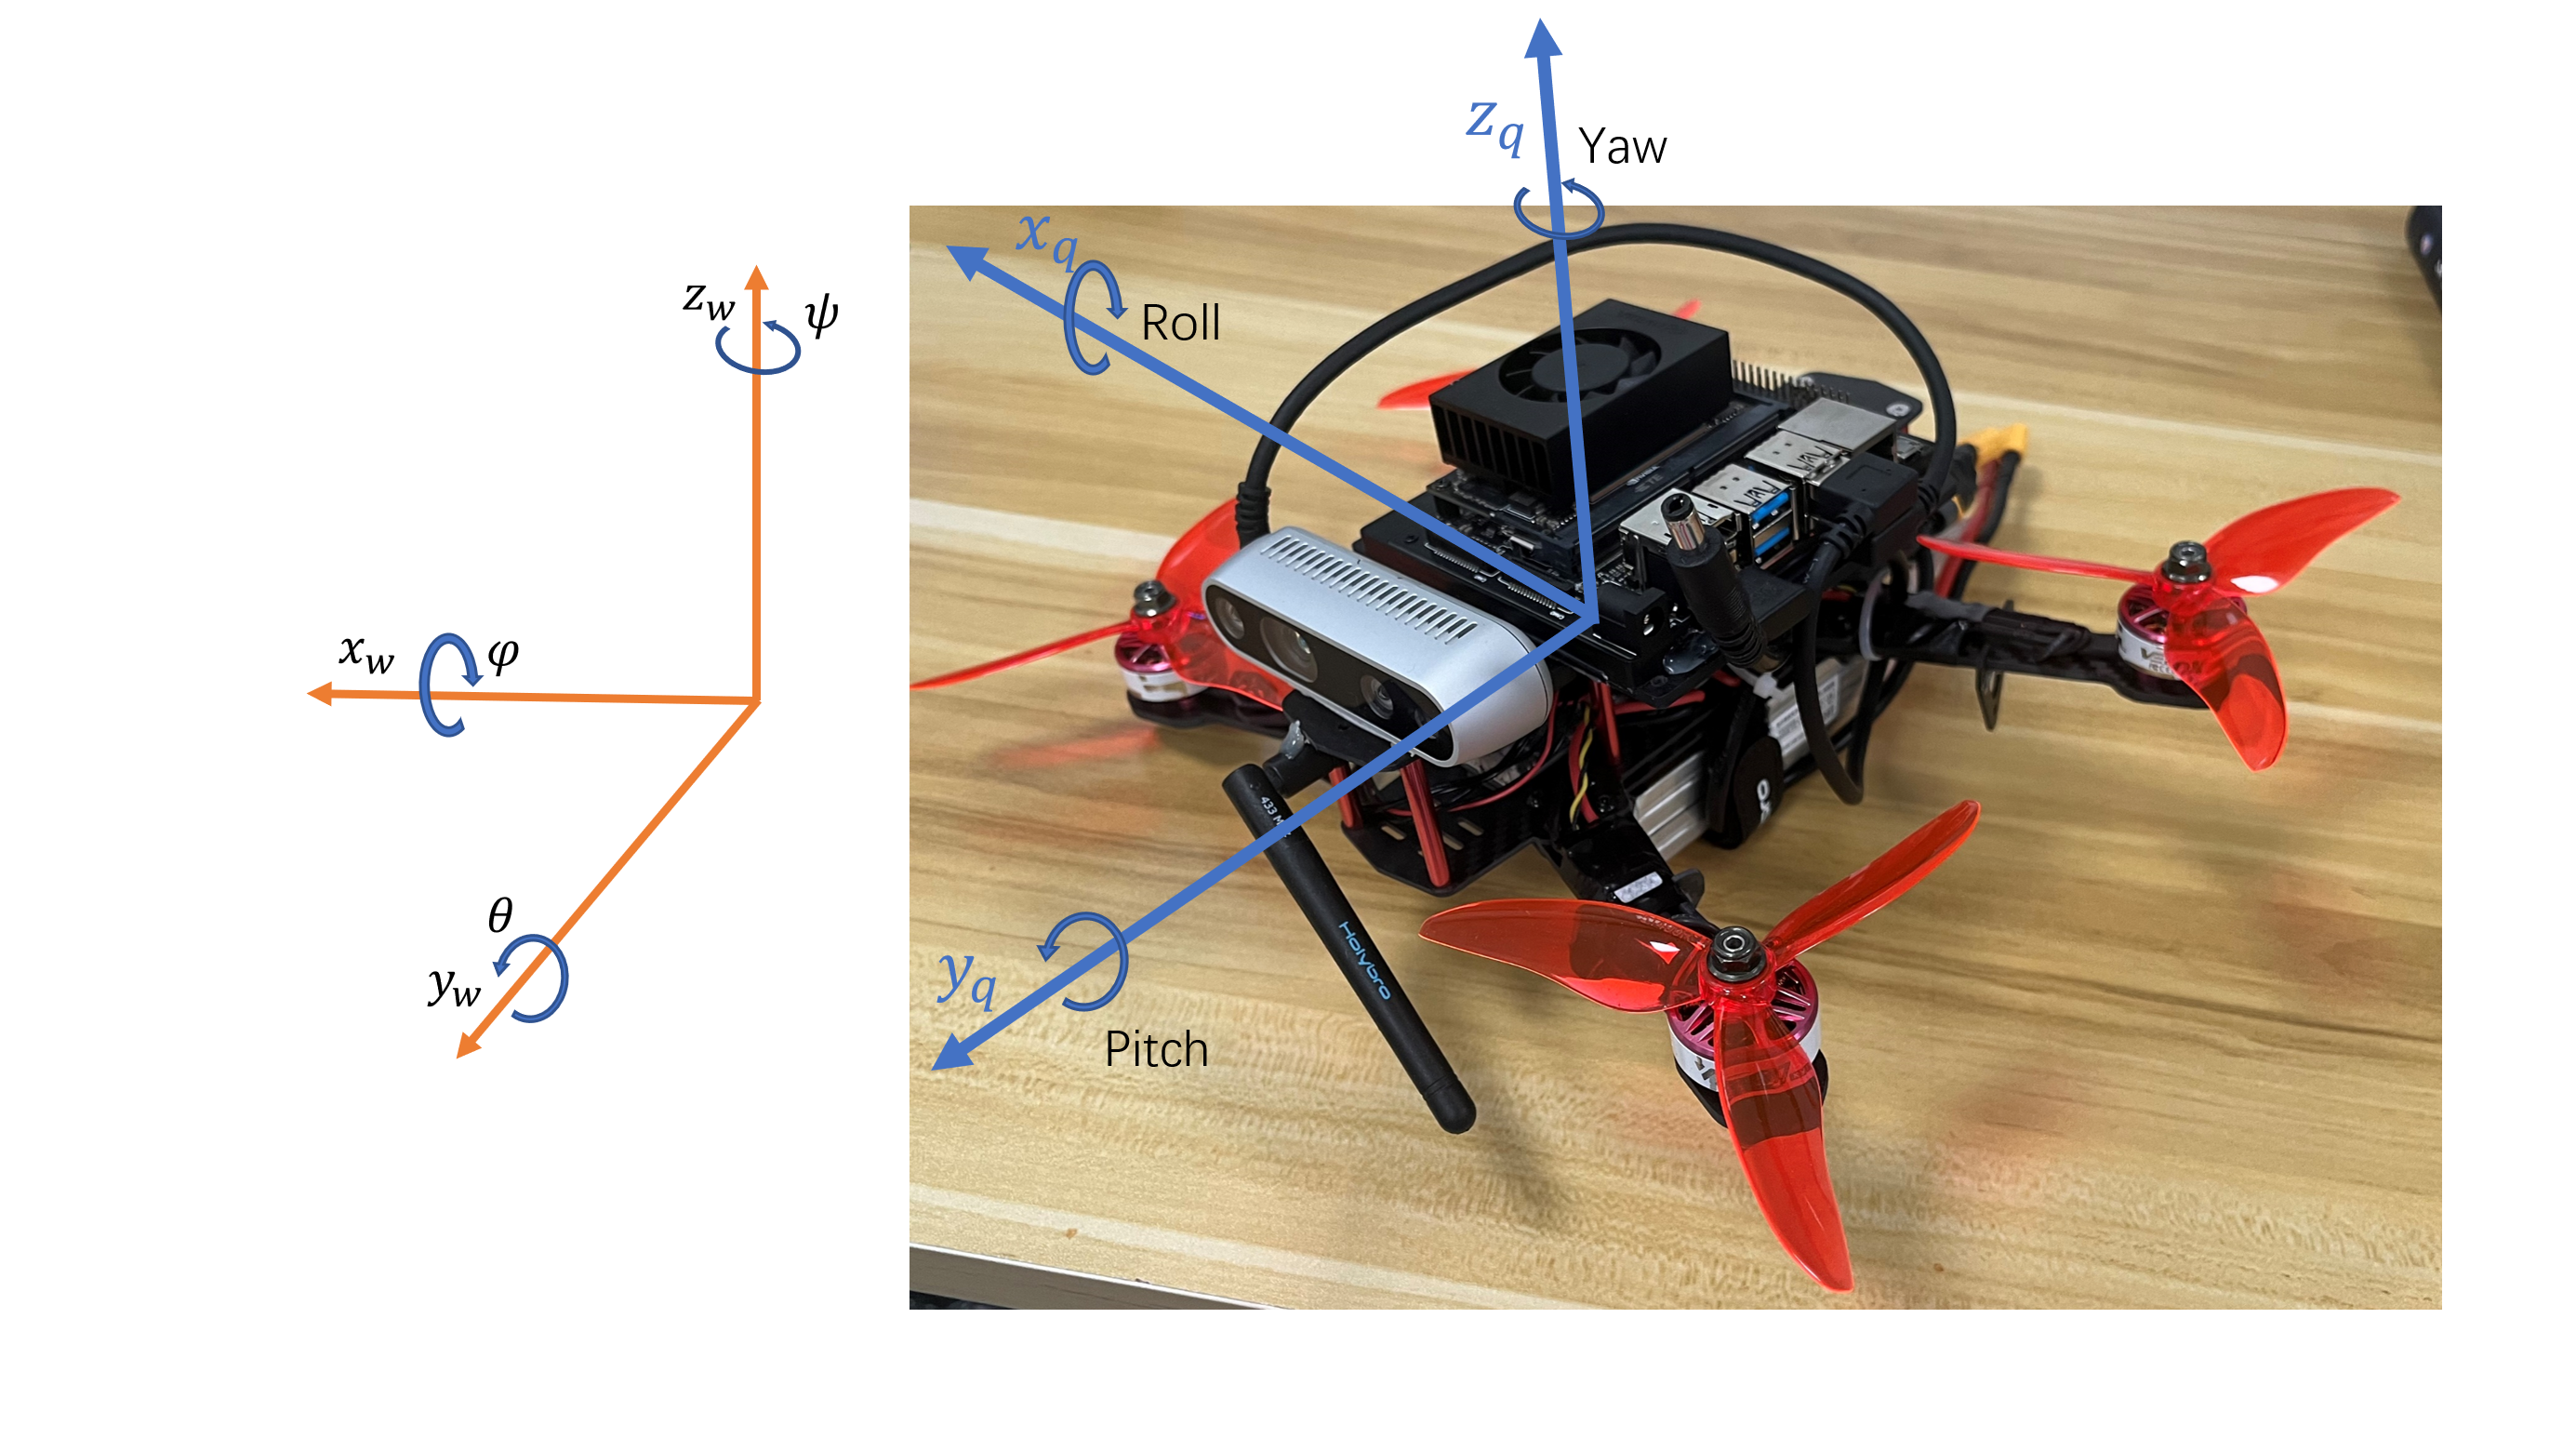
\includegraphics[width=0.7\textwidth]{coordinate.png}
      \caption{坐标系定义}
      \label{fig:1}
    \end{figure}
    首先是根据牛顿第二定律的质点动力学,由于旋翼的轴都垂直于机身平面,因此在机身坐标系下合力$f$永远垂直向下。

  \begin{equation}
    \dot x=v
  \end{equation}

  \begin{equation}
    -R \begin{bmatrix} 0\\ 0\\ f \end{bmatrix}+\begin{bmatrix} 0\\ 0\\ mg\end{bmatrix}=m \dot v 
    \label{equ:a}
  \end{equation}

    然后是刚体姿态动力学,为了表示形式的简洁以及工程实际的方便,位置和速度表示在地面系下,而角速度表示在
    机身坐标系下,因此刚体动力学方程还要加入补偿的$\omega \times J \omega$项:
  \begin{equation}
    M=J \dot\omega +\omega \times J \omega
    \label{equ:M}
  \end{equation}

    部分文献的建模中还会加入电机的陀螺力矩\cite{quanbook},$M_{gyro}=J_{rotor} \omega_{rotor} \times \omega$。 
    但出于多方面的考虑本文的模型中没有加入这一项。首先,由于控制的分层架构,在工程实现中要实时地得到电机转速  并不容易;其次,由叉乘性质可以发现,在电机转矩发生能力较弱的z轴上,陀螺力矩为$0$,其他两个方向上经过估算,
    与电机能提供的滚转俯仰力矩相比很小,完全可以当作干扰去克服;最后,省略这一项可以方便后面的理论推导。

最后是旋转矩阵导数和角速度的关系:
  \begin{equation}
    \dot R=R\Omega
    \label{equ:dotR}
  \end{equation}

\begin{proof}
  设在机身参考系下有一静止的单位向量 $r_0$ ,不妨把 $r_0$ 当作机头的方向向量,它与机体参考系固连,
  因此不随时间变化,是一个常值。其在世界坐标系下的坐标表示为 $r$ 
  $$r=R \cdot r_0$$
  
  两边对时间求导,由于 $r_0$ 是常值:
  \begin{equation}
    \dot r= \dot R \cdot r_0
    \label{equ:1}
  \end{equation}
  由于$r$是单位向量长度不变:
  \begin{equation}
    \dot r=R \omega \times r
    \label{equ:2}
  \end{equation}
  联立\ref{equ:1}  \ref{equ:2},由叉乘的分配律$A(b\times c)=(Ab)\times (Ac)$
  $$(R\omega)\times(Rr_0)=\dot R r_0$$
  $$\Rightarrow R(\omega \times r_0)=R\Omega r_0=\dot R r_0$$
  因为$r_0$任意:
  $$\Rightarrow \dot R=R \Omega'$$

\end{proof}

\subsection{动力分配}
上一节得到了从输入力和力矩到机身加速度和角加速度的关系,这一节将讨论如何从预期电机转速得到输入力和力矩。

计算单个旋翼产生的推力产生的推力和偏航力矩涉及到复杂的空气动力学,但也可以近似与转速平方成正比\cite{minimumsnap},即$f_i=k_F \omega_i^2,M_i=k_M \omega_i^2$。在正常工况的范围内,拟合较好。那么同一个旋翼产生的推力和偏航力矩就是正比关系,可以写作$M_i=c_{\tau f}f_i$。由于桨叶旋转会产生反方向力矩这一特性,如果无人机的四个旋翼全部顺时针旋转,这就会使得无人机在悬停时顺时针自转,并且无法通过控制反方向自转,逆时针同理。因此需要将无人机的桨叶配置成两正两反,对角的为一组,这样就能对消偏航力矩。在实践中,系数$c_{\tau f}$往往会非常小,这会使得控制偏航角变得困难,因有些无人机在设计时会给电机轴与机身垂直方向留出$3\sim5^\circ$的倾角,以便于改变偏航力矩。

在无人机的四个旋翼都竖直向下的情况下,无法产生水平方向的力,因此能产生的力的效果可以只用\ref{equ:trans}中等号左侧的四个参数就能表示。而旋翼的数量也是四个,这就使得动力分配变成了一一映射。分配矩阵是$4\times 4$ 的可逆方阵。
\begin{equation}
  \begin{bmatrix}
    f \\
    M_1 \\
     M_2\\M_3
    \end{bmatrix}=\begin{bmatrix}
    1 &1  & 1 & 1 \\
    0 & -d & 0 & d \\
    d & 0 & -d & 0 \\
    -c_{\tau f} & c_{\tau f} & -c_{\tau f} & c_{\tau f} \\
    \end{bmatrix}\begin{bmatrix}
     f_1\\
    f_2 \\
     f_3\\f_4
    \end{bmatrix}   
    \label{equ:trans}
\end{equation}

在得到每个旋翼的期望推力后,可以通过平方正比的关系解出期望转速,
电机速度闭环?好像不是,就是pwm开环,具体还要去看px4代码,先跳过

在仿真中,转速动态近似为一阶惯性环节,不考虑电调之类
先跳过



\section{高阶全驱系统理论}

高阶全驱(high-order fully actuated,HOFA)系统理论\cite{duan1},是由段广仁院士提出并完善为成体系的理论,为控制系统,尤其是处理非线性动态系统提供了新的视角。这一理论将卡尔曼提出的传统的一阶系统方法扩展到高阶情况,其中系统由二阶或更高阶的微分方程描述。大多数由基本物理定律建模的物理系统,比如牛顿第二定律、刚体动力学欧拉方程和基尔霍夫定律,自然表现为二阶系统。因此,HOFA系统理论提供了一种更自然和直接的方法来理解和控制这些系统,而不用将原本的高阶方程升维降阶到一阶的状态空间范畴里再设计控制算法。

\subsection*{关键概念}

\begin{itemize}
    \item \textbf{定义:}HOFA系统的特点是它们能够通过外部输入直接控制每个状态变量,这一特性基于全驱动属性。这个属性允许消除复杂的非线性动力学,简化控制设计并提高系统性能。
    
    \item \textbf{HOFA模型控制:}HOFA理论的一个核心概念是全驱动概念,这一概念从根本上改变了控制设计的方法。与最适合状态响应分析的状态空间表示不同,HOFA模型在控制应用中表现出色,为控制器设计提供了一条直接的路径。
    
    \item \textbf{控制设计:}HOFA方法在将系统表示为HOFA模型后,即可立即设计控制器。即使对于具有复杂非线性的系统,该模型也有效地线性化了控制过程,通过利用全驱动结构。
\end{itemize}

\subsection{应用与影响}

HOFA系统理论在机器人技术、航空航天和精密制造等多个领域有着广泛的应用。通过提供更直观和有效的控制设计方法,HOFA系统有潜力彻底改变我们分析、设计和实现控制系统的方式,以应对高阶和非线性动态。

\subsection{结论}

高阶全驱系统理论的发展标志着控制系统理论的重大进步。它不仅丰富了我们对复杂系统的理解,还提供了应对非线性和高阶动态挑战的实用工具。HOFA方法为控制系统设计提供了增强的能力,为各种工程领域的研究和应用开辟了新的途径。



% !TeX root = ../main.tex
\chapter{理论设计}  
由于四旋翼的推力方向只能向下,因此无法在不倾斜的情况下获得水平方向的推力从而改变水平位置。因此刚体的六个自由度无法同时被控制,使得四旋翼欠驱动,输入的维度是4,所以能直接控制的状态维度也是4。虽然四旋翼整体并不满足高阶全驱系统理论的要求,但是姿态环的三个自由度是全驱的,这从式(\ref{equ:M})(\ref{equ:dotR})可以清楚得看到。

四旋翼的控制分为姿态环和位置环两部分。从物理原理角度,分模态讨论,水平面内的飞行是对称的,以向前飞为例,需要机身先向前倾斜才能获得向前的分力。因此姿态的变化先于位置的变化,在实践中,姿态环的控制频率也远大于位置环。姿态环的动力学方程涉及到更强的非线性,并且姿态环一旦能迅速地达到期望值,位置控制也就水到渠成,因此四旋翼的控制中姿态环的重要性和难度都高于位置环。

\section{姿态控制}

\subsection*{误差定义}
姿态控制采用基于高阶全驱系统理论的方法,那么首先就需要定义一个合适的三维误差向量来描述当前姿态$R$到期望姿态$R_d$的差,使得控制输入矩阵可逆:
\begin{equation}
    e=(R_d^TR-R^TR_d)^\vee
\end{equation}

该误差定义不仅可以满足高阶全驱系统理论的要求,并且如式(\ref{error})所示,具有良好的物理意义。当$e\to 0$时,$\theta \to 0$,$R$与$R_d$重合,达到期望。

\subsection*{HOFA模型}
接下来需要对误差连续两次求导,使得方程中出现控制输入,也就是力矩$M$:
$$\begin{aligned}
    \dot e=&[(R_d^TR \Omega-\Omega_dR_d^TR)-(R_d^TR \Omega-\Omega_dR_d^TR)^T]^\vee\\
    =&[R_d^TR(\Omega-R^TR_d \Omega_dR_d^TR)-(R_d^TR(\Omega-R^TR_d \Omega_dR_d^TR))^T]^\vee \\
    =&[R' \hat e_\Omega  + \hat e_\Omega R'^T]^\vee
\end{aligned} $$
    定义
    $$R'=R_d^TR \quad e_\Omega=\omega -R^TR_d \omega_d$$
进一步求二阶导:
    $$\begin{aligned}
        \ddot e =& [(R' \hat e_\Omega \Omega + R'\dot \Omega -\Omega_d R' \hat e_\Omega -\dot \Omega_d R')-(R' \hat e_\Omega \Omega + R'\dot \Omega -\Omega_d R' \hat e_\Omega -\dot \Omega_d R')^T]^\vee\\
        =&[(R' \hat e_\Omega \Omega  -\Omega_d R' \hat e_\Omega -\dot \Omega_d R')-(R' \hat e_\Omega \Omega  -\Omega_d R' \hat e_\Omega -\dot \Omega_d R')^T]^\vee+[R'\dot \Omega-(R'\dot \Omega)^T]^\vee\\
        =&[(R' \hat e_\Omega \Omega  -\Omega_d R' \hat e_\Omega -\dot \Omega_d R')-(R' \hat e_\Omega \Omega  -\Omega_d R' \hat e_\Omega -\dot \Omega_d R')^T]^\vee\\
        & + \begin{Bmatrix}
        \begin{bmatrix}
        R'_{11} &R'_{12}  & R'_{13} \\
        R'_{21} & R'_{22} & R'_{23} \\
        R'_{31} & R'_{32} &R'_{33}  \\
        \end{bmatrix}&\begin{bmatrix}
        0 & -\dot\omega_3 &\dot\omega_2  \\
         \dot\omega_3& 0 &  -\dot\omega_1\\
         -\dot\omega_2&\dot\omega_1  & 0 \\
        \end{bmatrix}\end{Bmatrix}^\vee -\begin{Bmatrix}
        \begin{bmatrix}
        R'_{11} &R'_{12}  & R'_{13} \\
        R'_{21} & R'_{22} & R'_{23} \\
        R'_{31} & R'_{32} &R'_{33}  \\
        \end{bmatrix}&\begin{bmatrix}
        0 & -\dot\omega_3 &\dot\omega_2  \\
         \dot\omega_3& 0 &  -\dot\omega_1\\
         -\dot\omega_2&\dot\omega_1  & 0 \\
        \end{bmatrix}\end{Bmatrix}^{T\vee}\\
        =&[(R' \hat e_\Omega \Omega  -\Omega_d R' \hat e_\Omega -\dot \Omega_d R')-(R' \hat e_\Omega \Omega  -\Omega_d R' \hat e_\Omega -\dot \Omega_d R')^T]^\vee \\
        & +        \begin{bmatrix}
        R'_{22}+R'_{33} & -R'_{21} & -R'_{31} \\
         -R'_{12}& R'_{11}+R'_{33} & -R'_{32} \\
         -R'_{13}&- R'_{23} & R'_{11}+R'_{22} \\
        \end{bmatrix}\dot \omega\\
        =&A_d+R_B\dot \omega
        \end{aligned}  $$

        $$A_d=[(R' \hat e_\Omega \Omega  -\Omega_d R' \hat e_\Omega -\dot \Omega_d R')-(R' \hat e_\Omega \Omega  -\Omega_d R' \hat e_\Omega -\dot \Omega_d R')^T]^\vee$$

        $$R_B=\begin{bmatrix}
            R'_{22}+R'_{33} & -R'_{21} & -R'_{31} \\
             -R'_{12}& R'_{11}+R'_{33} & -R'_{32} \\
             -R'_{13}&- R'_{23} & R'_{11}+R'_{22} \\
            \end{bmatrix}$$
\textbf{$R_B$满秩}

    当$R_B$满秩时,符合高阶全驱的条件;不满秩时则短暂采用替补控制律。代入\ref{equ:M},得:
    $$\begin{aligned}
        \ddot e=&A_d+R_B J^{-1}(-\omega \times J\omega+M)\\
        =&A_d-B \omega\times J\omega +BM
        \end{aligned}$$
        $$B=R_BJ^{-1}$$

    高阶全驱系统建模完成,随即立刻可以设计控制算法。由于$B$可逆,令:
    $$M=-B^{-1} A_d+\omega \times J\omega +B^{-1}M^*$$
    使得
    $$\ddot e=M^*$$

    对于该补偿掉所有非线性部分的二阶积分器模型,得到状态空间表示下的方程:
    $$\dot x=\begin{bmatrix}
        0_{3\times 3} & I_{3\times 3} \\
        0_{3\times 3} & 0_{3\times 3}
    \end{bmatrix} x+\begin{bmatrix}
        0_{3\times 3} \\ I_{3\times 3}
    \end{bmatrix} M^* $$
    $$x=\begin{bmatrix}
        e \\ \dot e
    \end{bmatrix}$$
    在此基础上可以便利地采用任何线性系统控制器设计方法,采用LQR控制器,得到$M^*=-kx$

   $$ \begin{aligned}
        M=&-J R_B^{-1} [(R' \hat e_\Omega \Omega  -\Omega_d R' \hat e_\Omega -\dot \Omega_d R')-(R' \hat e_\Omega \Omega  -\Omega_d R' \hat e_\Omega -\dot \Omega_d R')^T]^\vee \\
         &+\omega \times J\omega + J R_B^{-1}(-kx)
    \end{aligned}$$

    \textbf{$R_B$不满秩}

    $R_B$不满秩时,上述高阶全驱方法就不在成立,但是不满秩的点在$\mathbb{R^{3 \times 3}}$是无处稠密的,因此在实验中几乎不会遇到。但是为了理论的完备,设置替补控制律\cite{Lee2010}:
    $$M=-k_R e_R-k_\omega e_\omega+\omega \times J \omega -J(\Omega R'^T \omega_d-R'^T \dot \omega_d) $$
    $$ e_R=\frac{1}{2} (R'-R'^T)^\vee $$
    这种控制律能保证指数收敛,参数$k_R,k_\omega$需要根据转动惯量调试后选定。
    \section{位置控制}
    在设计位置环的控制算法时,首先要结合期望偏航角生成期望姿态$R_d$作为姿态环的输入。然后,考虑到姿态环的高响应速度,其动态过程可以被忽略。这一假设进一步简化了位置环的动力学方程,使其也能被视作一个线性系统,仍然先采用LQR方法进行控制。

    
    \subsection{期望姿态生成}
    期望姿态$R_d$是由位置环输出以及期望偏航角生成的,它代表了要达到期望的位置所需的推力方向。由于无人机的推力只能垂直于机身平面,要到达期望的位置需要有指向该位置的力,因此要首先改变无人机姿态使其法线方向平行于期望推力方向,再结合外部输入的期望偏航角,就能得出期望的姿态\cite{Lee2010}。

    在本课题中,机头的指向即偏航角相对来说没有期望位置重要,且在姿态较大时,偏航角的意义实质上并不明确:偏航角如果是Z-Y-X欧拉角定义下的第一个转角,当后两个转角较大时,偏航角也就脱离了原本的物理意义。因此首先保证期望推力方向,将其设计成反馈加前馈的形式:
    $$f_{ideal}=k_x e_x+k_v e_v-mg \vec e_3+m a_d$$
    $$\vec b_{3d}=-\frac{f_{ideal}}{||f_{ideal}||}$$
    $$ e_x=x_d-x \quad e_v=v_d-v \quad \vec e_3=\begin{matrix}
        [0 & 0 & 1]
    \end{matrix}^T$$

    然后将期望偏航角产生的单位向量$\begin{matrix} [\cos{\psi_d} & \sin{\psi_d} & 0]  \end{matrix}^T$投影到垂直于$b_{3d}$的平面上,就能得到期望姿态$R_d= \begin{matrix} [ \vec b_{2d}\times \vec b_{3d} &\vec b_{2d} & \vec b_{3d}] \end{matrix}$,$\vec b_{2d}=\vec b_{3d} \times \vec b_{1d}$,如图 \ref{fig:2}。
    \begin{figure}[!h]
        \centering
        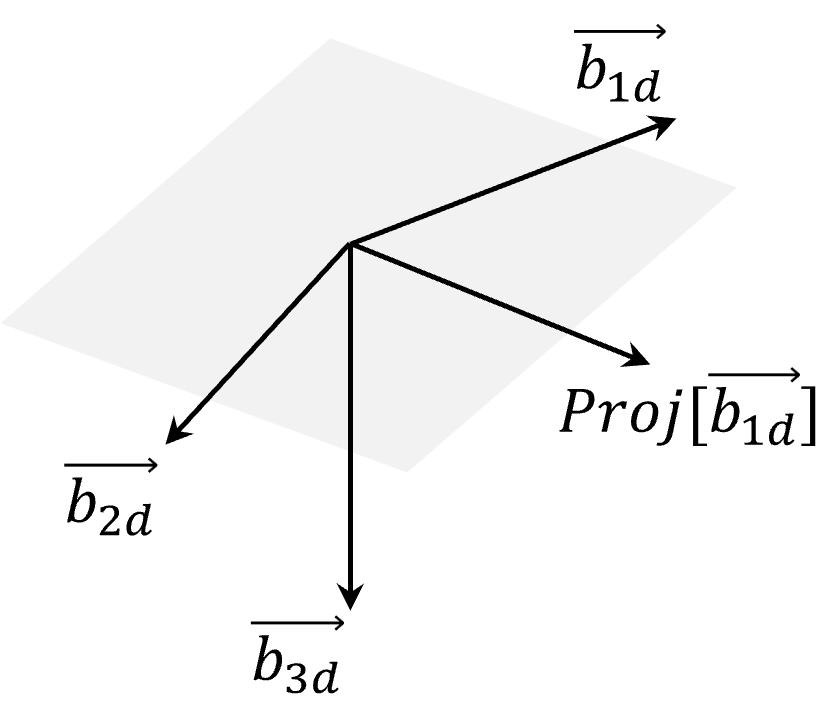
\includegraphics[width=0.3\textwidth]{desired R.png}
        \caption{期望姿态定义}
        \label{fig:2}
      \end{figure}

      \subsection{推力控制律}
      以上计算得到的$f_{ideal}$完全没有考虑姿态动态过程,由于$R$不可能瞬间收敛到$R_d$,当姿态尚未收敛时,推力的控制指令应当为$f_{ideal}$在当前姿态推力方向上的投影,否则会在错误的方向上投入过多的力分量:
      $$f=f_{ideal}\cdot R e_3$$
      接下来需要得出控制律$k_x \quad k_v$,当姿态$R$能迅速收敛到$R_d$时,动力学方程\ref{equ:a}退化为:
      $$m \dot v=mge_3-f$$

      那么位置控制环节就变成了简单的线性系统,可以写作六阶状态空间表示
      $$\dot x=\begin{bmatrix}
        0_{3\times 3} & I_{3\times 3} \\
        0_{3\times 3} & 0_{3\times 3}
    \end{bmatrix} x+\begin{bmatrix}
        0_{3\times 3} \\ \frac{1}{m} I_{3\times 3}
    \end{bmatrix} f +\begin{bmatrix}
        0_{3 \times 1} \\ a_d-g \vec e_3 
    \end{bmatrix}$$
    $$x=\begin{bmatrix}
        x_d -x \\ v_d -v
    \end{bmatrix}$$
      将$f$写作补偿掉前馈的形式:$f=f^*-mg \vec e_3 +m a_d$。接下来就可以运用LQR方法得到控制律$f^*=-kx$。

    $f^*$的控制律并不是四旋翼运动控制的关键,只要期望姿态生成合理并且姿态环能迅速收敛,位置环的控制难度很低。因此在后面的ros仿真以及实机实验中,位置环将不对PX4的代码做更改(PX4的位置环控制算法事实上完全包含了上述算法,将I和D置0即可退化为本文中的方法),以避免架构上不必要的麻烦。

% !TeX root = ../main.tex
\chapter{仿真实验}
仿真实验分为三步,首先在Matlab中基于s-function和simulink仿真,验证控制算法的性能;然后在ros框架下,基于PX4固件,修改其运动控制部分的代码,在gazebo中进行软件在环仿真(SITL,software in the loop);接着,将修改后的PX4固件烧写到pixhawk飞控板中,进行硬件在环仿真(HITL,hardware in the loop),而这个版本的固件也可以直接用于后续的实机实验。
\section{Matlab仿真}
我们在Simulink环境下构建了一个综合仿真模型,该模型不仅包含了刚体动力学和电机动态,还通过s-function实现了姿态环和位置环分离的双环控制器设计。这种设计使得后续的数据分析和研究工作能够更为便捷、高效。

为了能直观地体现性能,我们设计了一个“8”字型轨迹,如图\ref{fig:8}:
$$x_d = \begin{matrix}[3\sin(\frac{t}{2}), & 3\cos(\frac{t}{2})\sin(\frac{t}{3}), &-0.1t]\end{matrix}
\quad
\psi_d=0.01t$$

\begin{figure}[!h]
  \centering
  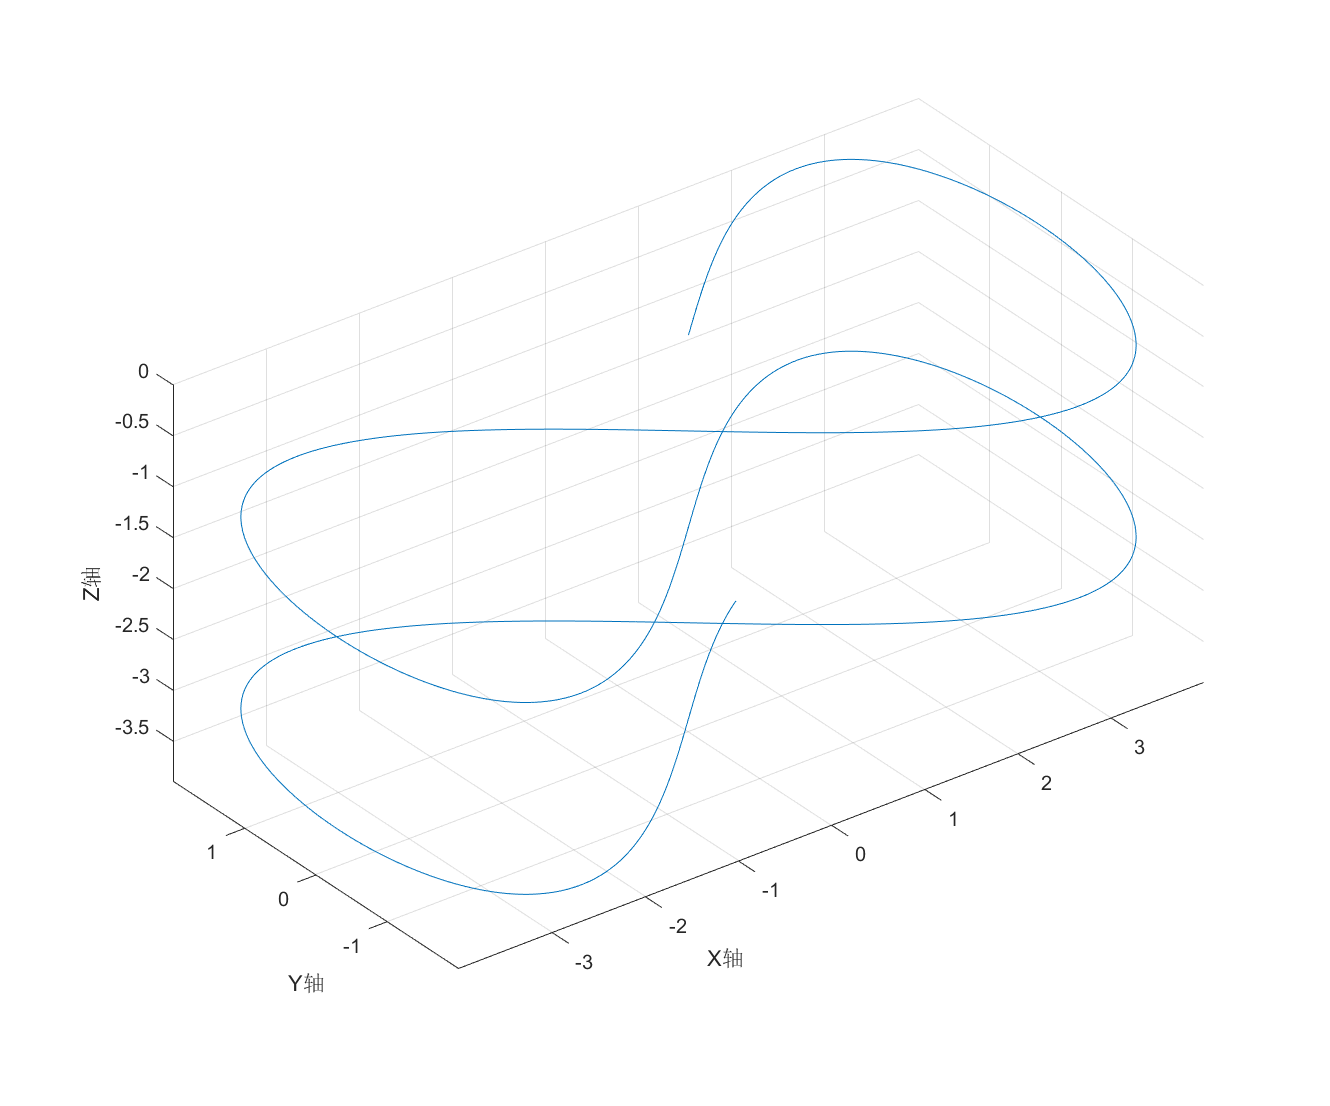
\includegraphics[width=0.5\textwidth]{88.png}
  \caption{高度匀速上升的“8”字型轨迹(北-东-地坐标系下,地面以上Z轴为负数)}
  \label{fig:8}
\end{figure}

为了全面体现控制算法的跟踪性能,我们并没有对轨迹做特殊的平滑处理,轨迹的导数存在间断点使得高阶导数无穷大,这可以考验无人机在现实中的抗扰性能。为了模拟起飞和悬停,第一秒内轨迹保持在原点不动,否则仿真就会等同在空中释放电机无转速的无人机。


  无人机的刚体动力学部分由simulink中自带的“6DOF block”解决,避免了$SO(3)$群差分近似后单位化的困难。该模块会对外部输入的力和力矩做出反应,返回所需的速度、位置、姿态、角速度等信息。

  电机部分,转速的动态由一阶惯性环节表示,根据所选电机型号时间常数$\tau=0.01s$。
  姿态控制器和位置控制器分开由两个s-function实现,重力由单独的模块输入到“6DOF block”。
  \begin{figure}[!h]
    \centering
    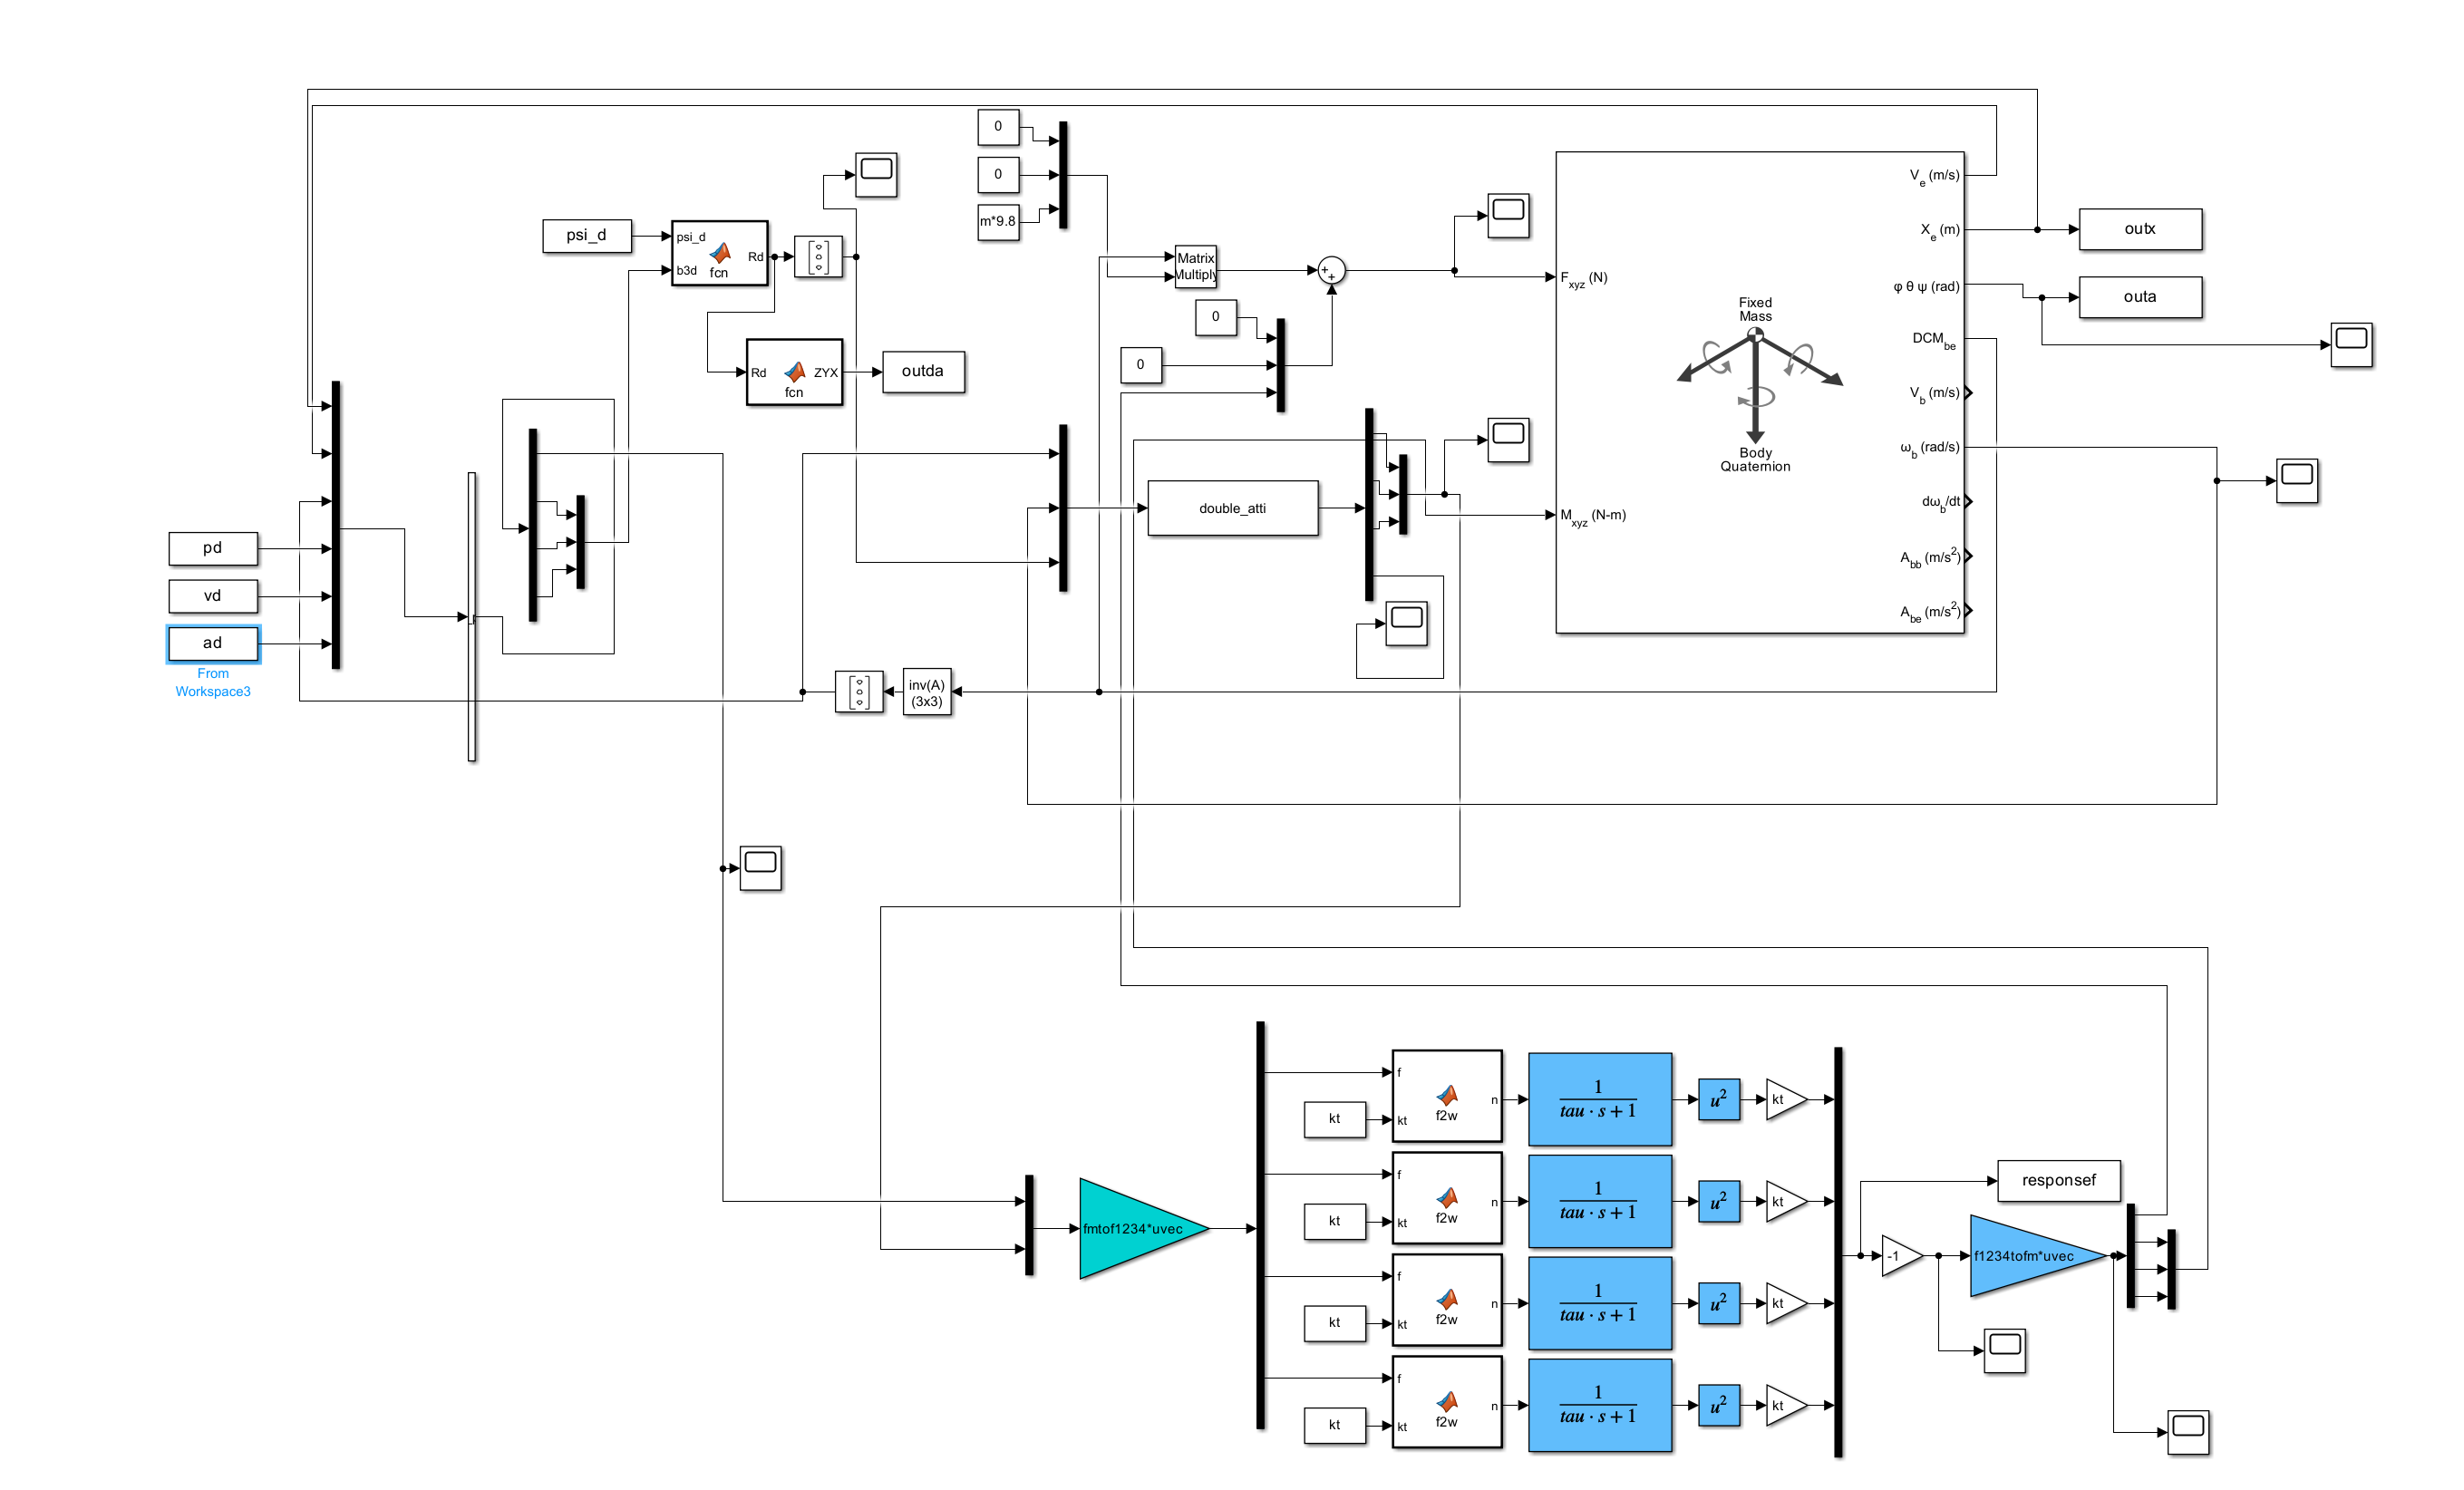
\includegraphics[width=0.9\textwidth]{sim.png}
    \caption{simulink仿真连线图}
    \label{fig:sim}
  \end{figure}

  四旋翼无人机的参数由测量和理论计算共同得到:
  $$m=0.8kg \quad d=0.125m \quad J=\begin{bmatrix}
    0.0024   &      0  &       0\\
    0 &   0.0025      &   0\\
    0  &       0   & 0.0041
  \end{bmatrix}kg m^2$$

  电机参数由厂家数据得到:
  $$k_t=2.03\times 10^{-8} \quad 
  \tau=0.01s \quad
  c_{\tau f}=8\times 10^{-3}$$

  选择替补姿态控制律:
  $$k_R=0.881 \quad k_\omega=0.254$$

  由于位置环和姿态环补偿后得到的线性系统A矩阵完全一致,因此选择相同的LQR权重矩阵:
  $$Q=\begin{bmatrix}
    3&0&0&0&0&0\\
    0&3&0&0&0&0\\
    0&0&3&0&0&0\\
    0&0&0&1&0&0\\
    0&0&0&0&1&0\\
    0&0&0&0&0&1\\
  \end{bmatrix} \quad R=\begin{bmatrix}
    0.1 &0 &0\\
    0 &0.1 &0\\
    0 &0 &0.1\\
  \end{bmatrix}$$

  初始位姿:
  $$x(0)=[0,0,0],\quad v(0)=[0,0,0]$$
  $$R(0)=I , \quad \omega(0)=[0,0,0]$$

  按照上述参数,在matlab中用0.005s的控制周期运行仿真,得到结果如图\ref{fig:result-x},\ref{fig:result-angle},\ref{fig:result-f}:
  \begin{figure}[h]
    \centering
    \begin{minipage}[c]{0.33\textwidth}
      \centering
      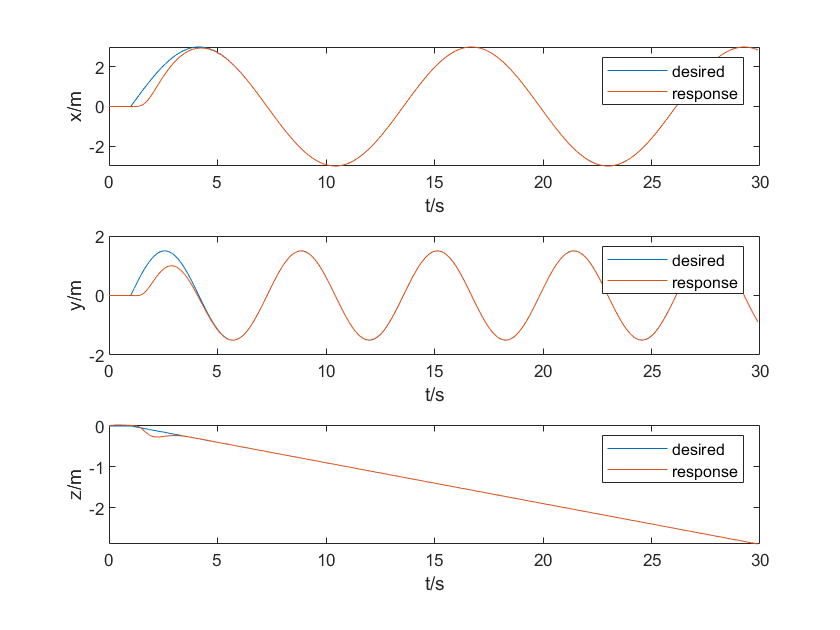
\includegraphics[width=0.95\linewidth]{result-x.png}
      \caption{位置跟踪效果}
      \label{fig:result-x}
    \end{minipage} \hfill
    \begin{minipage}[c]{0.33\textwidth}
      \centering
      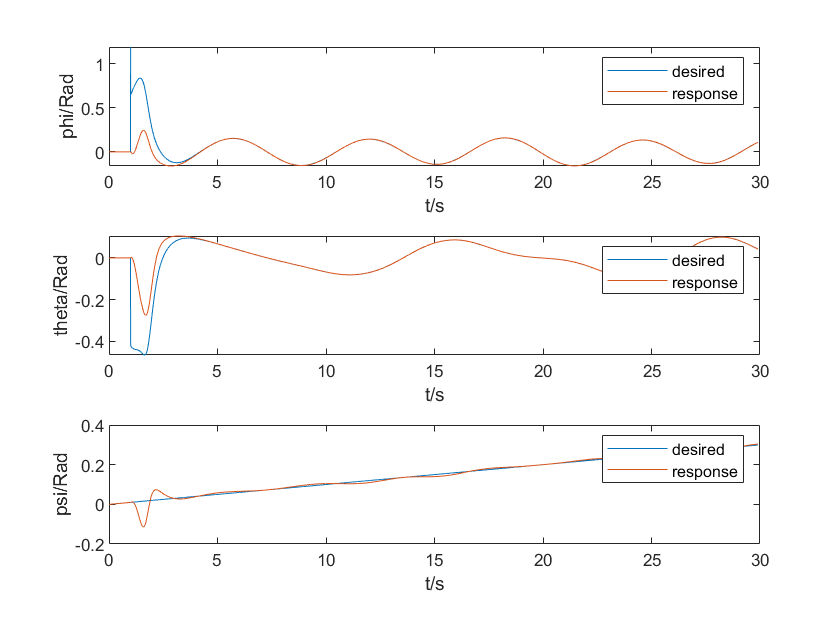
\includegraphics[width=0.95\linewidth]{result-angle.png}
      \caption{角度跟踪效果}
      \label{fig:result-angle}
    \end{minipage}\hfill
      \begin{minipage}[c]{0.33\textwidth}
        \centering
        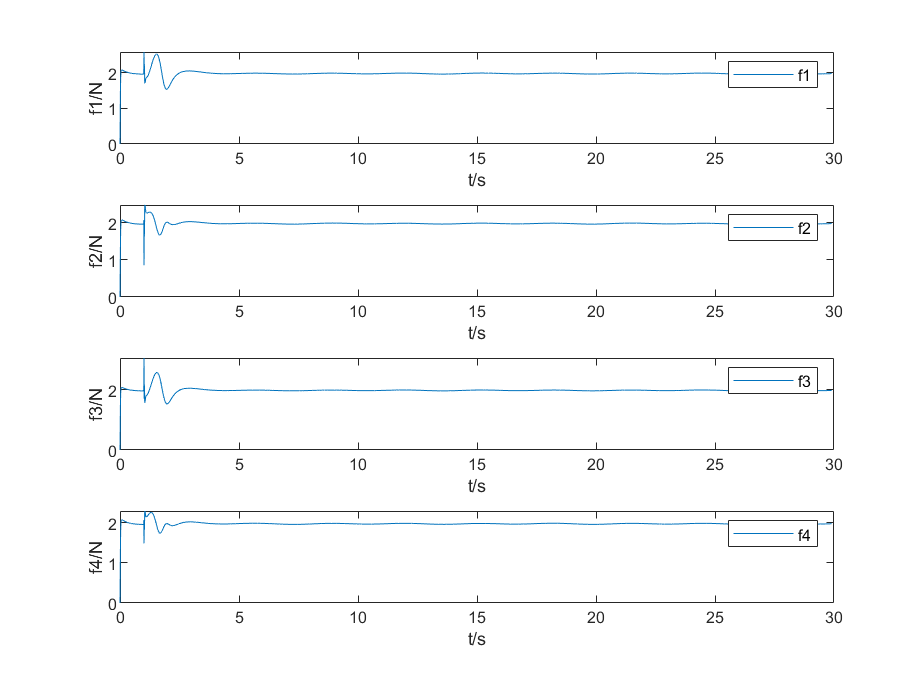
\includegraphics[width=0.95\linewidth]{result-f.png}
        \caption{四个电机输出的力}
        \label{fig:result-f}
    \end{minipage}
    \end{figure}

  从以上图中可以看到本控制算法可以很好地跟踪这种有较大姿态机动的轨迹,只是由于轨迹在起始时存在阶跃,导致无人机在阶跃处需要一定的动态过程才能跟踪上。但是在实际的飞行任务中,在轨迹规划层面就需要对轨迹做光滑处理。为了避免出现执行器饱和的情况,在仿真中我们根据无人机的实际情况和电机所能输出的最大升力,设置了控制器输出力和力矩的上限。

  \pagebreak
  
  三维空间下的轨迹跟踪情况如图\ref{fig:result-3d}

  可以看到在起始的阶跃之后,跟踪效果都十分完美,为了量化地展示跟踪效果,我们提出了平均距离误差和平均偏航角误差:
  $$e_d=\frac{\sum_0^{T}||x-x_d||}{T} \quad e_\psi=e_d=\frac{\sum_0^{T}|\psi-\psi_d|}{T}$$

  误差曲线如图\ref{fig:result-e}
 

  \begin{figure}[h]
    \centering
       \begin{minipage}[c]{0.45\textwidth}
        \centering
        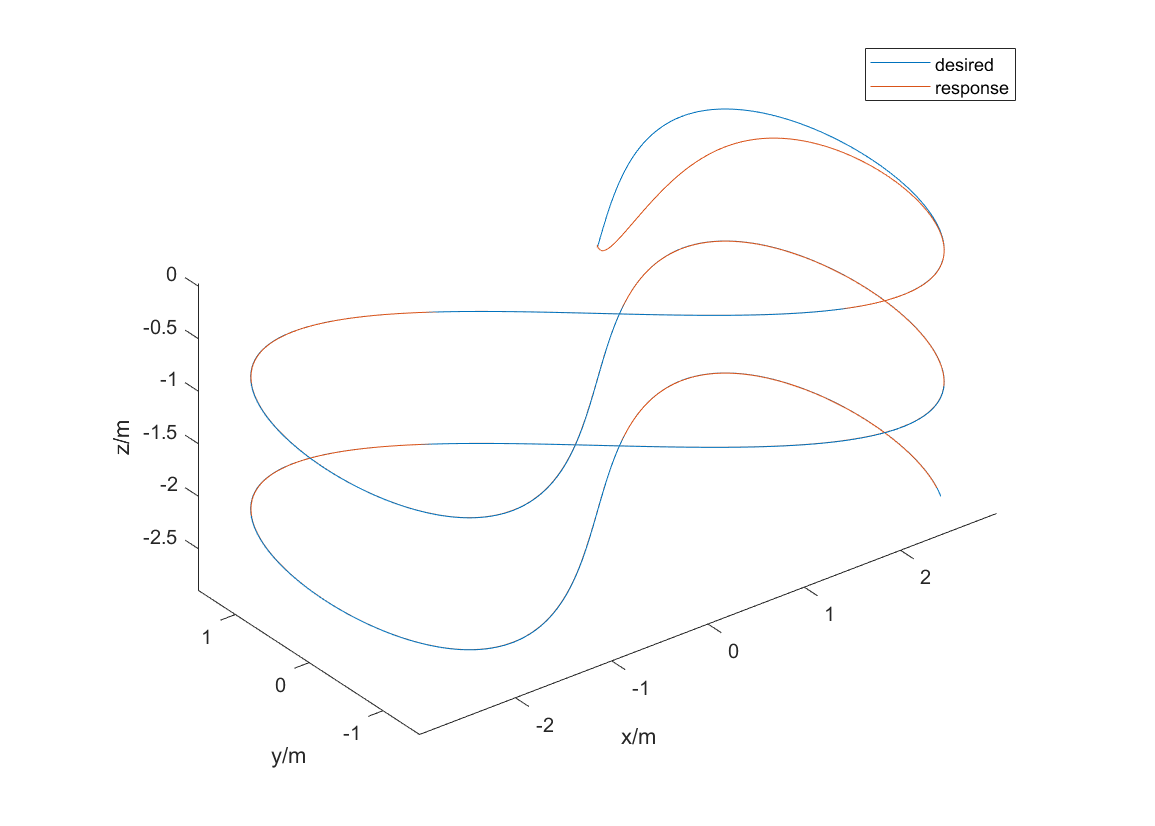
\includegraphics[width=0.9\textwidth]{result-3d.png}
        \caption{三维空间下的轨迹跟踪情况}
        \label{fig:result-3d}
     \end{minipage}%
       \begin{minipage}[c]{0.45\textwidth}
        \centering
        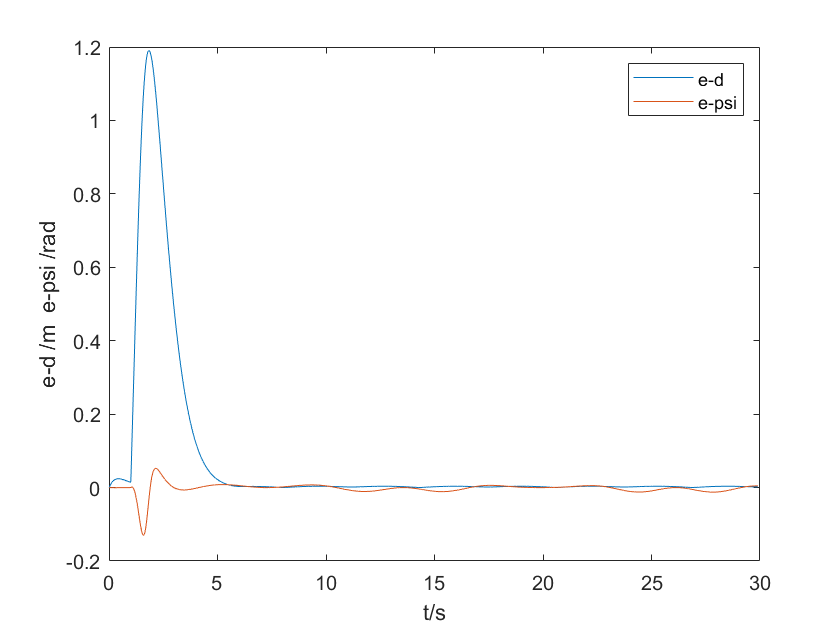
\includegraphics[width=0.9\textwidth]{result-e.png}
        \caption{平均距离误差和平均偏航角误差}
        \label{fig:result-e}
     \end{minipage}
   \end{figure}

   为了体现本控制方法的优越性,设置对照组,与\cite{Lee2010}中也就是上文所说的替补姿态控制律对比(位置环相同):
   
  \begin{figure}[h]
    \centering
    \begin{minipage}[c]{0.33\textwidth}
      \centering
      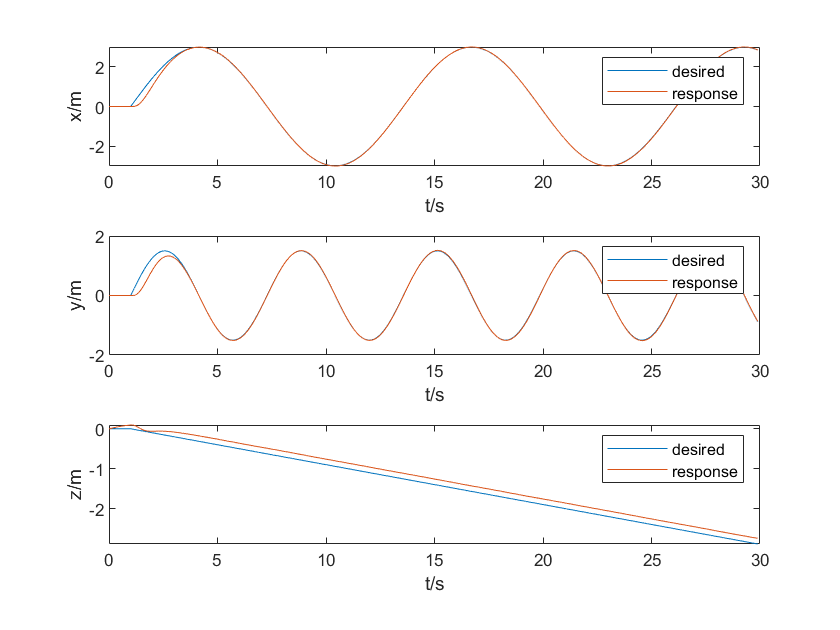
\includegraphics[width=0.95\linewidth]{com-x.png}
      \caption{对照组位置跟踪效果}
      \label{fig:com-x}
    \end{minipage} \hfill
    \begin{minipage}[c]{0.33\textwidth}
      \centering
      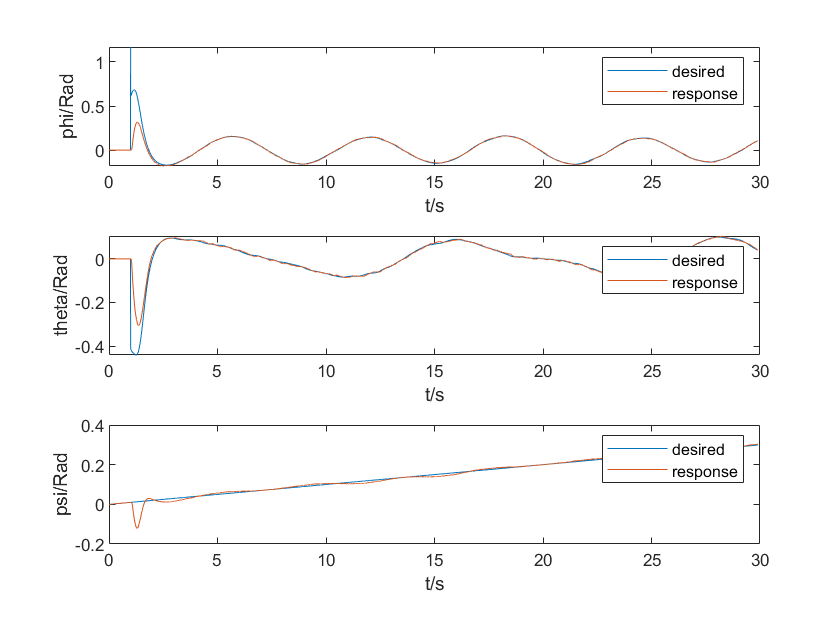
\includegraphics[width=0.95\linewidth]{com-angle.png}
      \caption{对照组角度跟踪效果}
      \label{fig:com-angle}
    \end{minipage}\hfill
      \begin{minipage}[c]{0.33\textwidth}
        \centering
        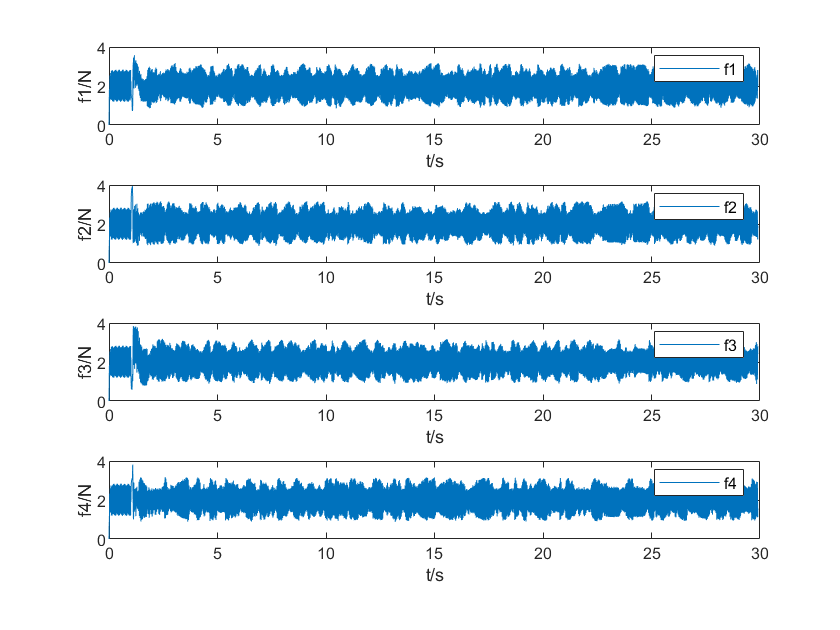
\includegraphics[width=0.95\linewidth]{com-f.png}
        \caption{对照组四个电机输出的力}
        \label{fig:com-f}
    \end{minipage}
    \end{figure}

    \begin{figure}[h]
      \centering
         \begin{minipage}[c]{0.45\textwidth}
          \centering
          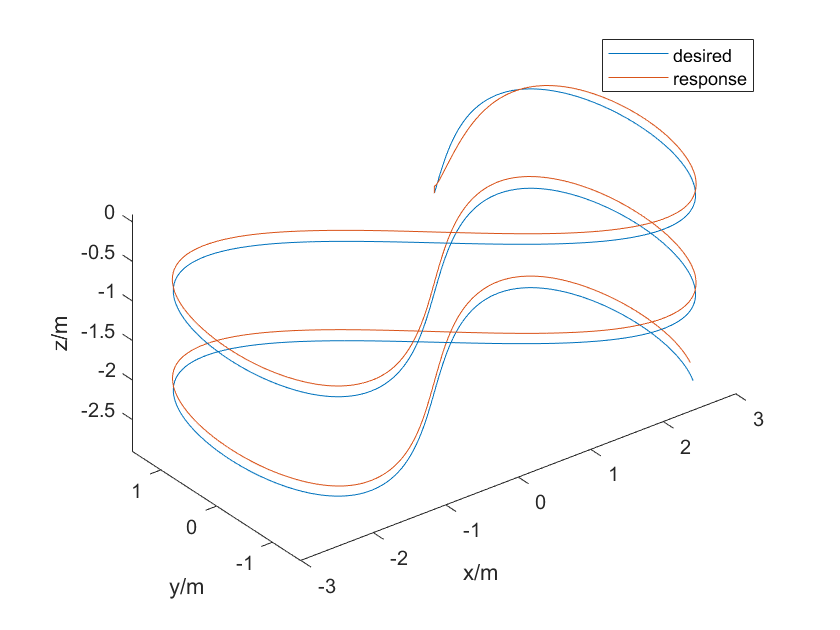
\includegraphics[width=0.9\textwidth]{com-3d.png}
          \caption{对照组三维空间下的轨迹跟踪情况}
          \label{fig:com-3d}
       \end{minipage}%
         \begin{minipage}[c]{0.45\textwidth}
          \centering
          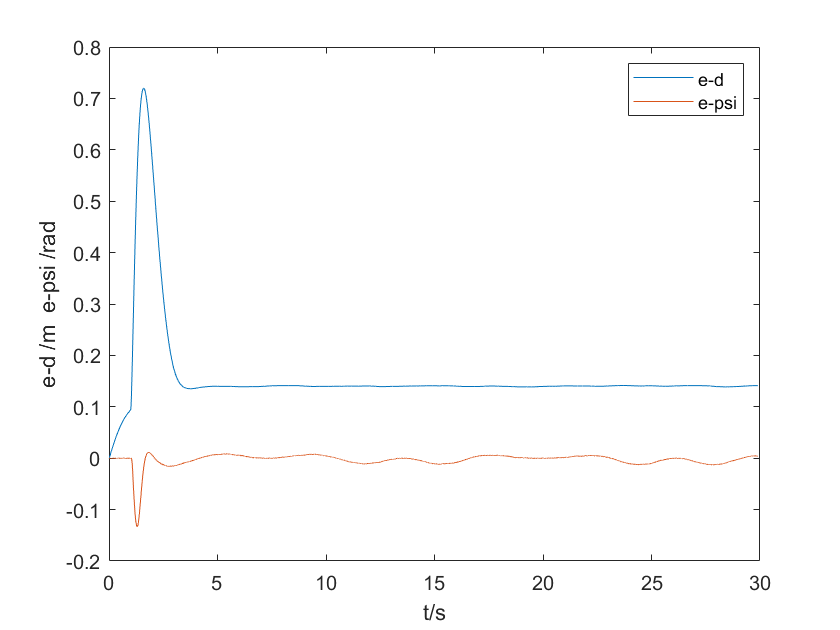
\includegraphics[width=0.9\textwidth]{com-e.png}
          \caption{对照组平均距离误差和平均偏航角误差}
          \label{fig:com-e}
       \end{minipage}
     \end{figure}

     从图\ref{fig:com-3d}中可以直观地看到其跟踪始终有误差未能弥合,在阶跃处同样需要一个动态过程。图\ref{fig:com-f}显示,其推力始终有剧烈抖动,这有可能是因为姿态环的参数调节欠缺。但这正体现了HOFA方法的优越性,相比于对照组的参数调节缺乏理论指导,只能根据经验多次尝试,HOFA方法能将非线性部分全部补偿掉,留下的线性系统对LQR参数并不敏感,权重矩阵并不需要精细地多次调解就能取得很好的控制效果。
     \begin{table}
      \centering
      \begin{tabular}{ccc}
          \toprule
          & 平均距离误差 & 平均偏航角误差 \\
          \midrule
          HOFA方法 & 0.0692 & 0.0072 \\
          对照组 & 0.1580 & 0.0065 \\
          \bottomrule
      \end{tabular}
      \caption{HOFA方法与对照组的平均误差对比}
  \end{table}

  量化的误差指标同样显示,在位置跟踪上,HOFA大幅领先于对照组。在偏航角误差的指标上,有小幅落后,但两者的误差都已经很小。

\section{软件在环仿真}
% !TeX root = ../main.tex
\chapter{实机实验}
仿真实验与实机实验同步进行,也可以分成三个阶段:首先是搭建飞行平台,使得无人机可以在室外的GPS定位下进行遥控飞行,并且其动力足以应对后续的载荷增加;然后是在室内动作捕捉(motion capture)的外部定位下进行遥控飞行和轨迹跟踪,此时无人机上搭载机载电脑(companion computer)来提供动捕位姿信息和控制指令,控制算法仍然是PX4的四环pid控制;最后,在得到改成高阶全驱控制方法的飞控固件后,将其烧写进飞控板中,完成室内的遥控飞行和轨迹跟踪。
\section{飞行平台搭建}
一架用于室外GPS下飞行的无人机的基本组成部分有机架、螺旋桨、电机、电子调速器(简称电调)、飞控、GPS接收器、遥控接收机、与地面站通信的sik电台或wifi热点和电池。而动力套件指的是其中的螺旋桨、电机和电调,它们合在一起决定一架无人机的动力性能。
\begin{figure}[h]
  \centering
  \begin{minipage}[c]{0.33\textwidth}
    \centering
    \includegraphics[width=0.95\linewidth]{GPS飞机.jpg}
  \end{minipage} \hfill
  \begin{minipage}[c]{0.33\textwidth}
    \centering
    \includegraphics[width=0.95\linewidth]{GPS侧面.jpg}
  \end{minipage}\hfill
    \begin{minipage}[c]{0.33\textwidth}
      \centering
      \includegraphics[width=0.95\linewidth]{GPS底部.jpg}
  \end{minipage}
  \caption{用于室外飞行的四旋翼无人机多角度照片}
  \end{figure}


在所有的部件中,除了与地面站的通信装置的功能会被机载电脑替代,以及GPS接收器不再需要之外,其他的部件都不会有更改,因此只要在第一阶段的实验中将其调试定型,就可以继续在后续的实验中使用。在这一阶段,由于飞控、GPS接收器、sik电台和遥控接收机都已经有完善的产品,使用只需要正确的连线和配置,并且对后续的研究没有太大的影响,因此不是我们研究的重点。

而动力套则不然,它的性能需要和无人机的载重相匹配,并且会体现在后续的建模和控制之中。动力套内部的三者之间也存在很强的耦合关系,需要互相适配:电调的输入是飞控的电机控制信号,根据协议的不同可以分为模拟的pwm信号和数字的dshot、oneshot等,经过调制向电机输出三相交流电。三相交流电的频率决定无刷电机的转速上限,但由于外部载荷、空气阻力、机械摩擦等阻力矩以及反电动势等阻力因素的存在,三相交流电需要有足够高的电压才能克服这些阻力因素使电机转速达到设定值。这样的逻辑意味着,在设定的转速不变时,电调不需要改变三相交流电的频率而只用改变电压去克服外部不断波动的负载。在选型时要注意电调能提供的最大电流要超过电机的最大电流,并且留有$5\sim 10A$的余量。螺旋桨和电机的型号也需要互相匹配,使空气阻力的负载和电机的扭矩互相适应。电机的产品说明中会有详细的油门量与电压、电流、力效等输出的表格,要保证电机能提供的拉力足够带起载荷,并且出于抗扰和稳定的需要,要留出足够大的余量。如图\ref{电机表}所示,在$60 \%$的油门量时,单个电机就能提供$913.8g$的升力,而后续搭载了机载电脑的无人机质量仅有$873.1g$,推重比达到了4.18 。
\begin{figure}[!h]
  \centering
  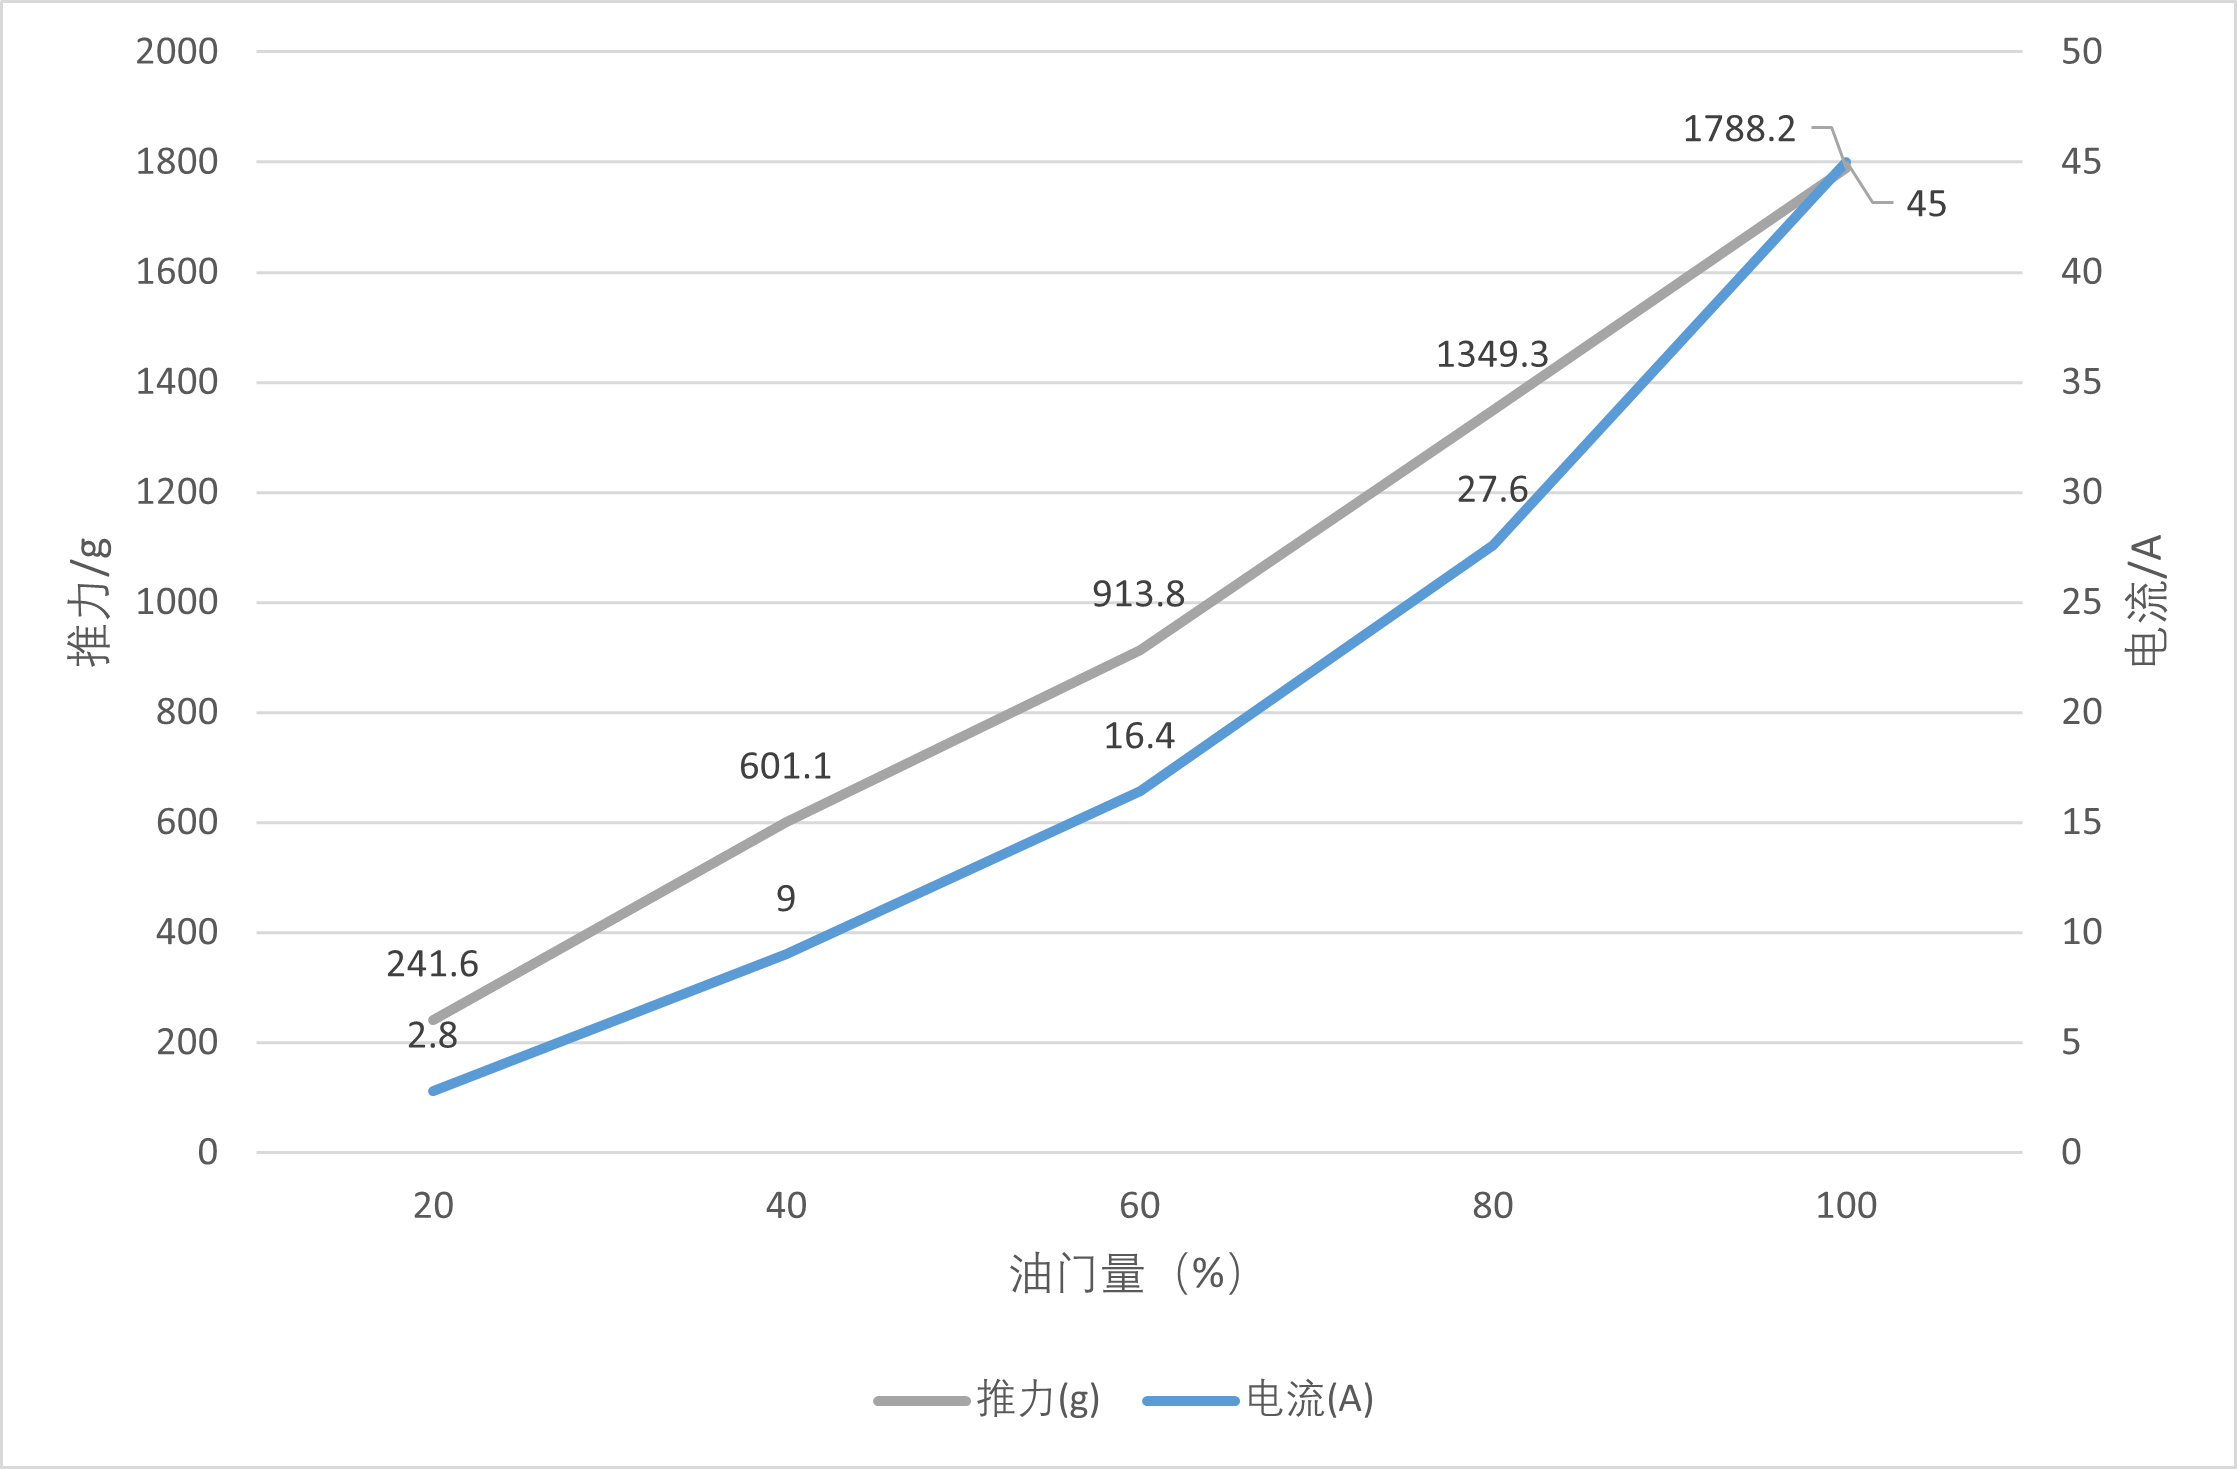
\includegraphics[width=0.7\textwidth]{电机表.png}
  \caption{Tmotor v2207 kv1950电机搭配51477-3螺旋桨 油门量与电流和推力关系图 \cite{Tmotor2023}}
  \label{电机表}
\end{figure}

在几番摸索后,考虑到后续的机载电脑等载荷需要有足够的安装位置,我们选择了holybro品牌的QAV250机架作为平台,以及配套的PM06电源及电调模块,TMOTOR v2207 kv1950电机和pixhawk 6c mini飞控。在装配和接线后,在QGroundControl地面站中对飞控烧写PX4 v1.14版本的固件,并进行传感器校正和遥控器设置。最后,在卫星信号良好的室外进行了遥控器控制下的飞行实验。无人机能够很好地执行遥控器发布的飞行指令,悬停稳定,前进后退自如,飞行效果如图 \ref{室外飞行}。

\begin{figure}[h]
  \centering
  \begin{minipage}[c]{0.33\textwidth}
    \centering
    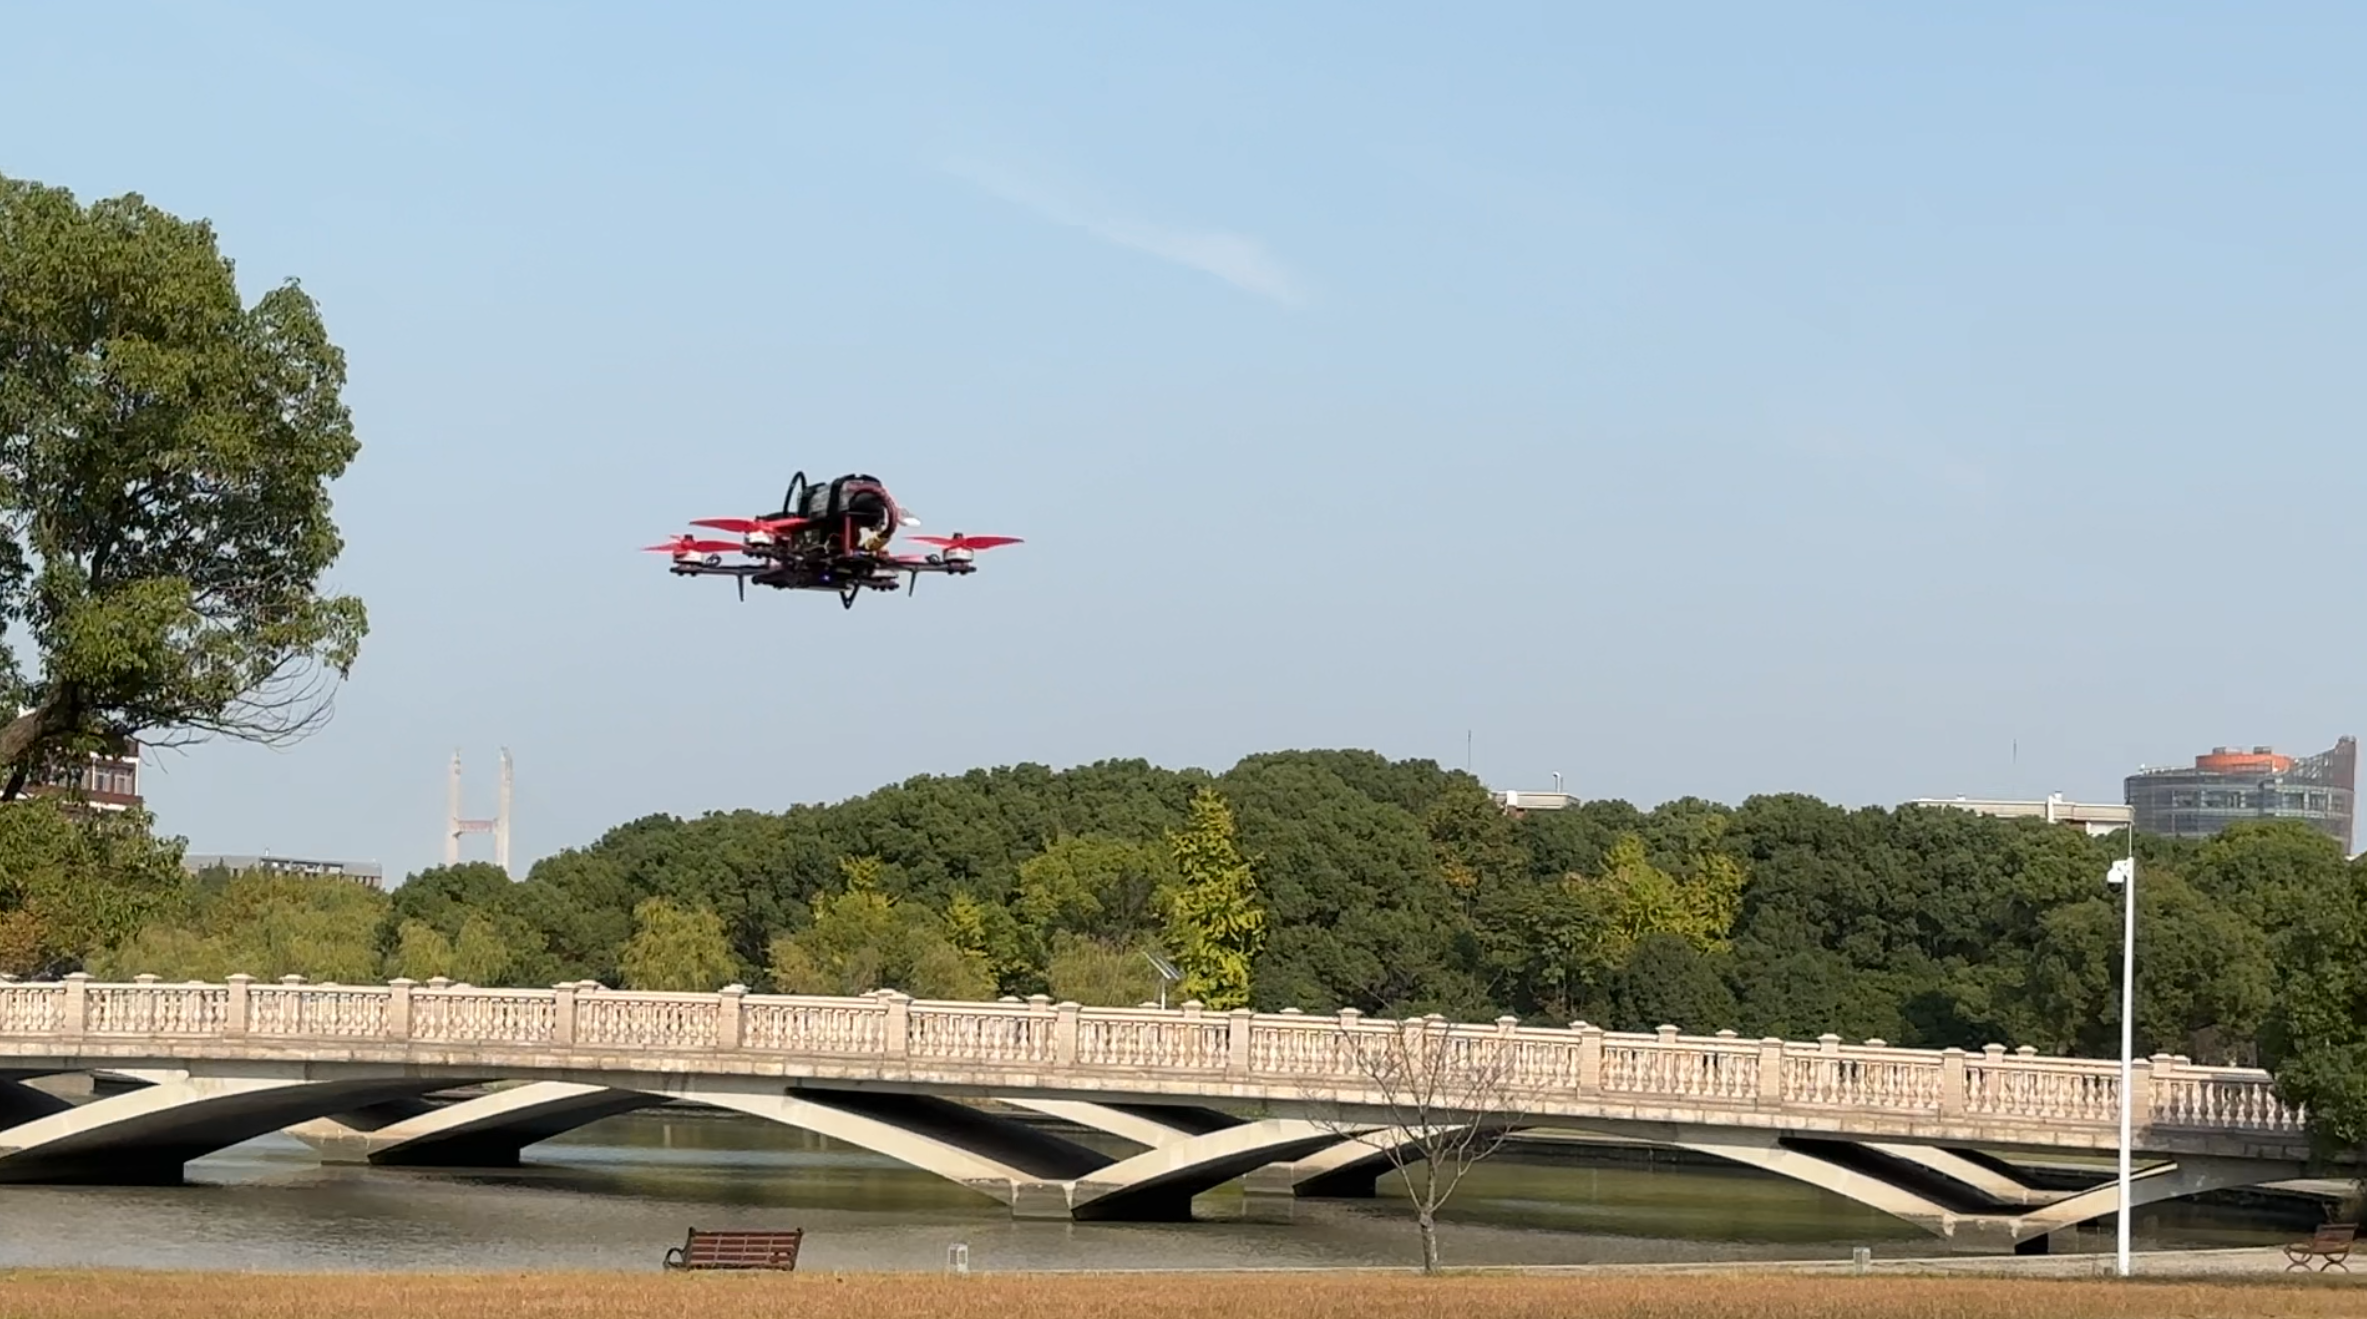
\includegraphics[width=0.95\linewidth]{室外飞行1.png}
  \end{minipage} \hfill
  \begin{minipage}[c]{0.33\textwidth}
    \centering
    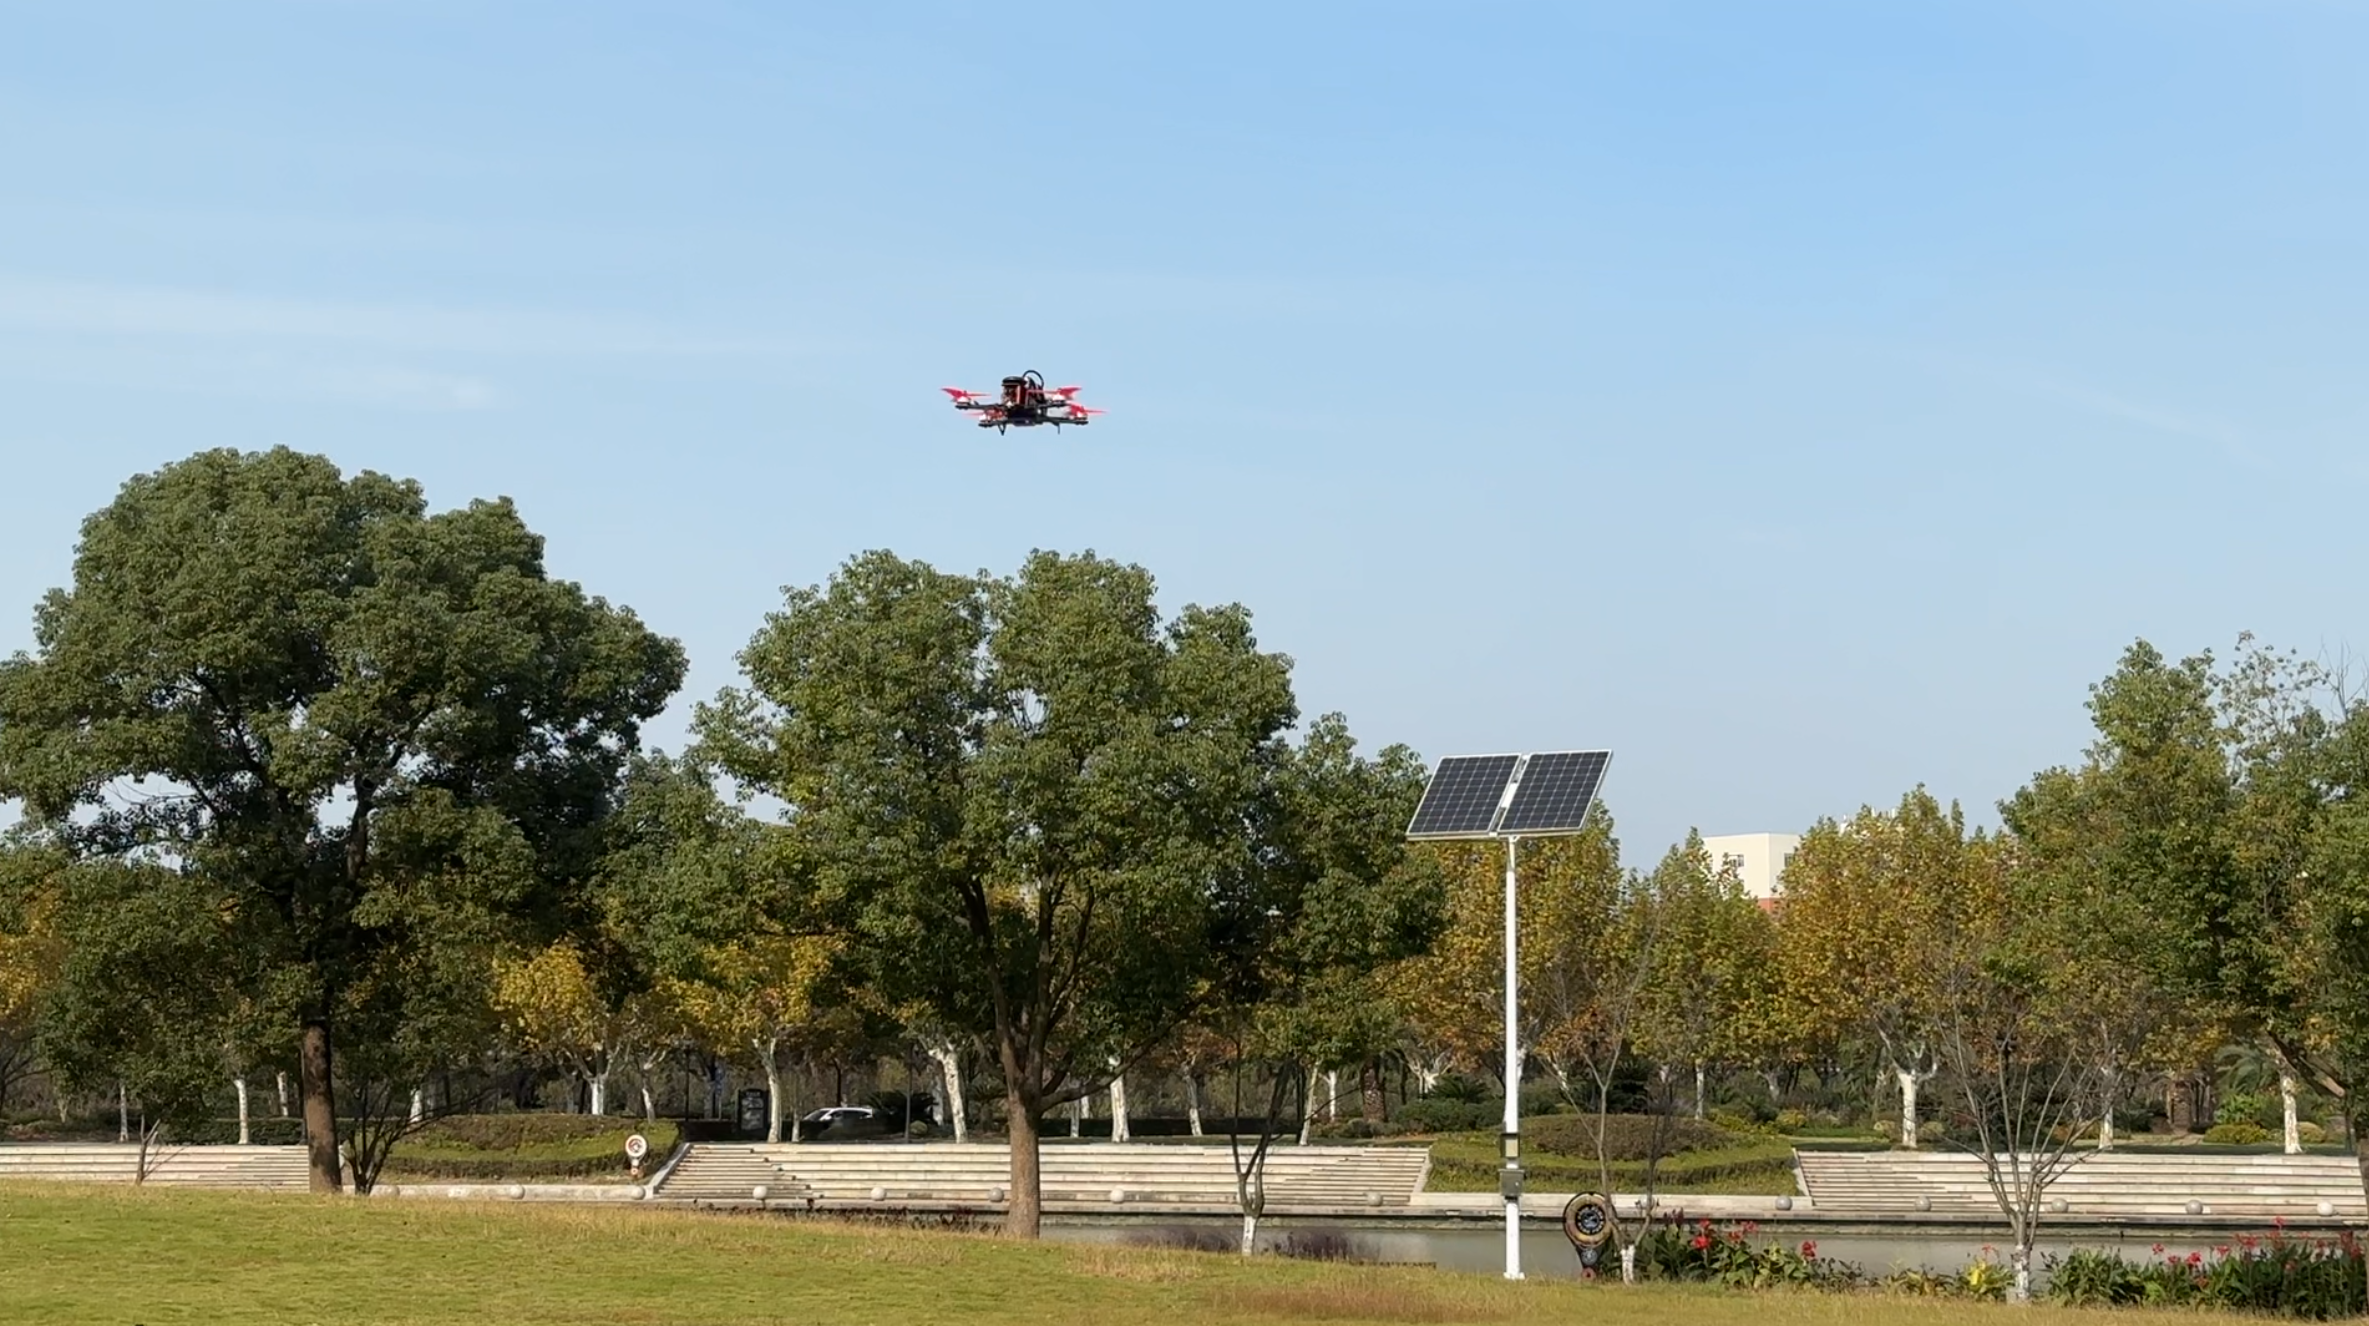
\includegraphics[width=0.95\linewidth]{室外飞行2.png}
  \end{minipage}\hfill
    \begin{minipage}[c]{0.33\textwidth}
      \centering
      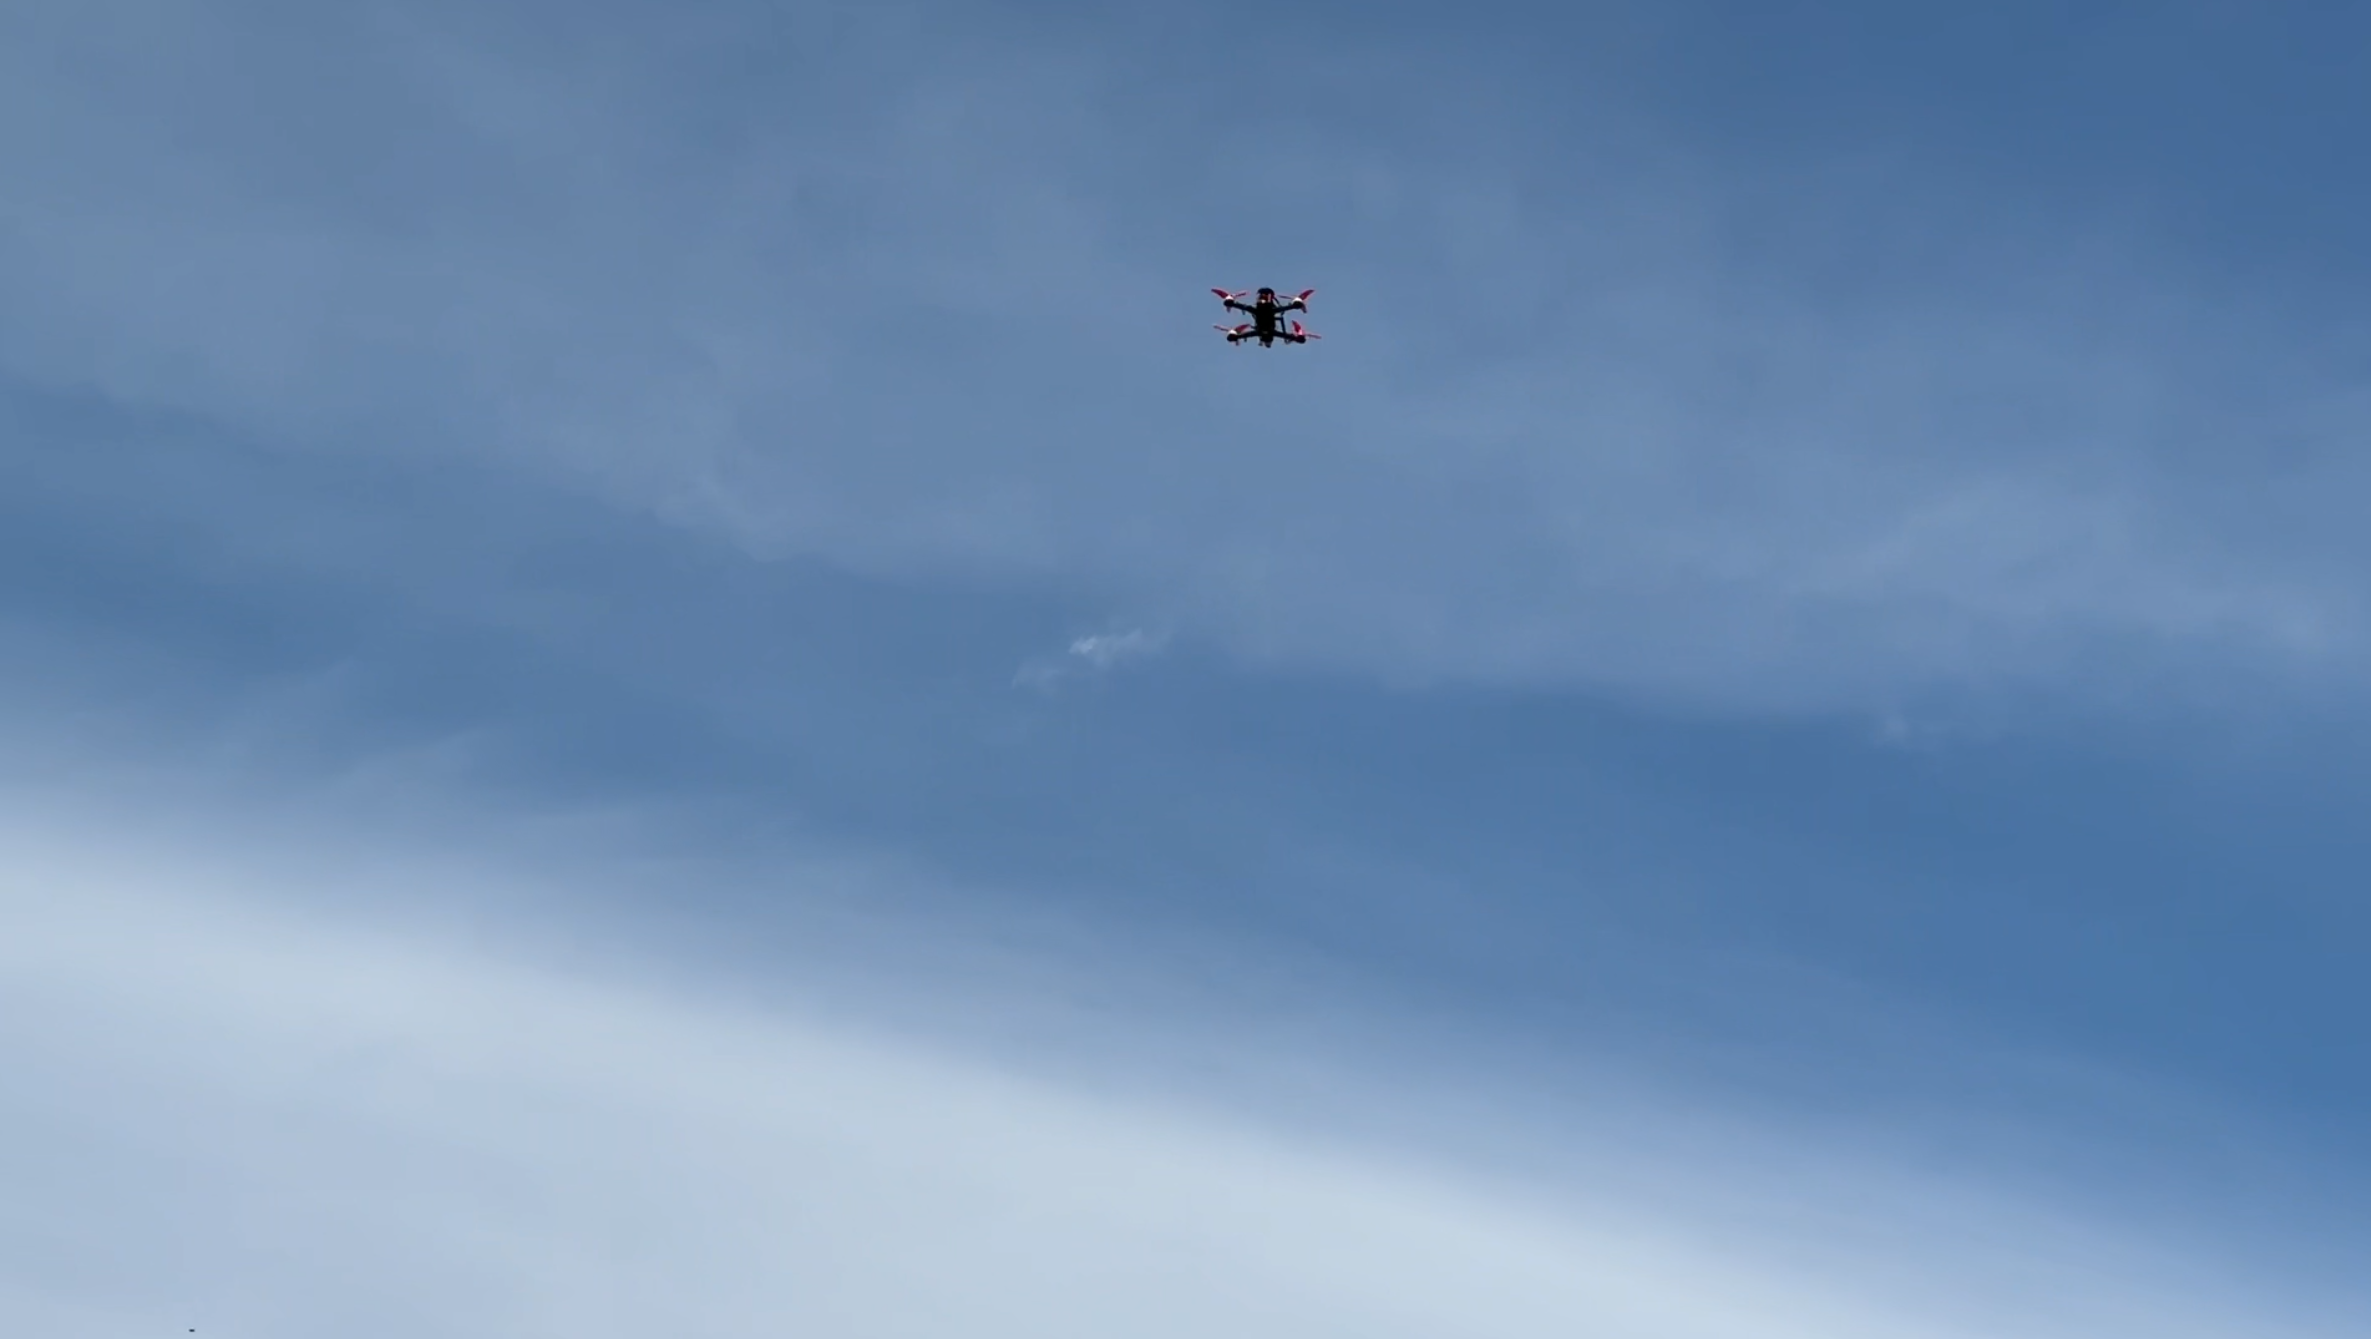
\includegraphics[width=0.95\linewidth]{室外飞行3.png}
  \end{minipage}
  \caption{位置模式下四旋翼室外飞行画面}
  \label{室外飞行}
  \end{figure}

  \section{搭载机载电脑的室内飞行}
室内飞行与室外飞行的主要区别在于位置信息的获得方式。由于室内没有GPS信号,位置信息的获取方式主要有动作捕捉、UWB、自主深度视觉定位和激光雷达等,其中动作捕捉的精度和稳定性最高,并且不用在飞机上增加额外的载荷,所以我们采用了动作捕捉作为本课题的定位方法。

我们采用8台动捕相机吊装在实验场地上方四周,实验场地的尺寸为$5m \times 4.6m \times 2.6m$。在当前配置下,可以达到亚毫米的定位精度和400hz的采样频率\cite{qingtong}。
\begin{figure}[!h]
  \centering
  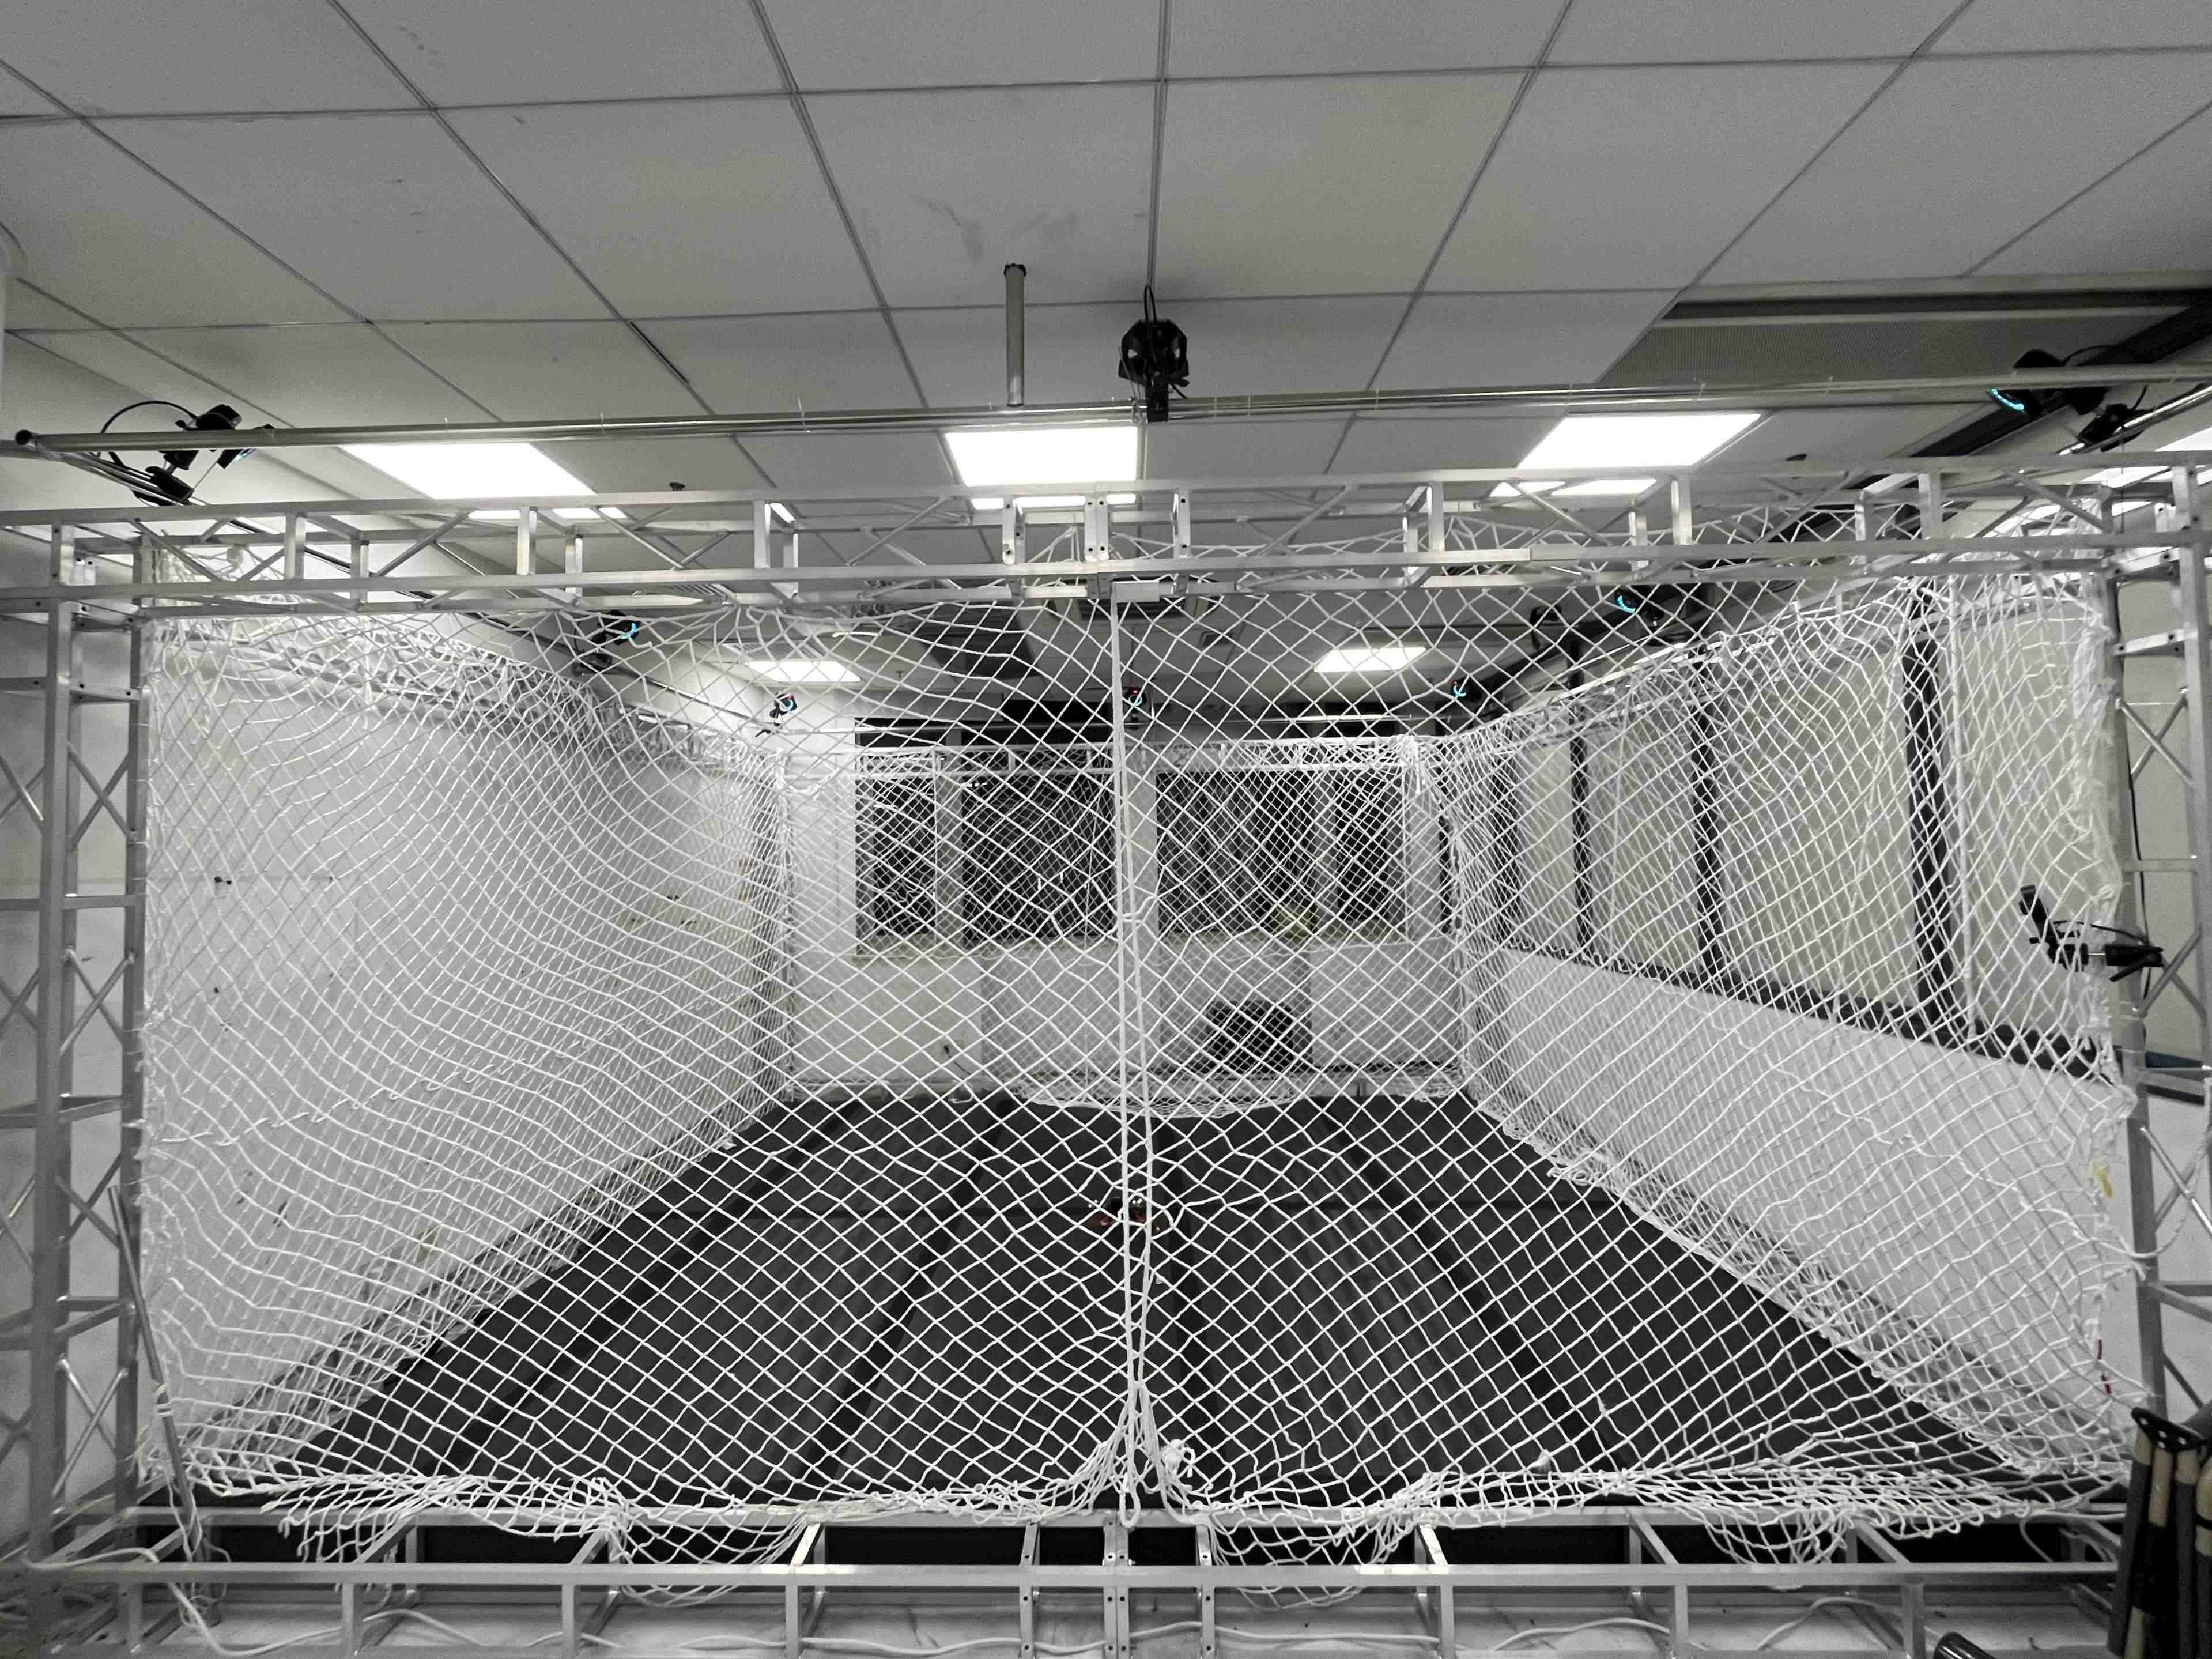
\includegraphics[width=0.6\textwidth]{动捕.jpg}
  \caption{动捕系统以及无人机防撞绳网}
  \label{动捕}
\end{figure}

动捕系统使用红外相机向目标发射红外光,使目标上固连的多个反光小球反射红外光,就能使相机捕捉到,效果如图\ref{反光小球}。

\newpage

\begin{figure}[h]
  \centering
  \begin{minipage}[c]{0.48\textwidth}
    \centering
    \includegraphics[width=0.95\linewidth]{飞机反光球.jpg}
  \end{minipage}\hfill
    \begin{minipage}[c]{0.48\textwidth}
      \centering
      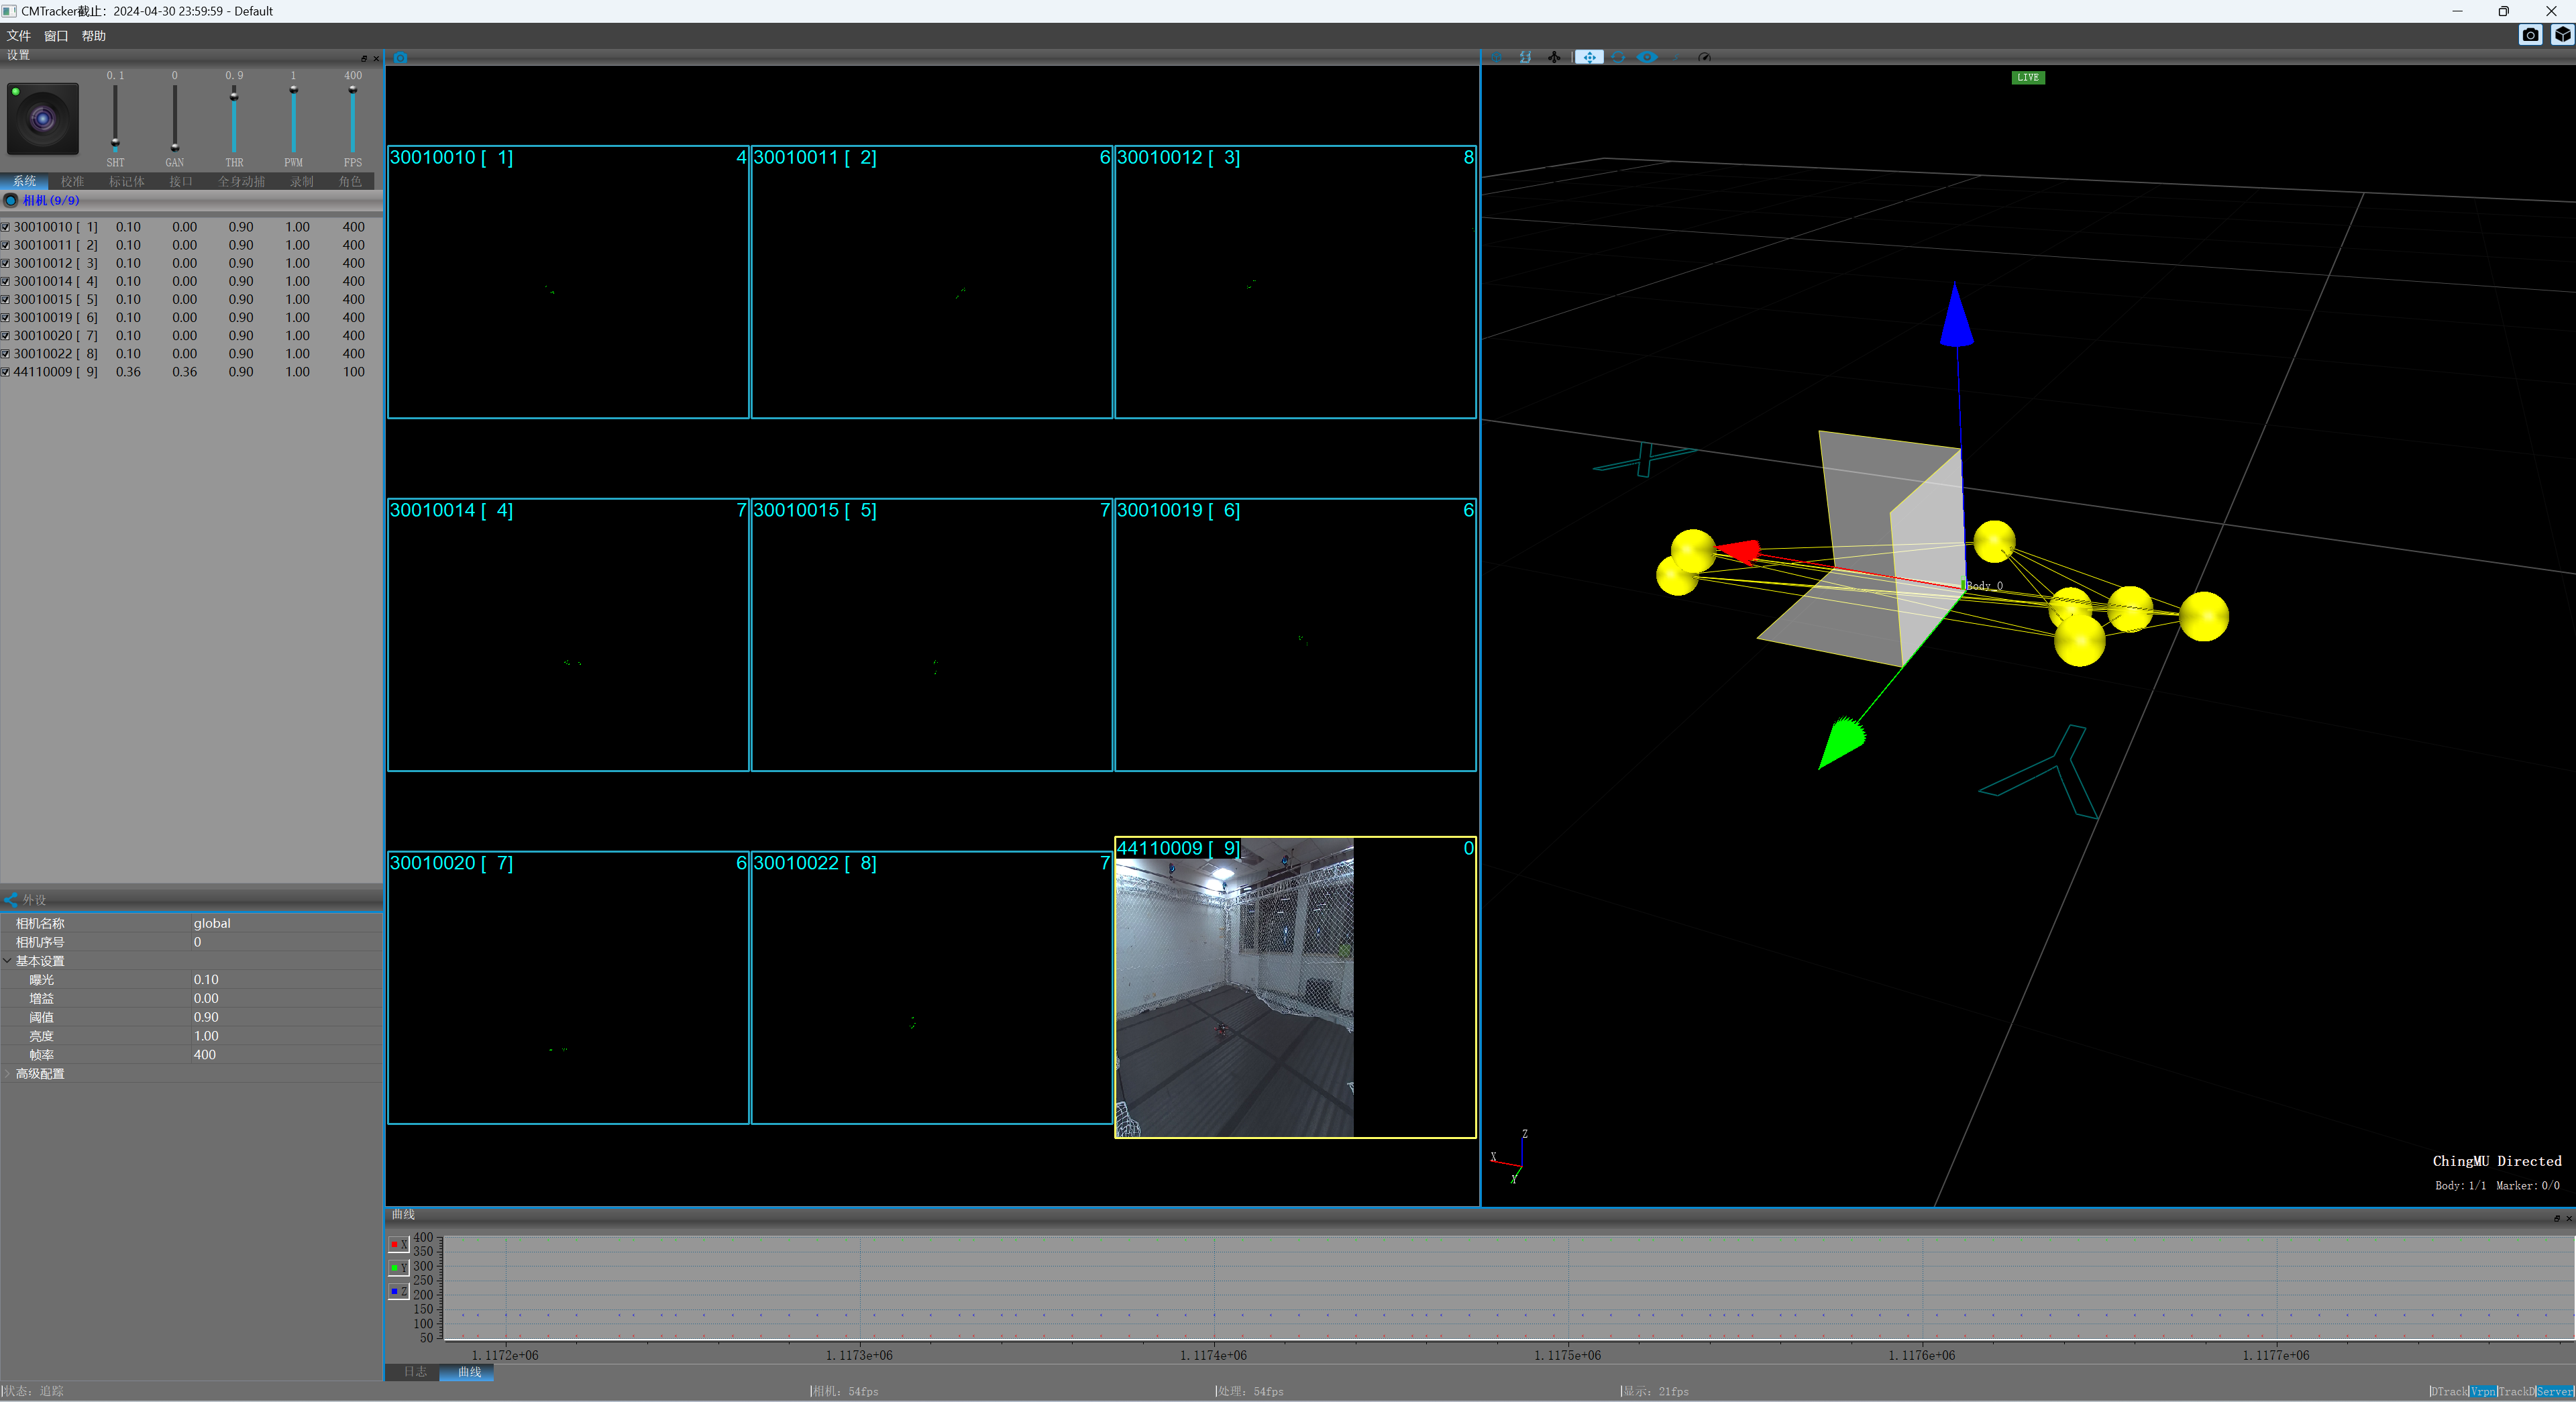
\includegraphics[width=0.95\linewidth]{动捕效果2.png}
  \end{minipage}
  \caption{动作捕捉定位反光小球}
  \label{反光小球}
  \end{figure}


由于相机通过扫场校准已知自身位置,多台相机的二维信息融合在一起就可以解算出目标的位置和姿态。

相机在拍到反光小球后首先在内部做一次图像处理,提取反光点位置,然后通过网线传到动捕服务器上。所有的相机和东部服务器都通过网线连在一台交换机上,形成一个局域网。动捕服务器在汇总了所有信息后解算出目标刚体的位置和姿态,然后以固定的数据报协议在其所在的所有局域网内广播。动捕服务器在用网线连接交换机之外,还和机载电脑连接同一个wifi,也就是说动捕服务器同时处在两个局域网中,而机载电脑也可以通过wifi这个局域网收到位姿广播。

在ros1的架构下,飞控和电脑需要存在有线连接才能通过运行mavros包下的px4.launch,经/dev/ttyACM0端口,将飞控虚拟化为一个ros节点。同时运行vrpn-client-ros包内的sample.launch,接受局域网内的位姿广播。最后运行topic-tools relay命令,将位姿信息转发到mavros节点下的vision-pose/pose话题。运行rqt-graph命令得到消息拓扑图 \ref{rqt}。

\begin{figure}[!h]
  \centering
  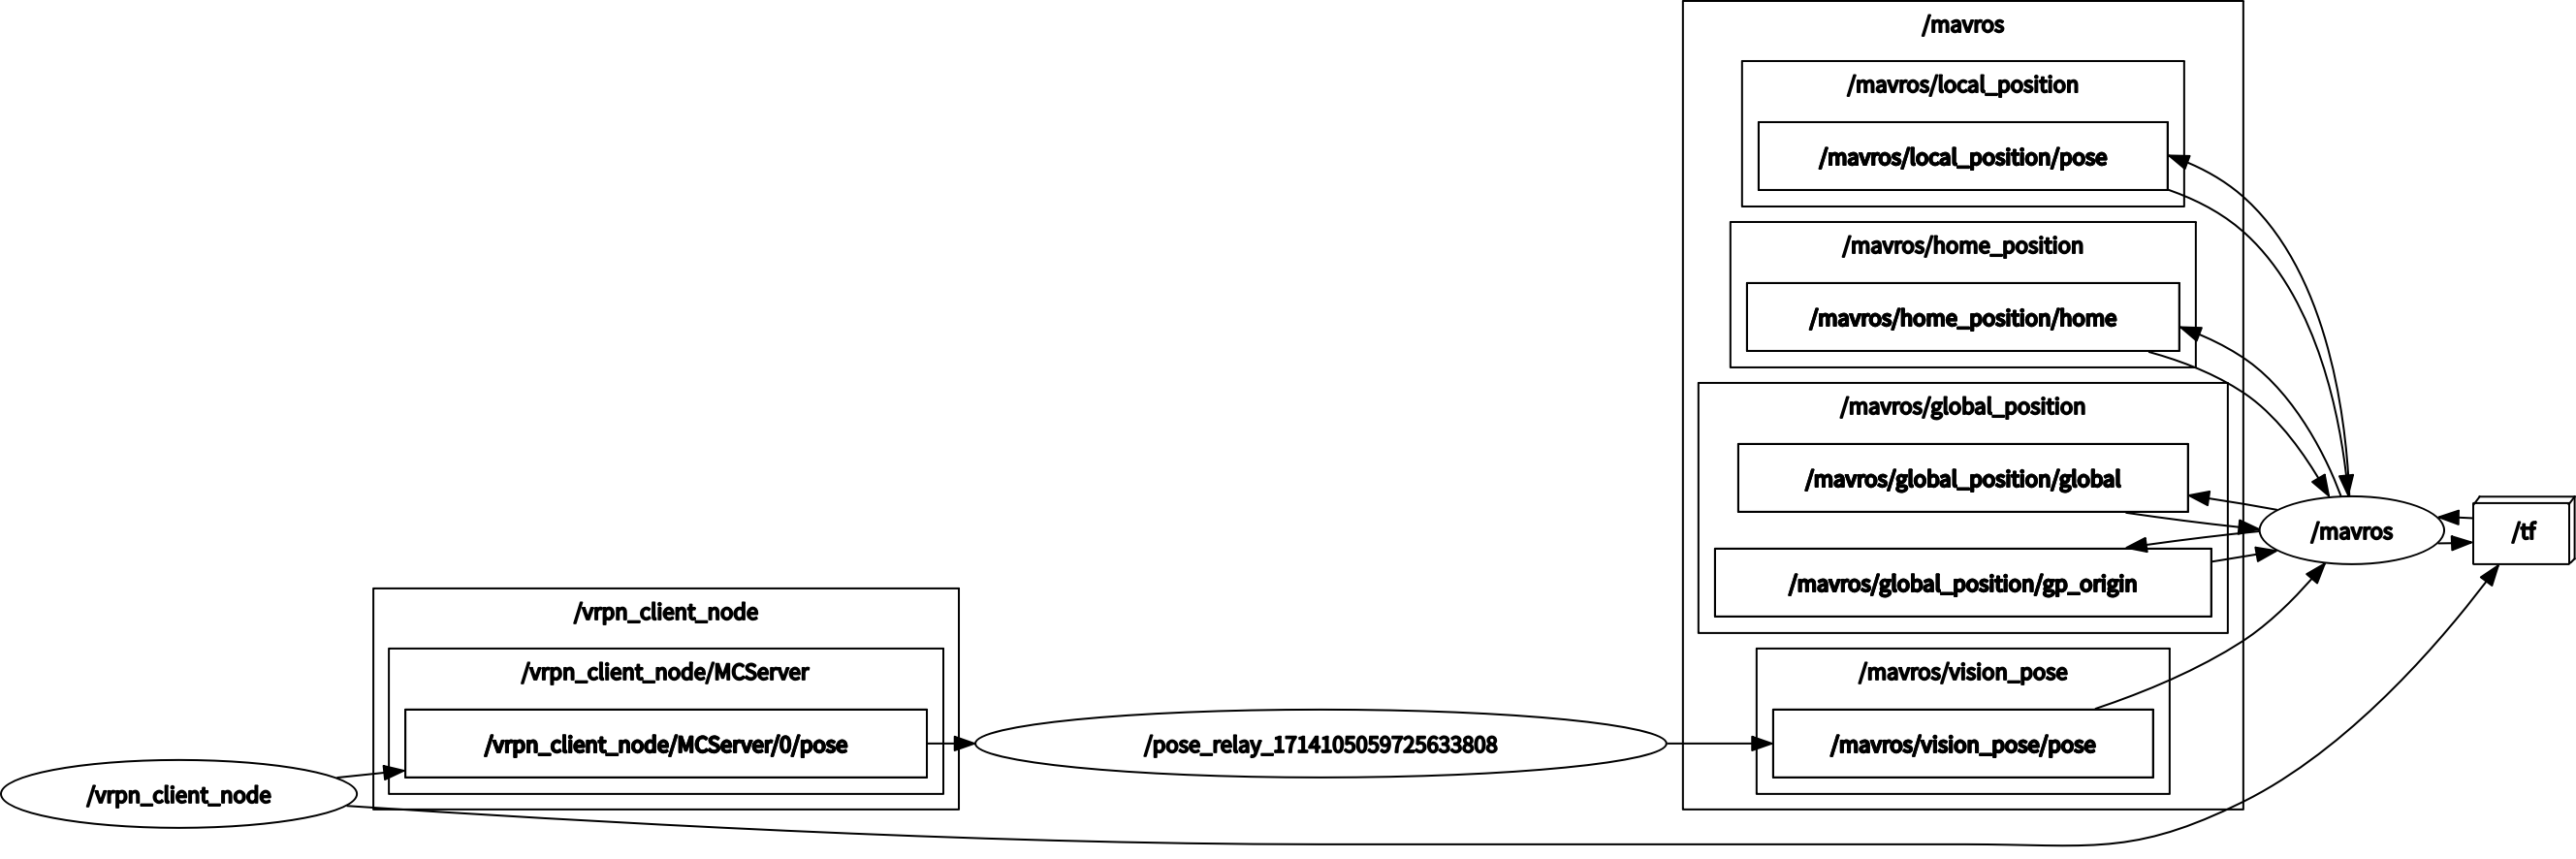
\includegraphics[width=0.9\textwidth]{rqt.png}
  \caption{消息拓扑图}
  \label{rqt}
\end{figure}

以上的这三部分命令可以写到一个bash文件中一键运行,如图 \ref{一键},其中运行px4.launch的参数有gcs-url,这是地面站的ip地址和端口号,mavros会通过wifi与地面站连接,地面站的QGroundControl(QGC)中就能方便地看到无人机目前的状态信息(当然也能通过rviz或rostopic等工具看到),如图 \ref{qgc},也能够发布起飞等指令。

\textbf{local这个坐标系还要再研究一下}

\begin{figure}[!h]
  \centering
  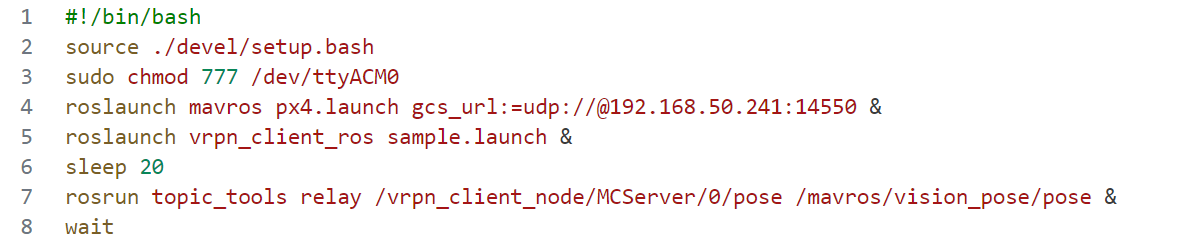
\includegraphics[width=0.8\textwidth]{bash.png}
  \caption{一键启动命令}
  \label{一键}
\end{figure}

\begin{figure}[!h]
  \centering
  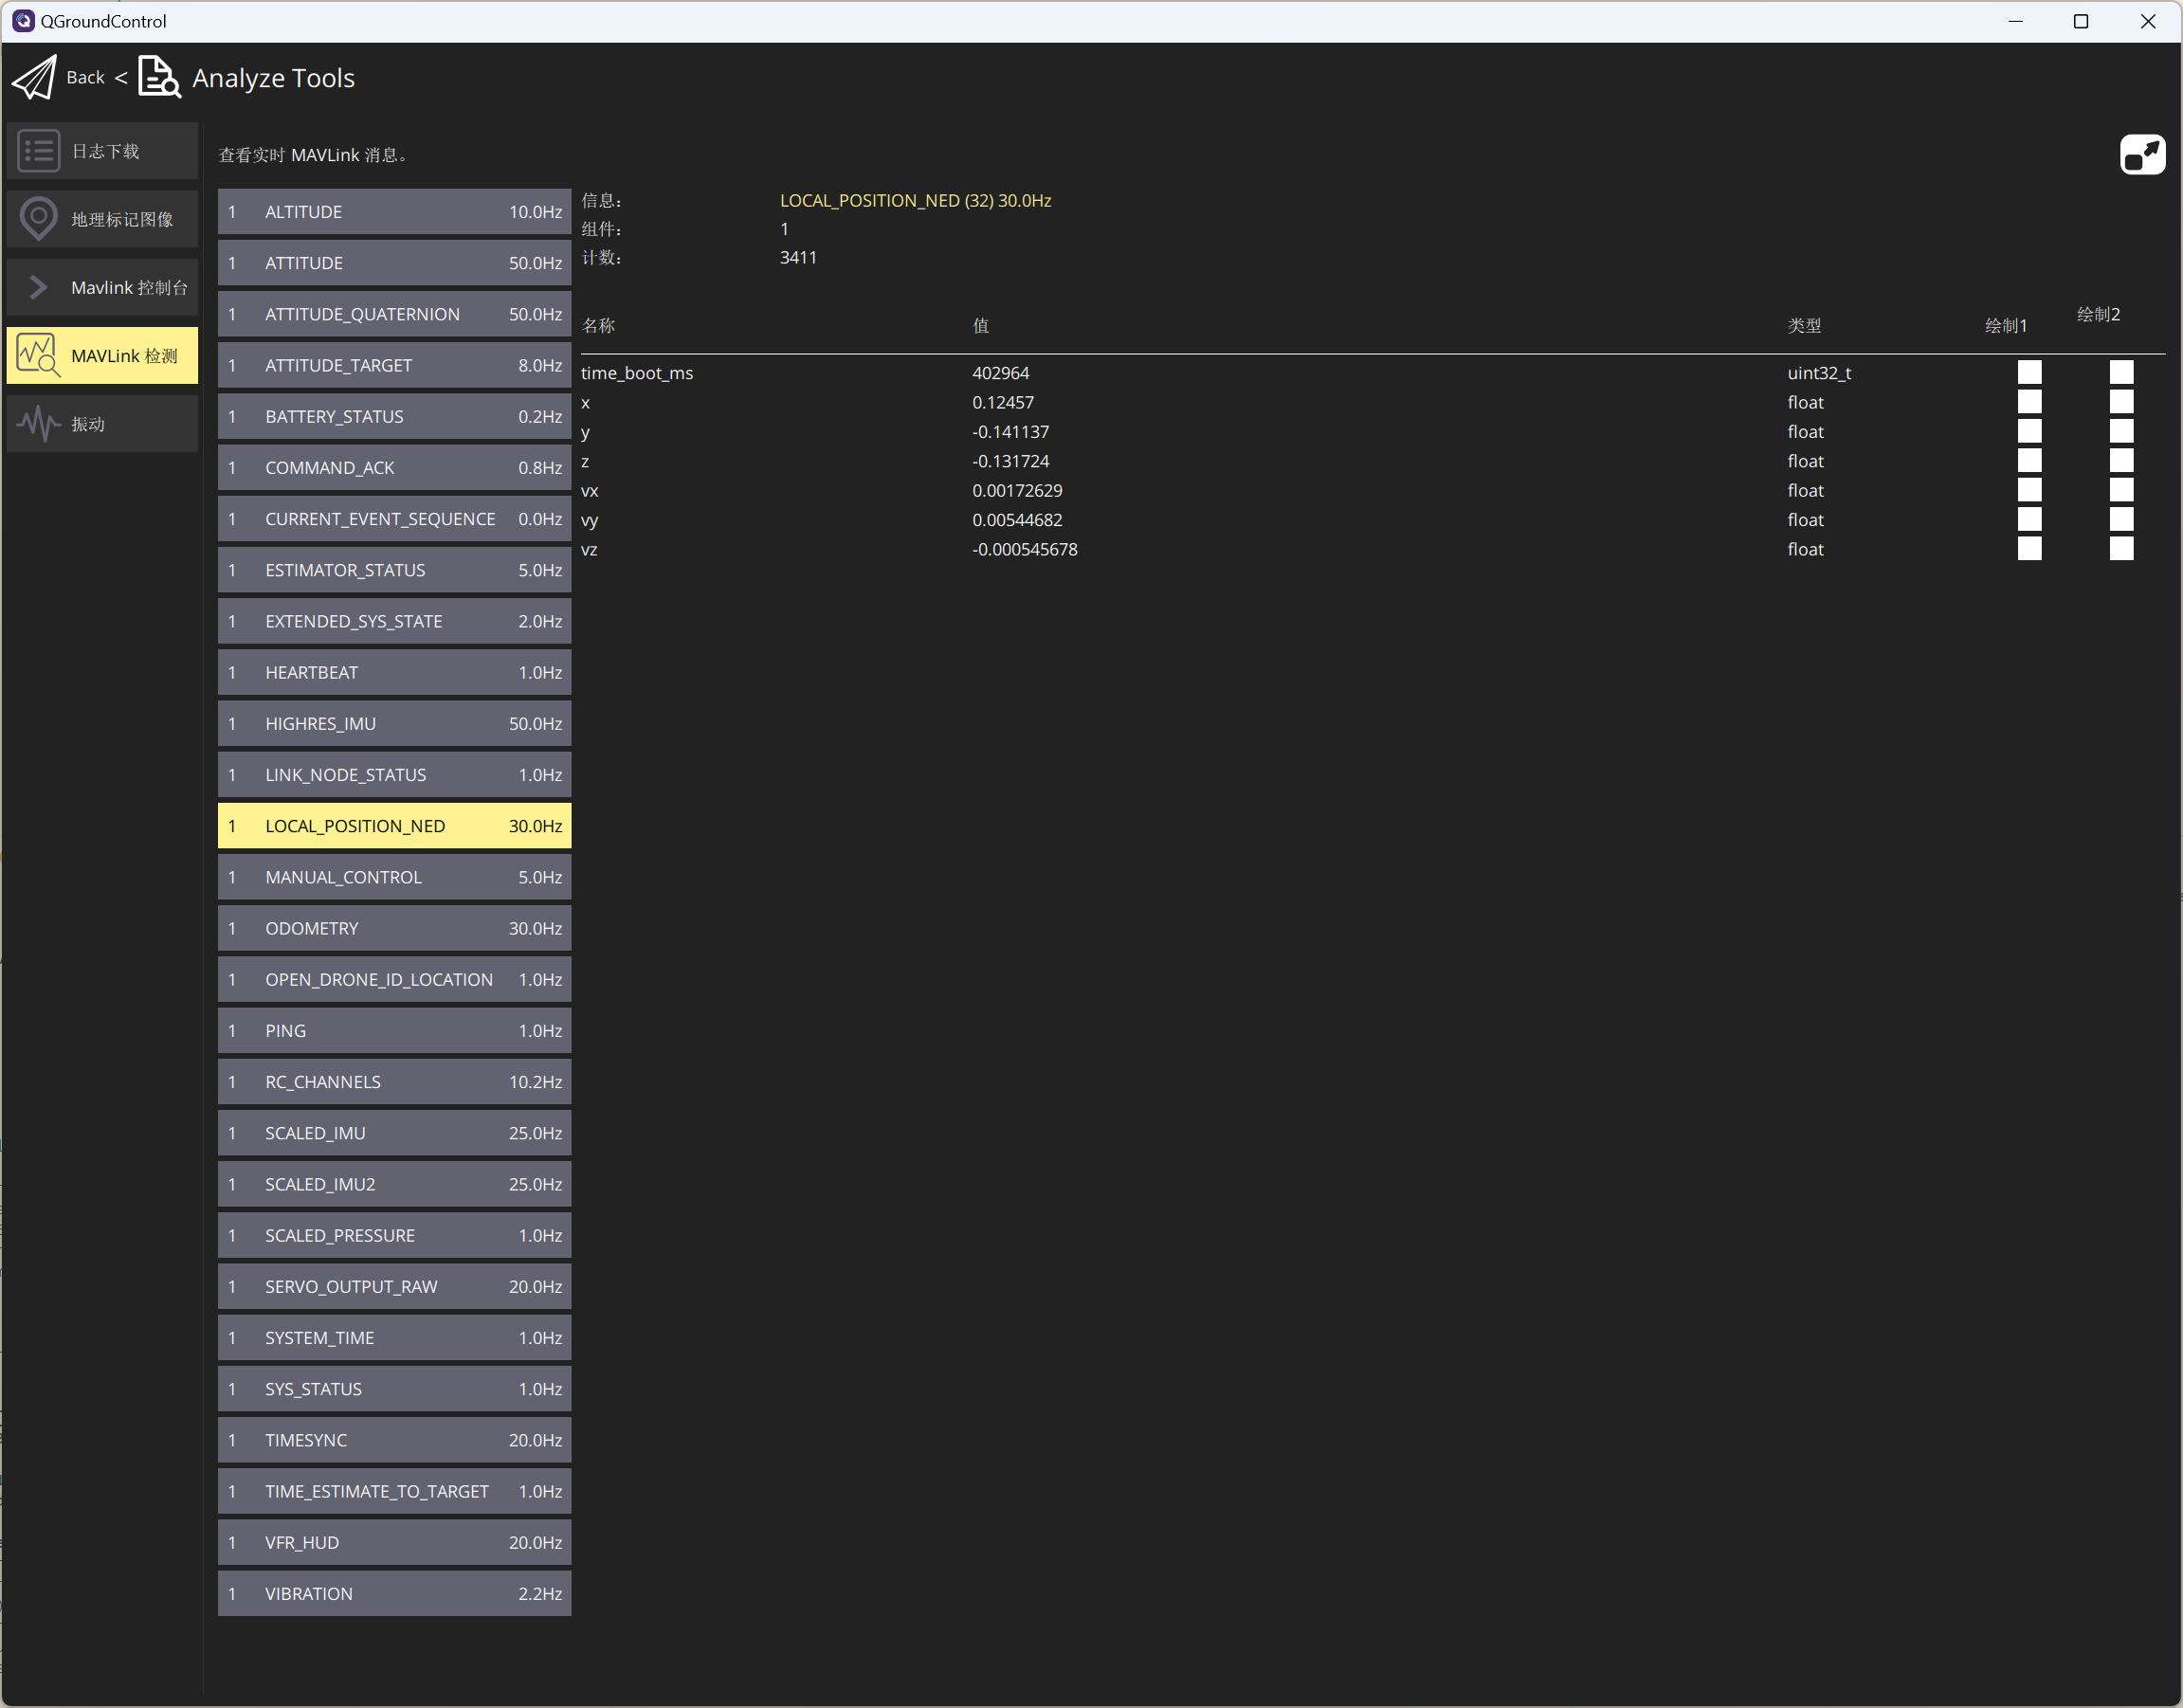
\includegraphics[width=0.5\textwidth]{qgc.png}
  \caption{无人机向QGroundControl传回的信息}
  \label{qgc}
\end{figure}

动捕和飞控内部会各自生成两套坐标系,它们的对齐需要着重考虑。如图 \ref{动捕效果},动捕中无论是全局的坐标还是机身坐标,z轴都是朝上,而如1.2.1节中所说,PX4以及本课题定义的坐标系都是z轴朝下。但由PX4向ros提供的mavros包里,已经考虑了这一点,因为市面上的动捕系统大多都使用z轴朝上的配置。只需要注意飞控上电时的机头指向与动捕中的x轴对齐,z轴朝上,就能对齐两套坐标系\cite{px4moc},而不用关注无人机上电时的位置。PX4内部进行数据融合是会以动捕信息的位置初始值为准,也就是只要方向正确,在场地内的任何地方上电都会按照动捕系统的坐标系配置。

\newpage

\begin{figure}[!h]
  \centering
  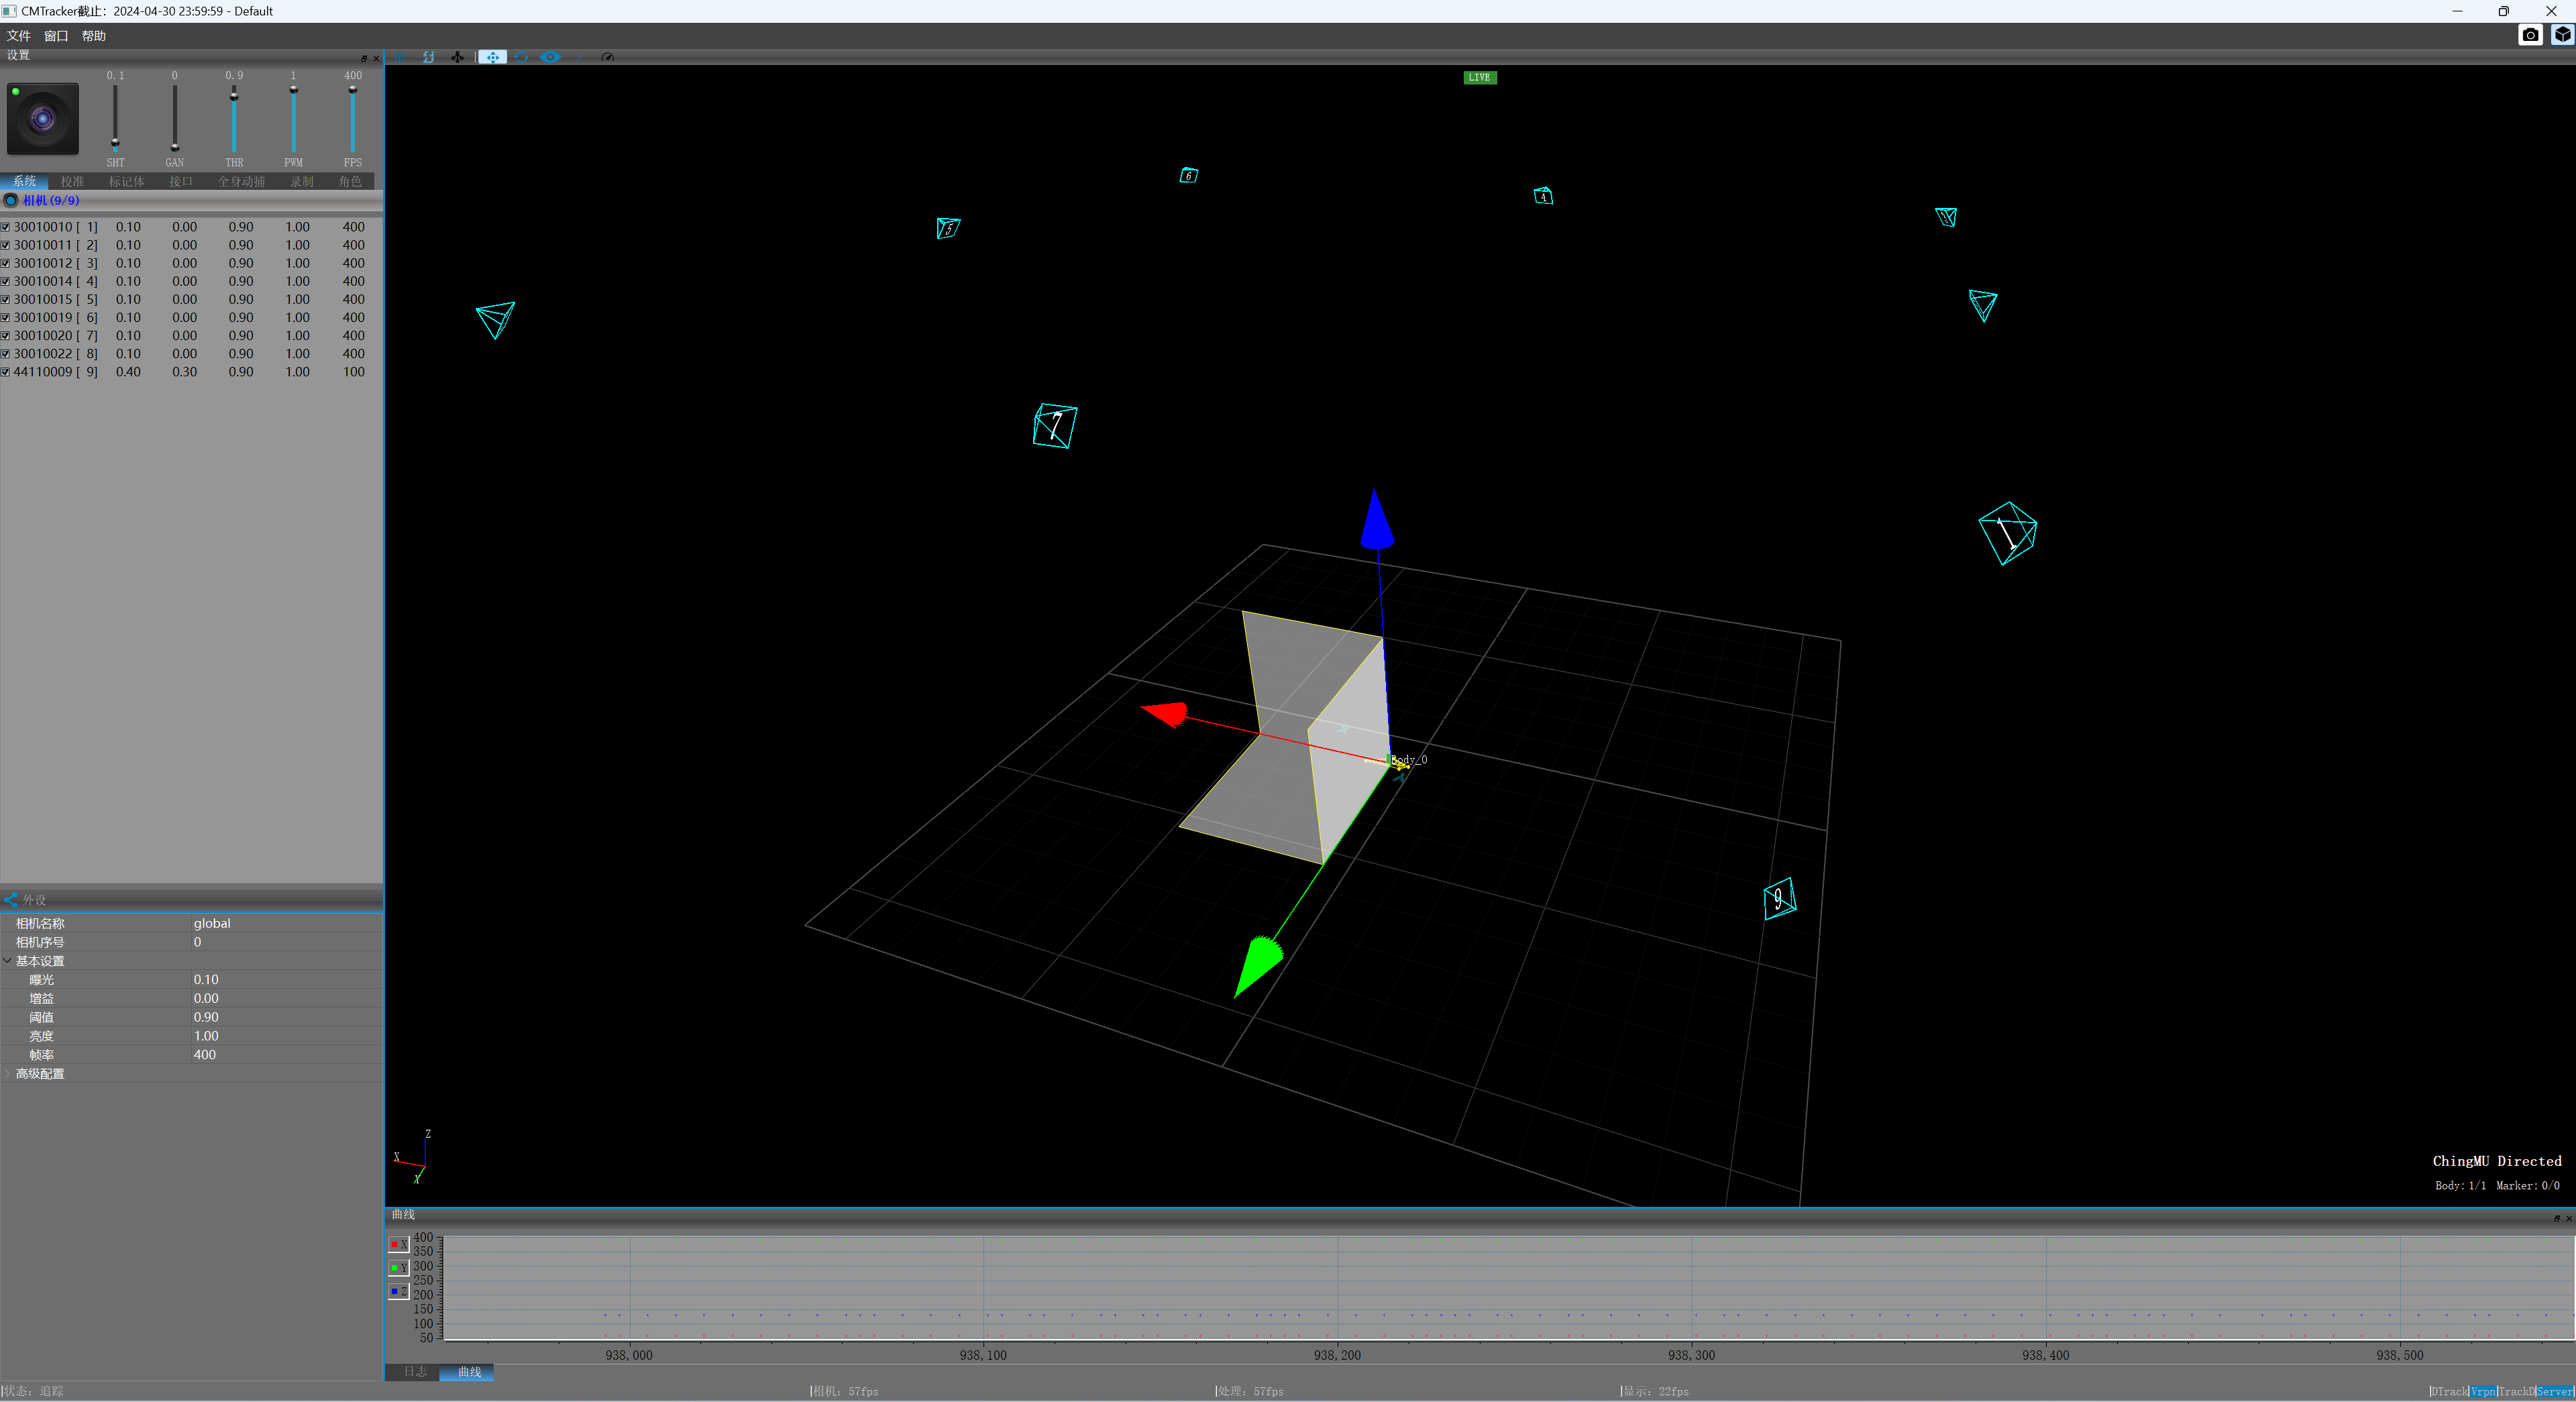
\includegraphics[width=0.6\textwidth]{动捕效果1.png}
  \caption{动捕坐标系设定}
  \label{动捕效果}
\end{figure}

在QGC中查看传回来的位姿信息,多方向移动无人机查看位置变化是否如预期,旋转无人机查看姿态变化是否如预期。需要注意的是QGC中PX4的LOCAL-POSITION-NED、ATTITUDE-QUATERNION、ATTITUDE等话题的坐标系与动捕的坐标系并不相同,如PX4官方文档\cite{px4moc}中示意图所示 \ref{mocpx4}。z轴由朝上改为朝下,x轴与y轴互换,机身坐标系亦是如此(初始时机身坐标系与世界坐标系重合),这也就意味着上电时动捕坐标系下姿态四元数为幺元,而在PX4的坐标系中绕z轴有$90  ^{\circ}$ 的旋转。

\begin{figure}[!h]
  \centering
  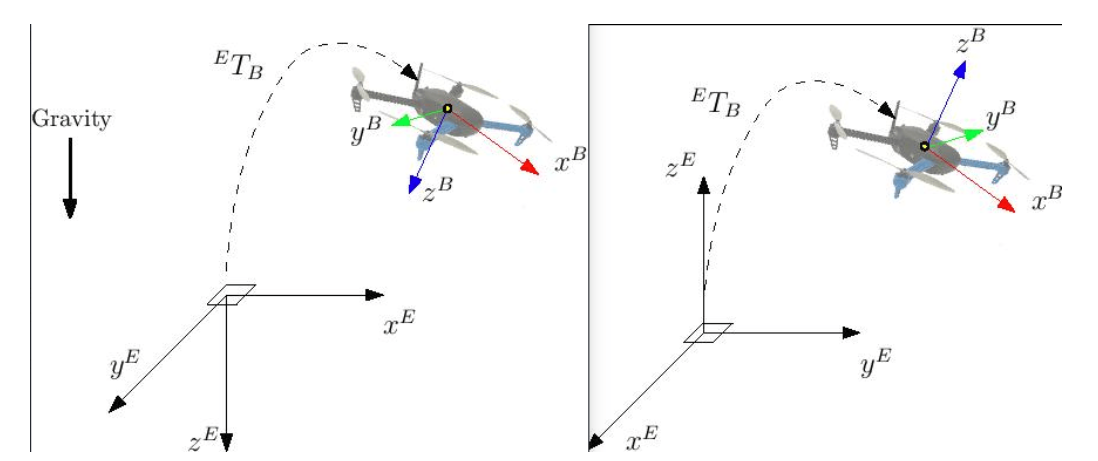
\includegraphics[width=0.7\textwidth]{mocpx4坐标.png}
  \caption{左图为PX4内坐标系,右图为动捕系统坐标系}
  \label{mocpx4}
\end{figure}

\newpage

在上述检查确认无误后,可以选择在QGC中一键起飞,也可以在位置模式下的遥控器上拨动摇杆起飞。飞行的效果如图 \ref{室内飞行} 所示,可以很好地跟踪遥控前后左右和偏航的指令。

\begin{figure}[h]
  \centering
  \begin{minipage}[c]{0.33\textwidth}
    \centering
    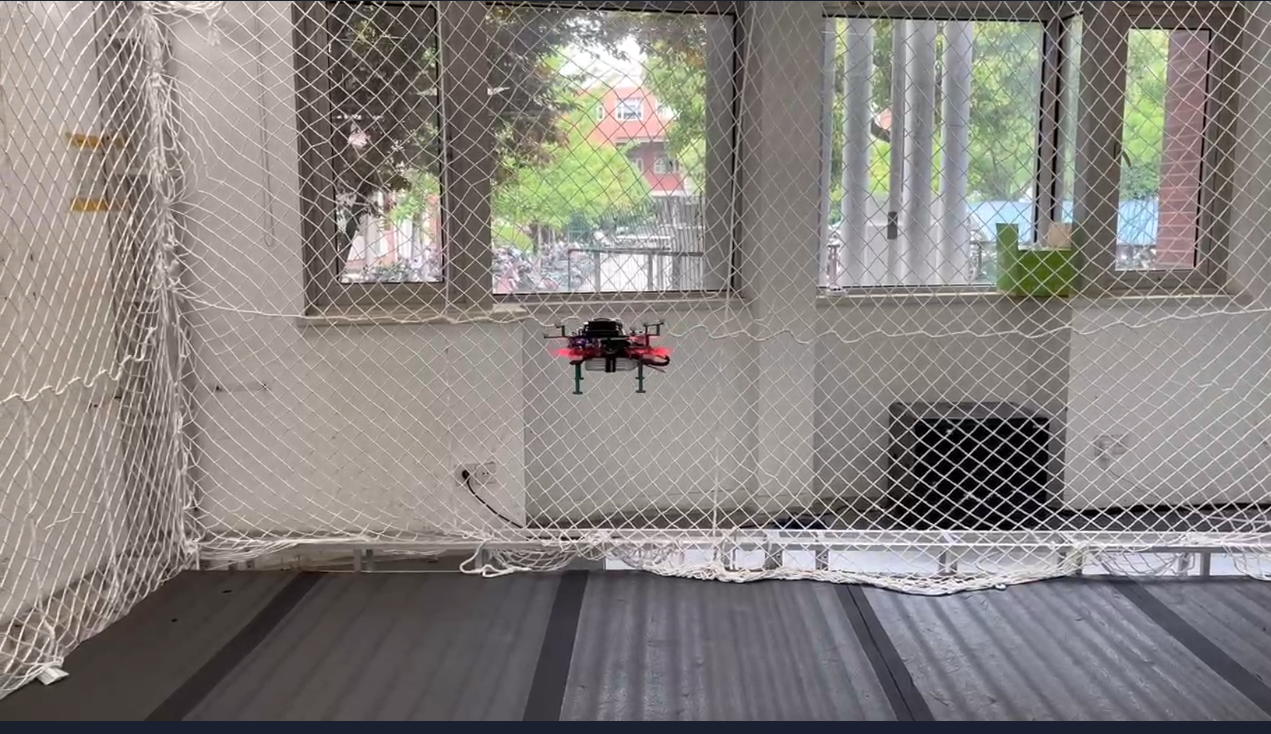
\includegraphics[width=0.95\linewidth]{室内飞行1.png}
  \end{minipage} \hfill
  \begin{minipage}[c]{0.33\textwidth}
    \centering
    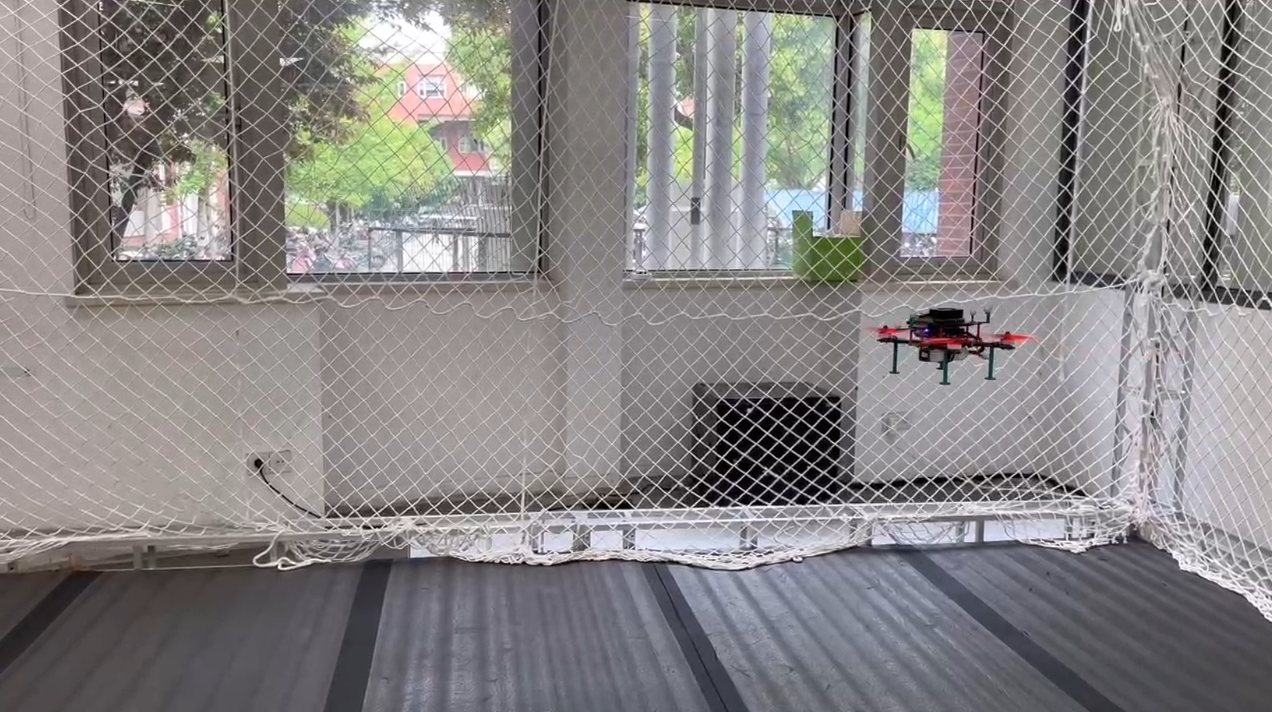
\includegraphics[width=0.95\linewidth]{室内飞行2.png}
  \end{minipage}\hfill
    \begin{minipage}[c]{0.33\textwidth}
      \centering
      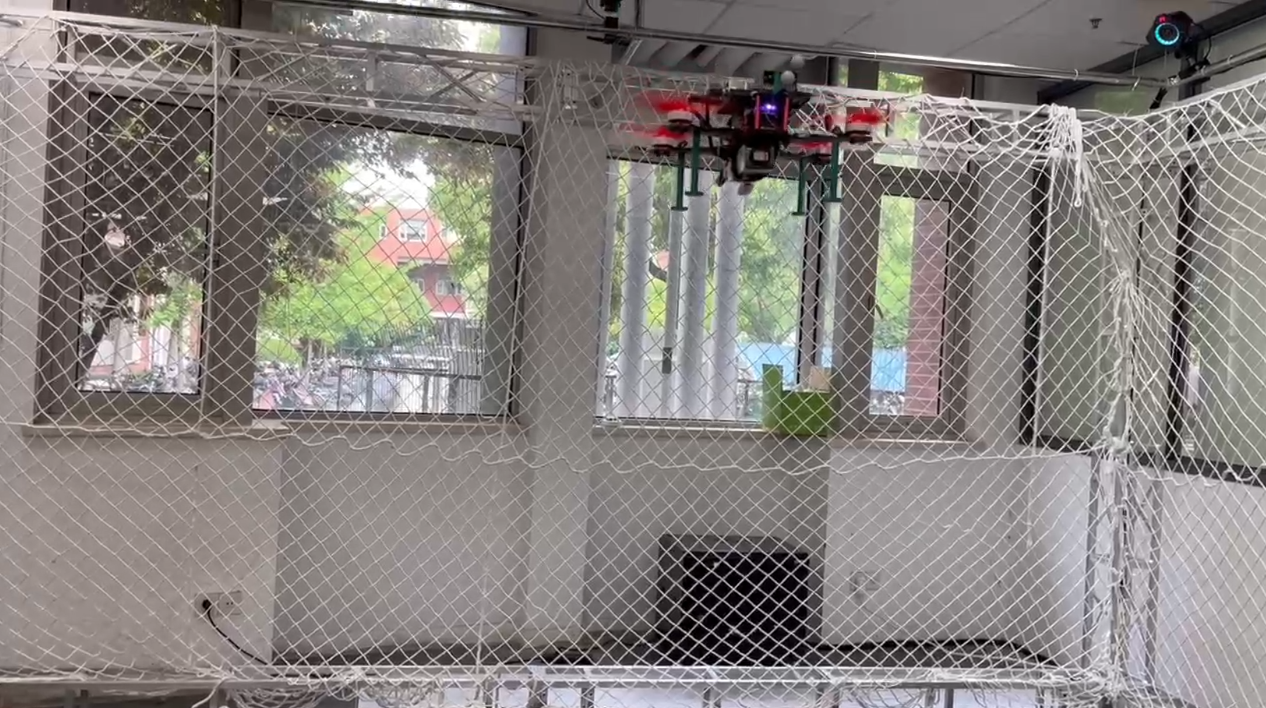
\includegraphics[width=0.95\linewidth]{室内飞行3.png}
  \end{minipage}
  \caption{位置模式下四旋翼室内飞行画面}
  \label{室内飞行}
  \end{figure}

  \section{HOFA固件飞行}

  在仿真实验一章的硬件在环仿真节中得到的飞控固件就可以直接用于实机飞行,但在起飞前需要精确测量无人机的质量和转动惯量参数,以获得更好的飞行效果。

  \textbf{参数测定}

  HOFA算法需要知道无人机的转动惯量矩阵作为先验信息。经过仿真发现,HOFA算法可以容忍较大的转动惯量误差,但如果误差达到十倍的程度,还是会带来破坏性的影响。因此,需要对无人机进行较为精确的转动惯量测定。

  由于四旋翼大体是中心对称结构,因此只考虑转动惯量矩阵对角线上的元素,即中心主转动惯量。主转动惯量可以采用双线摆方法测量\cite{转动惯量}:用两条长度为 $L$ 的细线悬垂待测物体,两细线竖直,间隔距离为$d$,使待测转轴与两线竖直中心线重合,绕转轴轻轻拨动待测物体,使其有 $10 ^\circ$ 以下的转角,记录其摆动五十个周期的时间,重复三次。

  双线摆动能势能之和对时间求导为$0$,得到形如$kx+m\ddot x=0$的方程。易得,转动惯量与周期之间的关系为:

  $$
  J_{ii}=\frac{mgd^2}{16 \pi^2 L} T^2
  $$

  无人机质量$m$由电子天平测得为$0.8771kg$,上海地区重力加速度为$9.794 m/s^2$。

  用双线法分别测量无人机绕x轴,y轴,z轴的主转动惯量,如图\ref{双线法}所示。

  \begin{figure}[h]
    \centering
    \begin{minipage}[c]{0.33\textwidth}
      \centering
      \includegraphics[width=0.95\linewidth, angle=270]{x.jpg}  % 确保角度为0
    \end{minipage}\hfill
    \begin{minipage}[c]{0.33\textwidth}
      \centering
      \includegraphics[width=0.95\linewidth, angle=270]{y.jpg}  % 确保角度为0
    \end{minipage}\hfill
    \begin{minipage}[c]{0.33\textwidth}
      \centering
      \includegraphics[width=0.95\linewidth, angle=270]{z.jpg}  % 确保角度为0
    \end{minipage}
    \caption{双线法测量无人机主转动惯量}
    \label{双线法}
\end{figure}


用以上方法重复测量三次并计算,得到表格\ref{三次}:
  
  \begin{table}
    \centering
    \begin{tabular}{cccccccc}
        \toprule
        组别&d/m  & L/m & 50T/s (1) & 50T/s (2) &50T/s (3) & T/s & $J_{ii} / kg \cdot m^2$\\
        \midrule
        $J_{xx}$ & 0.209 &0.67 & 46.46 & 46.36 & 46.40 &0.9281 &0.0031\\
        $J_{yy}$ & 0.170 &0.66 & 58.40 & 57.96 & 58.37 &1.1649 &0.0032\\
        $J_{zz}$ & 0.271 & 0.65& 42.50 & 42.75 & 42.75 &0.8533 &0.0045\\
        \bottomrule
    \end{tabular}
    \caption{无人机转动惯量矩阵主值测量记录表}
    \label{三次}
\end{table}

最后得到结论$J=\begin{bmatrix}
  0.0031 &0&0\\
  0&0.0032&0\\
  0&0& 0.0045
\end{bmatrix}kg \cdot m^2$,这与matlab仿真阶段的估计差异不大。
%% !TEX root = ../main.tex

\chapter{绪论}
\section{研究背景和意义}

四旋翼无人机由于其高机动性、易于部署、低成本等优势,在近年来得到了越来越多的商业化应用。例如,航拍无人机已经在电影和媒体行业中得到广泛应用(如图\ref{dji}),消费级航拍无人机的市场也空前繁荣,新奇的航拍视角大幅提高了视觉呈现的吸引力和表现力。无人机集群的灯光表演越来越多地出现在大众的视野中,成为节庆典礼的常客(如图\ref{灯光秀})。在农业领域,植保无人机用于监测作物健康和精准施肥灌溉\cite{tokekar2016agricluture},尤其是在地形复杂不利于大型农机作业的地方,显著提高了作物产量和农业资源的使用效率(如图\ref{植保})。在自然灾害发生时,四旋翼无人机在紧急搜救和灾后评估中也显示出巨大的潜力\cite{tomic2012},它们能够快速进入灾区进行空中勘察,为救援队提供实时数据,有助于优化救援计划并减少救援人员的风险(如图\ref{救援})。

\begin{figure}[t]
    \centering
    \begin{minipage}[b]{0.49\linewidth}
        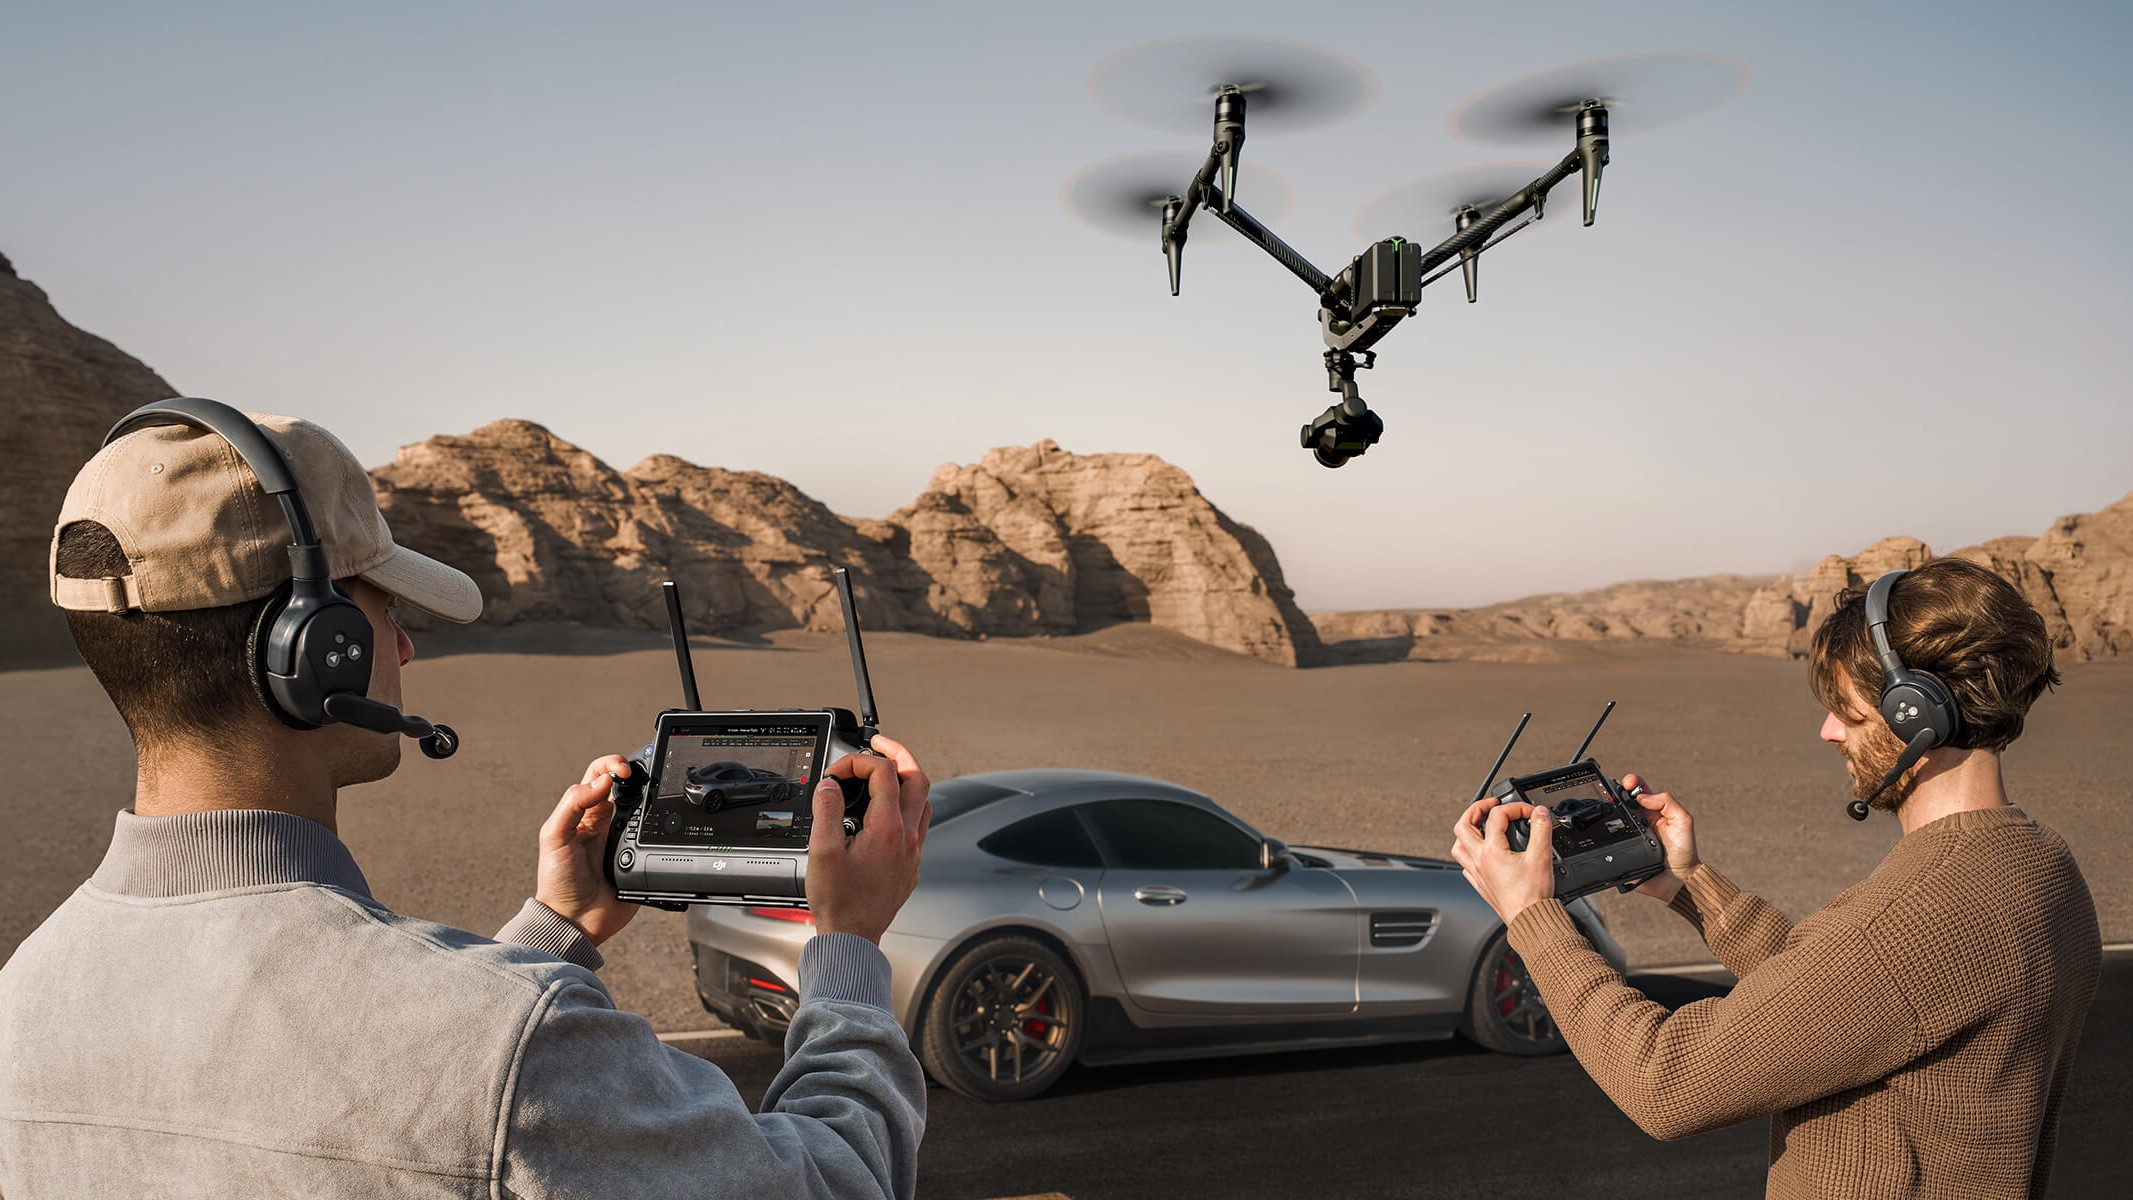
\includegraphics[width=\linewidth]{dji.jpg}
        \caption{航拍无人机拍摄电影\protect\footnotemark[1]}
        \label{dji}
    \end{minipage}
    \hfill % 在图片之间添加一些空间
    \begin{minipage}[b]{0.49\linewidth}
        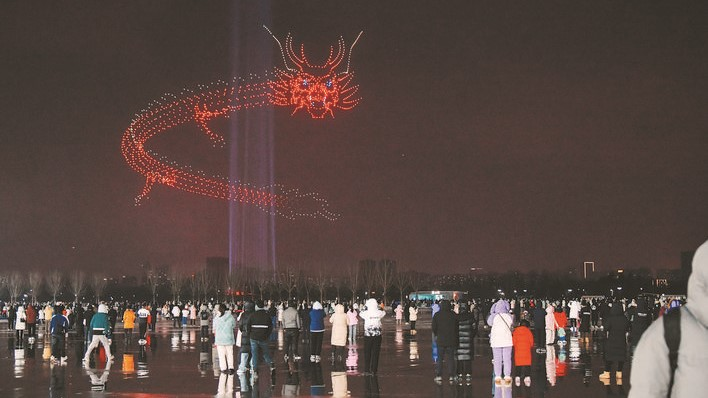
\includegraphics[width=\linewidth]{灯光秀.jpg}
        \caption{无人机集群灯光表演\protect\footnotemark[2]}
        \label{灯光秀}
    \end{minipage}

    \vspace{1cm} % 在行之间添加一些垂直空间

    \begin{minipage}[b]{0.49\linewidth}
        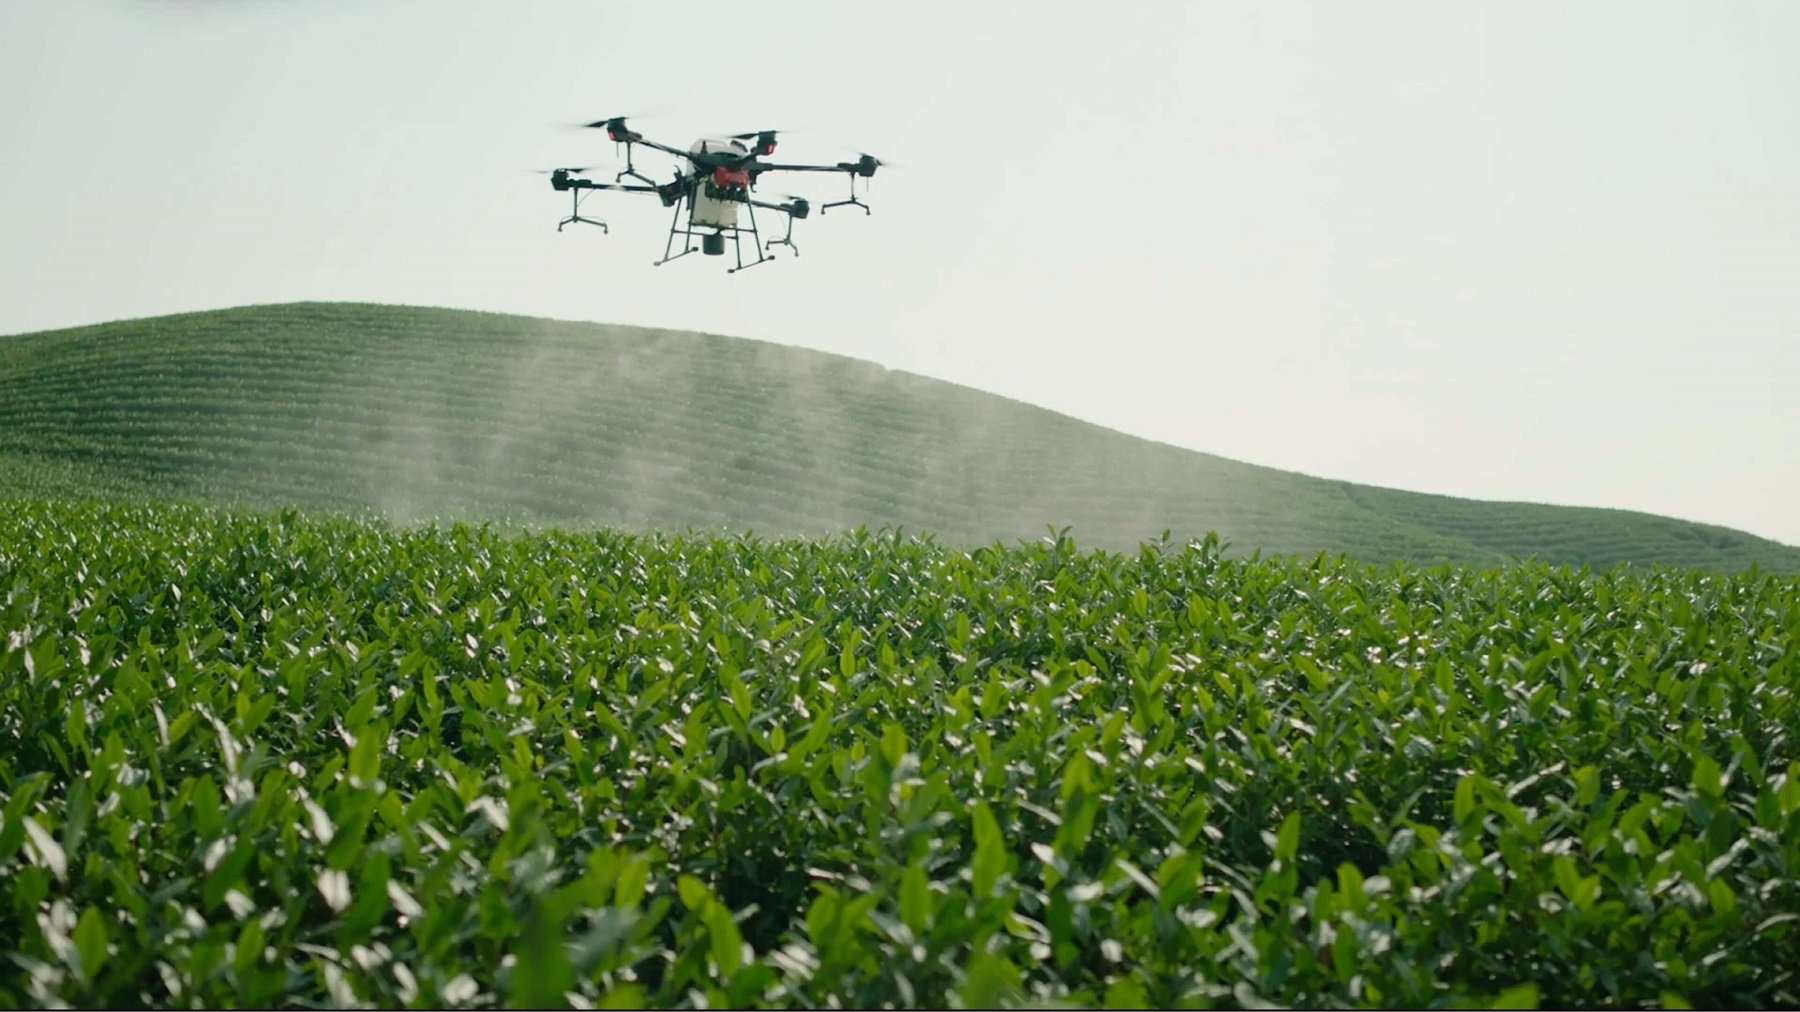
\includegraphics[width=\linewidth]{植保.jpg}
        \caption{植保无人机田间作业\protect\footnotemark[3]}
        \label{植保}
    \end{minipage}
    \hfill
    \begin{minipage}[b]{0.49\linewidth}
        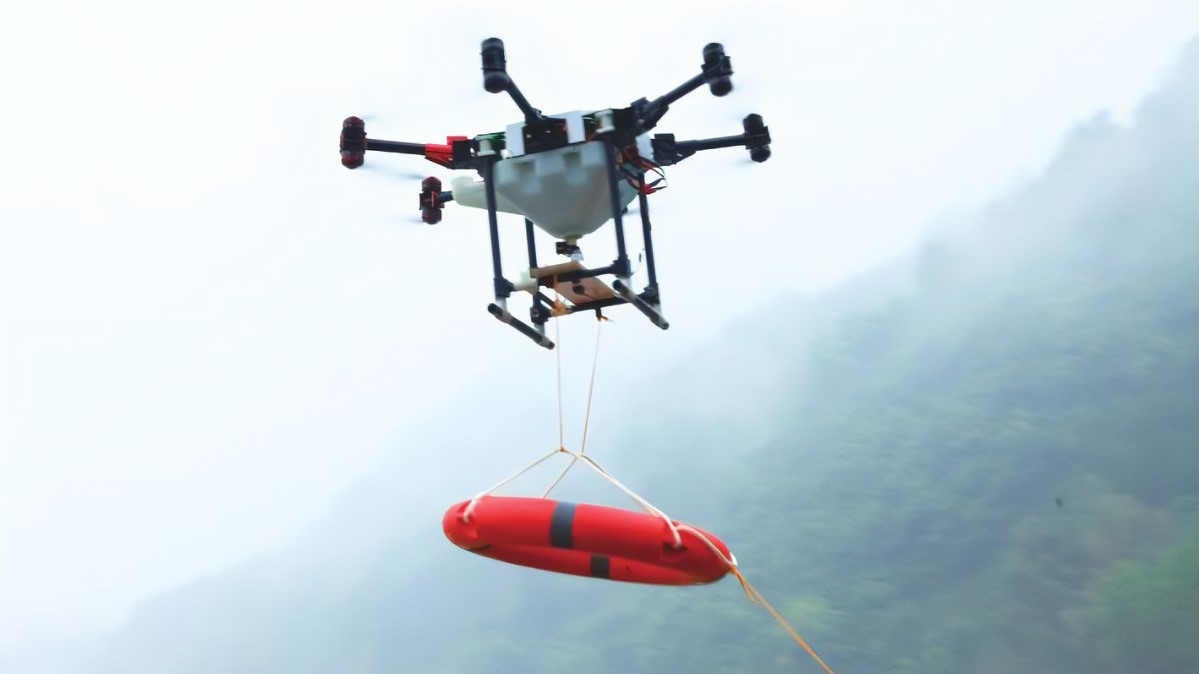
\includegraphics[width=\linewidth]{搜救.jpg}
        \caption{救援无人机水面营救\protect\footnotemark[4]}
        \label{救援}
    \end{minipage}
\end{figure}

尽管四旋翼无人机在许多领域都已经有了落地应用,但它们的飞行控制仍然有进一步完善的空间。飞行动力学的高度非线性、大角度机动时的脆弱稳定性以及传感器对环境噪声的敏感性等仍然是无人机飞行控制要面临的技术难题。这些技术难题的存在,限制了四旋翼无人机在更多高风险或复杂环境中的应用。因此,深入研究和优化四旋翼无人机的飞行控制技术,不仅能够推动无人机技术的进一步商业化,还有助于拓宽其在社会服务和经济活动中的应用范围,如更复杂的城市空中交通管理和多无人机协同作业等新兴领域。

综上所述,四旋翼无人机的研究不仅具有重要的技术意义,更在社会经济和安全等多个层面发挥着越来越重要的作用。因此,本研究旨在通过对四旋翼无人机飞行控制的深入分析和改进,解决现有的技术难题,为其更广泛的应用奠定坚实的基础。

\section{四旋翼飞行控制的研究现状}
四旋翼无人机出于上述的种种优势和应用潜力,近年来得到了广泛研究\cite{survey}。四旋翼具有高度机动性的优势,同时也有欠驱动、载荷算力有限和高控制频率的限制。这使得四旋翼成为验证先进控制理论的理想测试平台\cite{La2018}。
\footnotetext[1]{图片来源:\url{https://www.dji.com/cn/inspire-3?site=brandsite&from=landing_page}}
\footnotetext[2]{图片来源:\url{https://www.scnjnews.com/content/2023-06/25/content_6509732.html}}
\footnotetext[3]{图片来源:\url{https://news.mydrivers.com/1/655/655677.htm}}
\footnotetext[4]{图片来源:\url{https://uav.huanqiu.com/article/9CaKrnK3V5e}}


随着近年来计算机处理能力的增强以及传感器的发展,关于无人机控制的研究快速发展。
2004年,Bouabdallah将角速度近似等于欧拉角的导数,得到简化后的四旋翼动力学方程,在此基础上他分步解决姿态跟踪和高度跟踪的问题。他使用了简单的闭环反馈作为控制器进行仿真和实机实验,证实了其控制姿态角的能力\cite{boua2007}。但这一阶段的工作还比较粗糙,在姿态角较大时将角速度近似等于欧拉角会带来很大的偏差。其控制器几乎只是依赖调参,抗扰动能力较差,并且也只做到了悬停的高度控制。2005年,Bouabdallah和Siegwart进一步提出了反步法和滑模控制两种非线性的方法\cite{boua2005},实现了四旋翼的位置控制并增强了抗扰动能力。虽然还是根据近似后的动力学模型,但反步法能够在较高扰动的情况下做到对方向角的控制。而滑模控制由于开关特性引入了高频低振幅的振动,引发严重的传感器漂移,导致控制效果并不理想。2007年他们在此基础上提出了改进的积分反步法\cite{bouabdallah2007full},也就是将角速度期望设为角度误差的PID控制器输出,达成了更好的角度控制。但受限于电机的响应速度,抖动仍然存在。积分反步法也应用在了位置控制的环节,做到了自动起降、悬停和避障。这一系列的工作在当年是开创性的,但由于传感器精度和频率、执行器性能的限制,其表现在今天看来还是较为不足。

以上的工作对期望位姿的解算实质上欠缺物理意义。而T. Lee等人于2010年提出了针对四旋翼复杂机动的SE(3)非线性控制\cite{Lee2010},在没有对动力学近似的情况下,对这个问题做了物理上合理的解答。由于四旋翼的合推力总是垂直于机身平面,所以将位置环通过前馈和反馈控制算出的期望推力方向作为期望的z轴指向,再由用户输入的期望机头朝向投影得到期望的x轴朝向,由此构建起了完整的期望姿态。为了设计姿态的控制方法,他们根据罗德里格斯公式,由旋转矩阵的迹得到等效绕轴旋转的角度,并将其作为误差。随后从李雅普诺夫稳定性出发设计姿态控制律,在一系列极为巧妙的数学推导后得到了指数收敛的控制器。该控制方法能够跟踪输入的三维位置和一维的机头朝向,几乎拥有全局指数收敛性,通过仿真证实了其良好的控制效果。

2010年,后来风靡全球的开源飞控PX4发布\cite{brescianini2013nonlinear},它将四旋翼的控制分为位置、速度、姿态、角速度四个环,每个环都只采用了简单的PID控制,便于普通用户调试且能很好地适配不同参数的航模。在最重要的姿态环,它用四元数表示下的旋转作差得到期望的角速度。由于传感器技术的发展,IMU和陀螺仪的更新频率大幅增加,使得高频率的内环控制成为可能。

针对无人机模型参数不确定和存在测量噪声的情况,A. C. Satici提出的鲁棒最优控制器在$L_1$最优意义上使误差幅度呈指数下降,最小化系统相对于扰动的$L_\infty$增益\cite{satici2013robust}。
由于不同风况对无人机飞行的影响难以建模,所以Michael O'Connell等人提出了通过深度学习结合预训练的Neural-Fly\cite{o2022neural},以实现快速在线适应。Neural-Fly 实现了精确的飞行控制,跟踪误差比最先进的非线性控制器和自适应控制器还要小得多。除了强大的经验性能之外,Neural-Fly 的指数稳定性还带来了鲁棒性保证。

\section{高阶全驱系统理论}
高阶全驱系统(High-order Fully Actuated, HOFA)理论是段广仁院士提出的有别于状态空间方法的非线性系统控制分析与设计的新架构\cite{duan1}\cite{duan2}\cite{duan3}\cite{duan4}\cite{duan5},他在一系列的论文中系统阐述了高阶全驱系统的控制设计方法、能控性能观性判据等问题\cite{段1}\cite{段2}。高阶全驱系统理论为处理非线性动态系统提供了新的视角。这一理论将卡尔曼等人提出的传统的一阶系统方法扩展到高阶情况,其中系统由二阶或更高阶的微分方程描述。大多数由基本物理定律建模的物理系统,比如牛顿第二定律、刚体动力学欧拉方程和基尔霍夫定律,自然表现为二阶系统。因此,HOFA系统理论提供了一种更自然和直接的方法来理解和控制这些系统,而不用将原本的高阶方程升维降阶到一阶的状态空间范畴里再设计控制算法。高阶全驱系统理论提出了满足一定条件的非线性系统控制的基本设计流程,第一步将非线性系统转化为伪严格反馈系统,第二步建立系统的HOFA模型。一旦导出 HOFA 模型,就可以立即设计控制器,使闭环系统成为具有所需特征结构的线性定常系统。结合线性系统控制设计的参数化方法,HOFA系统理论还提供了闭环系统中存在的所有设计自由度,可以进一步利用这些自由度来实现额外的系统性能。

高阶全驱系统的理论方法在控制方面相较于状态空间表示拥有以下优势:1)一旦导出系统的单个HOFA模型或一组HOFA模型,就可以立即写出非线性系统的控制器。2)总能得到线性定常的闭环系统,从而可以应用线性系统的分析和设计方法。3)可以指定所需的闭环特征结构,并提供所有设计自由度,可以进一步利用这些自由度来实现额外的系统设计要求。4)该方法解决了许多 Lyapunov 方法无法解决的非线性控制问题,因为 Lyapunov 方法严重依赖于系统中非线性函数的复杂度,而 HOFA 系统方法仅利用全驱特性,而不管系统中非线性函数的复杂度。

HOFA系统的特点是它们能够通过外部输入直接控制每个状态变量,这一特性基于全驱动属性。这个属性允许消除复杂的非线性动力学,简化控制设计并提高系统性能。高阶全驱系统理论的一个核心概念是全驱动概念,这一概念从根本上改变了控制设计的方法。与最适合状态响应分析的状态空间表示不同,HOFA模型在控制应用中表现出色,为控制器设计提供了一条直接的路径。HOFA方法在将系统表示为HOFA模型后,即可立即设计控制器。即使对于具有复杂非线性的系统,该模型也有效地实现控制过程的线性化。四旋翼的姿态控制环路就是一个全驱系统,可以应用高阶全驱系统理论,将原本的非线性系统转化为线性系统,随后可以方便地应用各种线性系统方法进行控制。

近年来,HOFA系统理论在机器人技术、航空航天和精密制造等多个领域得到了广泛的应用。通过提供更直观和有效的控制设计方法,HOFA系统有潜力改变我们分析、设计和实现控制系统的方式,以应对高阶和非线性动态。
\section{本文研究动机}
近年来,已经有许多控制方法被用于四旋翼无人机的飞行控制,其中既有各类非线性方法,包括$H_\infty$控制\cite{H}、MPC控制\cite{MPC}、滑模控制\cite{sliding}等,也有将四旋翼模型简化后的线性方法\cite{boua2007}。但非线性的方法失于复杂,不如线性系统有许多成熟可用的理论,而简化后的四旋翼的模型会丢失关键特性,使控制效果下降,尤其是在姿态角较大时。

因此,若能找到一种方法,无损地将四旋翼飞行器的原始非线性模型转换为线性系统,则可在充分发挥其优势的同时,避免其弊端。高阶全驱动系统理论恰好能够完美实现这一点。在四旋翼的姿态环控制中,控制器接收三自由度的期望姿态作为输入,输出三维的扭矩,完全符合全驱动系统的要求。通过使用姿态与角速度的组合来补偿系统的原有非线性,可以实现姿态控制环的线性化,从而便于采用线性控制方法来设计控制律。从理论上看,补偿后的姿态控制环将完全等同于一个线性环节,具备快速的动态响应和出色的稳态性能。一旦姿态控制环实现快速收敛,位置控制环的设计也将变得无障碍。
\section{本文研究内容}
基于高阶全驱系统理论,本文对四旋翼的飞行控制展开研究,在理论上设计基于高阶全驱系统理论的最优控制器,通过MATLAB仿真验证了控制器的优越性,并展开基于PX4和ROS的软件在环仿真和硬件在环仿真,最后搭建了室内基于动捕的无人机实验平台并开展实飞实验。实验结果表明,本文提出的控制方法在接近理想的仿真环境中拥有相对的优越性,但在真实的实验场景下,由于时间的限制,尚有很多工程问题没有解决,还无法得到令人满意的效果。各章的具体内容介绍如下。

第一章:首先介绍四旋翼无人机的应用背景和研究意义,以及当前四旋翼无人机飞行控制的研究现状,然后介绍高阶全驱系统理论基础知识,并阐述本文的研究动机。对于四旋翼飞行控制的发展过程和研究现状进行了有针对性的文献调研和分析。

第二章:首先推导四旋翼的动力学模型,然后设计基于高阶全驱系统理论的四旋翼最优控制实现四旋翼姿态环路的快速高精度跟踪。通过MATLAB下的数值仿真实验,与经典的SE(3)控制和PID控制对比,验证了所设计控制器在模拟环境中的有效性。

第三章:介绍基于ROS的软件在环仿真和硬件在环的半实物仿真环境设置,包括软件配置、算法实现和硬件集成,并开展软件在环和硬件在环的仿真实验,进一步验证所提控制策略的性能。

第四章:搭建实机飞行平台,并在PX4原生固件上开展轨迹跟踪实验,获得所设计控制策略的初步实飞数据,为进一步开展相应设计方法的应用研究提供参考。

第五章:总结本文工作,分析本研究工作的优点与不足,并对未来的研究方向提出展望。
%\input{contents/math_and_citations}
%\input{contents/floats}
%% !TEX root = ../main.tex

\chapter{总结和展望}
\section{全文总结}
本文针对四旋翼飞行器的飞行控制问题进行了深入研究。鉴于四旋翼系统的高度非线性,本研究提出了一种基于高阶全驱系统理论的四旋翼飞行控制方法。该方法首先利用旋转矩阵对四旋翼进行无损的动力学建模,然后将系统分解为姿态环路和位置环路两部分。针对具有全驱特性的姿态环路,通过引入非线性补偿项,成功将非线性系统转化为线性系统,并应用LQR控制算法实现对线性系统的优化控制。

在理论研究的基础上,本文进行了多层次的仿真与实验验证。首先,通过数值仿真验证了高阶全驱控制策略在理想化环境下的优越性,包括更快的收敛速度和更高的跟踪精度。随后,基于ROS的软件在环仿真和半实物硬件在环仿真进一步验证了该方法在更真实仿真环境中的有效性,并通过与主流开源飞控的比较,展示了相近的控制效果。

最后,通过搭建室内实机飞行平台,进行了轨迹跟踪实验,并分析了飞行日志。尽管在实际应用中,高阶全驱控制方法在面对真实世界的非理想因素时还存在一些工程上的欠缺,导致控制效果尚未达到理想水平,但实验积累的真实数据为未来的改进提供了重要支持。本文基于实验结果,提出了切实可行的改进思路,包括优化噪声处理、调整前馈补偿策略以及提升控制频率等。这些改进措施有望进一步提高高阶全驱控制方法的实际应用效果。

综上所述,本研究为四旋翼飞行器的飞行控制提供了一种新的解决方案,并通过多层次的仿真与实验验证了其有效性。尽管在实际应用中还存在一些挑战,但相信在持续的研究与改进下,高阶全驱控制方法有望在现实中取得更好的控制效果。
\section{非技术性分析}
随着低空经济首次写入政府工作报告,这一新兴经济形态受到了社会各界的广泛关注。低空经济借助无人机等技术的应用,为经济增长注入了新的活力。无人机作为其重要组成部分,其运动控制的精度和稳定性直接影响到其在农业、物流、救援等多个领域的应用效果。

技术进步推动了无人机运动控制系统的不断完善和优化。通过引入先进的控制算法和传感器技术,无人机的操作精度显著提升,使其能够更精准、高效地执行任务。例如,在农业领域,无人机能进行精确的农药喷洒和作物监测,极大提高了生产效率和作物质量。

在物流领域,无人机的应用同样革命性。它们能够实现快速、安全的货物配送,有效降低物流成本并提高配送效率。在紧急救援领域,无人机可以迅速到达灾区,进行救援物资投放和灾情信息收集,为救援工作提供了有力支持。

随着技术的进步和应用场景的不断拓展,低空经济带动了更多新业态和新模式的涌现。这些新兴业态促进了相关产业的发展和升级,形成了更加完善的产业链和生态系统。无人机的运动控制技术的提升,不仅增强了其在现有领域的应用能力,也为低空经济的创新发展开辟了新路径。

综上所述,无人机运动控制的提升对低空经济的贡献巨大。它不仅推动了无人机在多个领域的广泛应用,还促进了低空经济的整体创新与发展,为推动经济增长提供了新的动力。
\section{研究展望}
当前实机HOFA飞行效果不佳,通过前文的分析,可能的原因有以下三点:
\begin{itemize}
  \item 二阶微分求得的期望角加速度会放大噪声和延迟的不良影响
  \item 高频大幅度波动的角速度会被非线性补偿中的二次项放大
  \item 对PX4固件的改写在线程管理上尚有优化余地,控制频率还能进一步提高
\end{itemize}
针对这三点不足,我们在此提出相应的解决思路:二阶微分带来的冲击无可避免,即使加强对系统的辨识,优化滤波,二阶微分仍然会引入不小的冲击,那么从工程实际的角度也许只能将其舍弃;二次项造成的噪声放大很难从理论上解决,去掉则高阶全驱将退化成某种误差衡量下的状态反馈,但角速度高频抖动可以通过改良机臂强度和系统辨识后的滤波进行优化;当前PX4固件的改写由于初期的路径,并不是最优的架构,这使得控制周期不是飞控硬件能做到的最优,这可以在后续进行改进。

在以上工程问题之外,在理论方面,等效线性系统可以采取LQR以外的控制方法,也许会更契合系统特性,得到更好的效果。并且,可以进一步研究角速度等估计不准对系统会产生多大程度的影响,以及如何避免此类不良影响。
 
%TC:ignore

% 参考文献
\printbibliography[heading=bibintoc]

% 附录
%\appendix

% 附录中图表不加入索引
%\captionsetup{list=no}

% 附录内容
%\input{contents/app_maxwell_equations}
%\input{contents/app_flow_chart}

% 结尾部分
%\backmatter

% 用于盲审的论文需隐去致谢、发表论文、科研成果、简历

% 致谢
%% !TEX root = ../main.tex

\begin{acknowledgements}
四年光阴倏忽而过,转眼间竟到了本科要毕业的季节,
\end{acknowledgements}


% 发表论文及科研成果
% 盲审论文中,发表论文及科研成果等仅以第几作者注明即可,不要出现作者或他人姓名
%\input{contents/achievements}

% 简历
%\input{contents/resume}

% 学士学位论文要求在最后有一个大摘要,单独编页码
%% !TEX root = ../main.tex

\begin{digest}
  This study delves into the high-precision motion control issues of quadrotor UAVs in dynamically varying environments, with a particular focus on the application of high-order fully actuated (HOFA) system theory. As UAV technology rapidly advances, quadrotor UAVs are increasingly playing crucial roles in various sectors due to their exceptional maneuverability and wide application prospects, including agricultural pest control, emergency rescue, entertainment aerial photography, and numerous scientific and industrial fields. However, their complex dynamics, high nonlinearity, and sensitivity to environmental noise make achieving high-precision motion control a highly challenging task.

  To address this challenge, this research systematically reviews foundational knowledge including UAV modeling, rigid body attitude description methods, and Lie group algebra theory, aiming to provide a solid theoretical basis and a clear conceptual framework for subsequent studies. In UAV modeling, we thoroughly explored two critical steps: rigid body dynamics and power distribution. Accurate description of rigid body attitude is key to effective motion control, directly affecting the UAV's stability and maneuverability; power distribution is crucial for ensuring stability and accuracy when the UAV performs tasks. Although power distribution holds significant importance in UAV motion control, this study primarily focuses on innovating and optimizing motion control algorithms; therefore, mature approaches will be adopted for simplification in this aspect.
  
  Building on this foundation, we propose a control strategy based on high-order fully actuated (HOFA) system theory, tailored to address the high nonlinearity and environmental sensitivity of quadrotor UAVs. The HOFA system theory, known for its unique ability to handle nonlinearity and robustness, offers new perspectives and methods for solving quadrotor UAV motion control issues. Compared to traditional control strategies, this approach designs controllers directly based on nonlinear models without needing to overly simplify or approximate the system, thus preserving the system's original characteristics and dynamic performance. We aim to develop an efficient, robust, and easy-to-implement quadrotor UAV motion control strategy. This strategy not only aims to enhance the precision and response speed of UAV motion control but also seeks to reduce system complexity and costs, providing strong support for autonomous flight in complex environments.
  
  
  Simulation experiments play a crucial role in verifying the effectiveness of quadrotor UAV motion control strategies. In this study, we use both Matlab and ROS platforms for simulations, with the Matlab portion focused on testing control algorithm performance in an idealized environment. In Matlab, we built a simulation model of the quadrotor UAV using s-functions and the Simulink package. This model considers the UAV's dynamics and simulates environmental noise and disturbances to closely mirror real flight scenarios. Through s-functions, we can flexibly implement the HOFA control strategy and compare it with traditional control methods.
  
  
  In the experimental design of this chapter, we selected the classic SO(3) control and the widely used four-loop PID control in PX4 (referred to as PID) for comparison. By establishing the same simulation environment, we tested the performance of HOFA, SO(3), and PID control strategies in quadrotor UAV motion control. Firstly, under unit step and unit ramp signal inputs, we compared the response speed and tracking performance of the three control methods. The experimental results show that the HOFA control strategy has a faster convergence speed under unit step input, allowing the system to stabilize in a shorter time. Under unit ramp signal input, HOFA also demonstrates excellent tracking performance, closely following the ramp signal changes without significant lag or overshoot.
  
  
  To further verify the performance of the HOFA control strategy in complex trajectory tracking, we designed a comprehensive test with a "figure 8" trajectory. In this test, we used HOFA, SO(3), and PID control strategies for trajectory tracking of the quadrotor UAV and recorded the error data during the tracking process. The experimental results indicate that the HOFA control strategy shows higher tracking accuracy and stability in "figure 8" trajectory tracking. In terms of trajectory smoothness and tracking error, HOFA outperforms the SO(3) and PID control methods.
  
  
  Moreover, we optimized the HOFA control strategy using a Linear Quadratic Regulator (LQR). By adjusting the weight matrix of LQR, we were able to improve control precision and response speed while ensuring system stability. The optimized HOFA control strategy exhibited even more outstanding performance in simulation experiments.
  
  
  In summary, the Matlab simulation experiments verified the superiority of the HOFA control strategy in quadrotor UAV motion control. Whether under unit step and ramp signal inputs or in complex trajectory tracking, HOFA demonstrated higher control precision, faster response speed, and better stability. These experimental results provide strong support for our subsequent research and practical applications.
  
  In the ROS (Robot Operating System) framework, we conducted a series of simulation experiments on motion control strategies for quadrotor UAVs. These experiments included Software-In-The-Loop (SITL) simulations, semi-physical Hardware-In-The-Loop (HITL) simulations (although not detailed in this summary), and offboard trajectory tracking comparison experiments under SITL. These experiments provided crucial insights into the performance and robustness of our control strategies in practical applications.

In the SITL simulations, we modified the motion control code of the PX4 firmware and conducted simulations in the ROS+Gazebo environment. Gazebo's highly realistic physics engine simulates the flight dynamics and sensor data of UAVs, providing a testing environment close to actual flight conditions. By running offboard control programs, we observed that the performance of the HOFA control strategy in SITL differed from the Matlab simulation results. Although HOFA performed excellently in Matlab, its performance was not as good under the ROS framework.

To explore the reasons for this discrepancy, we conducted an in-depth analysis of the variables in the simulations. We found that although the feedback signals were the same in both simulation environments, the methods for generating desired angular velocities and angular accelerations differed. In particular, the second-order derivatives of desired angular accelerations might have amplified the impact of noise. Additionally, the feedforward terms in the HOFA control strategy, especially those involving squared terms of angular velocity and desired angular velocity, might have led to amplified effects of delays and noise.

Addressing the performance degradation of HOFA in SITL, we implemented two engineering improvements. First, we set angular accelerations to zero to eliminate their potential adverse effects. Second, we retained only the feedback term \(M^*\), simplifying the control strategy and reducing the amplification of noise effects. Both of these modifications significantly improved the performance of HOFA, both in terms of position tracking and attitude tracking.

Additionally, this research also involved setting up a real-flight platform and verifying the UAV's remote-control flight capabilities under outdoor GPS positioning, confirming its power sufficiency for subsequent payload increases. Subsequently, in an indoor environment, we used a motion capture system for external positioning and transmitted pose information and control commands through an onboard computer. In this phase, we still employed PX4's four-loop PID control algorithm, verifying the UAV's flight stability and trajectory tracking capabilities in an indoor setting.

Despite the satisfactory results obtained in simulation environments, the real-world experimental outcomes have not yet met expectations due to time constraints and a range of engineering implementation issues. In response to these challenges, this study conducted a thorough analysis and proposed corresponding solutions. Firstly, considering the engineering practicalities of noise amplification introduced by second-order differentiation, adjustments and trade-offs might be necessary in the design. Secondly, issues with high-frequency angular velocity fluctuations could be mitigated by optimizing the strength of the arms and filtering post-system identification. Finally, concerning thread management issues during PX4 firmware modifications, future research will focus on optimizing the control architecture to increase control frequency.

Theoretically, this study also suggested further research directions. For instance, exploring control methods beyond LQR to better match the system characteristics and investigating the impact of inaccurate state estimation on system performance and finding effective avoidance strategies.

Overall, the control strategy for quadrotor UAVs based on high-order fully actuated system theory demonstrated its superiority in simulation environments, offering new approaches and methods for precise motion control of quadrotor UAVs. Although challenges remain in practical applications, ongoing research and improvements are expected to achieve high-precision, high-response-speed motion control of quadrotor UAVs in complex environments.
\end{digest}


%TC:endignore

\end{document}
